% https://www.pdx.edu/ogs/etd-formatting
% https://www.pdx.edu/sites/www.pdx.edu.ogs/files/ETD_Formatting_Checklist.pdf

\def\filedate{October 2016}
% To be filled
\def\docdate {Friday 22^{nd}. October 2016}

\documentclass[12pt]{report}

%\usepackage{cite}
%%\usepackage{graphicx}
%%\usepackage[export]{adjustbox}
%%\usepackage{mathbbold}
\usepackage{url}
%%\urlstyle{same}
%%
%%\usepackage{times}
%%
%%\usepackage{makeidx}  % allows for indexgeneration
%%\usepackage{amsmath, amsfonts}
%%\usepackage{latexsym, amssymb}
%%\usepackage{multicol}
%%\usepackage[T1]{fontenc}
%%\usepackage{textcomp}
%%\usepackage{multirow}
%%\usepackage{subfigure}
%%\usepackage{bchart}
%%\usepackage[justification=centering]{caption}
%%
%%\usepackage{ifthen}
%%\usepackage{tikz}
\usepackage{natbib}
\setlength{\bibsep}{4pt}
%%%\def\bibfont{\scriptsize}
%%%\def\bibfont{\footnotesize}
%%
%%\usepackage{setspace}
%%\doublespacing
%%
%%%\usepackage[affil-it]{authblk}
%%
%%\newenvironment{query}{\begin{tabbing}\makebox[0.0in]{}\=\+\kill}{\end{tabbing}}
%%\newcommand{\al}[1]{\'#1\\}
%%\newcommand{\all}[1]{\'#1}
%%
%%\newtheorem{definition}{Definition}
%%
%%\newenvironment{notation}{}{}

%\newcommand{\keywords}[1]{\par\addvspace\baselineskip
%\noindent\keywordname\enspace\ignorespaces#1}
\newcommand{\eg}{\mbox{\em e.g.}}
\newcommand{\viz}{\mbox{\em viz.}}

%\usepackage{mathbbold}
\usepackage{subfig}
\usepackage{amsthm}
\usepackage{amsmath}
\usepackage{amssymb}
\usepackage{amsfonts}
\usepackage{enumerate}
\usepackage[algo2e]{algorithm2e}
\usepackage{algpseudocode}
\usepackage{float}
%\usepackage{algorithm}
%\usepackage{algorithmic}
\usepackage{epsfig}
\usepackage{latexsym, amssymb}

%\usepackage{subfigure}


%\usepackage{listings}
%\usepackage{clrscode}


\usepackage{multirow}
\usepackage{jldiss}
\oddchapterpagefalse
\usepackage{psu-thesis}


\newif\ifusehyperref
\usehyperreffalse
\usehyperreftrue
\ifusehyperref
\usepackage[usenames,dvipsnames]{color}
%\usepackage[dvipdfm]{hyperref}
\usepackage{hyperref}
\hypersetup{
    unicode=true,          % non-Latin characters in Acrobat��s bookmarks
    bookmarks=true,         % show bookmarks bar?
    pdftoolbar=true,        % show Acrobat��s toolbar?
    pdfmenubar=true,        % show Acrobat��s menu?
    pdffitwindow=false,     % window fit to page when opened
    pdfstartview={FitH},    % fits the width of the page to the window
    pdftitle={Certifying Loop Pipelining Transformations in Behavioral Synthesis},    % title
    pdfauthor={Disha Puri},     % author
    pdfsubject={Certifying Behaviorally Synthesized Loop Pipelines},   % subject of the document
    pdfcreator={Disha Puri},   % creator of the document
    pdfproducer={Disha Puri}, % producer of the document
    pdfkeywords={Hardware, Software, High Level Synthesis}, % list of keywords
    pdfnewwindow=true,      % links in new window
    colorlinks=true,       % false: boxed links; true: colored links
    linkcolor=black,          % color of internal links
    citecolor=RawSienna
}
\fi
\def \algref { \ifusehyperref \vspace{-0.3in} \fi }

\usepackage{xcolor}

\usepackage{graphicx}
%\usepackage[export]{adjustbox}

\renewcommand*\contentsname{Table of Contents}

\usepackage{titletoc}% http://ctan.org/pkg/titletoc




\begin{document}

    \title{Certifying Loop Pipelining Transformations in Behavioral Synthesis}
    \titleline{Certifying Loop Pipelining Transformations in Behavioral Synthesis}

    \author{Disha Puri}
    \principaladviser{Fei Xie}{\ }
    \firstreader{Jingke Li}
    \secondreader{Suresh Singh}
    \thirdreader{Sandip Ray}
    \graduaterepresentative{Fu Li}{\ }
    \departmenthead{Warren Harrison}
    \grantdate{October}{}{2016}


    % case (ELECTRONIC DISSERTATION)
        \titlep
        \ifoddchapterpage
        \newoddpage
        \fi
        \prefatory
        \prefacesection{Abstract}
            Behavioral Synthesis is the process of compiling an Electronic System Level (ESL) design in
high-level languages such as C, C++ or SystemC into Register-Transfer Level (RTL) implementation
in hardware description languages such as Verilog or VHDL.
Loop pipelining is a critical transformation in this process, which improves
the throughput and reduces the latency of the synthesized hardware. It is
complex and error-prone, and a small bug can result in faulty hardware with expensive
ramifications. Therefore, it is critical to certify the loop pipelining transformation
so that designers can trust the behavioral synthesis process.
Certifying a loop pipelining transformation is however, a major research challenge
because there is a huge semantic gap between the input sequential design and the output
pipelined implementation, making it infeasible to verify their equivalence with automated sequential equivalence
checking (SEC) techniques.

Certification of a loop pipelining transformation is possible by a combination of theorem
proving and SEC: (1) creating a certified pipelining algorithm which generates a reference
pipeline model by exploiting pipeline generation information from the synthesis flow ({\em e.g.},
the iteration interval of a generated pipeline) and (2) conduct SEC between the synthesized pipeline
and this reference model. A key and arguably, the most complex component of this
approach is development of the certified
loop pipelining algorithm. We propose a framework of certified pipelining primitives which we show
are essential for designing pipelining algorithms. Using our framework, we build
a certified loop pipelining algorithm. We also propose a key invariant in certifying this algorithm, which links sequential loops
with their pipelined counterparts. This is unlike other invariants that have been used in pipeline proofs.

The result of this dissertation is a framework for creating certified pipelining algorithms
utilizing a mechanical theorem prover. Using this framework, we have developed a certified loop pipelining
algorithm. This certified algorithm is essential in the overall approach to certify
behaviorally synthesized pipelined designs. We test the scalability and robustness of our algorithm on
industrial-strength ESL designs that result in tens of thousands of lines of RTL implementations.

        \ifoddchapterpage
        \newoddpage
        \fi
        \prefacesection{Dedication}
            \begin{center} {\em To my grandmothers} \end{center}
            \begin{center} {\em With whose blessings I am who I am today} \end{center}
        \ifoddchapterpage
        \newoddpage
        \fi
        \prefacesection{Acknowledgments}
            I acknowledge ... 

    % esac

    \ifoddchapterpage
    \newoddpage
    \fi
    \afterpreface
    \ifoddchapterpage
    \newevenpage
    \fi
    \body

    \copyrightyear{2016}
    \figurespagetrue
    \tablespagetrue

    %\setcounter{page}{0}
\titlecontents*{chapter}% <section-type>
  [0pt]% <left>
  {\addvspace{1em}}% <above-code>
  {\bfseries\chaptername\ \thecontentslabel\quad}% <numbered-entry-format>
  {}% <numberless-entry-format>
  {\bfseries\hfill\contentspage}% <filler-page-format>
  
    %%-------------------------------------------------------------------------
    \chapter{Introduction}
\label{sec:dissertation-thesis}

\section {Dissertation Summary}
Developing a certified loop pipelining algorithm is a complex problem.
We have developed a certified loop pipelining algorithm for behavioral 
synthesis by proper application of theorem proving techniques.
The result of this dissertation is a framework of certified pipelining primitives 
which are essential in developing any such pipelining algorithm. We systematically
build a loop pipelining algorithm from ground up using these primitives and certify this algorithm.

\section {Importance of This Research}
Behavioral synthesis is the process of synthesizing an
Electronic System-level (ESL) specification of a hardware
design into a Register-Transfer Level (RTL) implementation.
The idea of ESL is to raise the design abstraction by specifying the high-level,
functional behavior of the hardware design. Designs are
typically specified in a language such as C, C++, or SystemC.
The approach is promising since the user is relieved of
developing and optimizing low-level implementations. 
It has recently received significant attention, as the steady 
increase in hardware complexity has made it increasingly 
difficult to design high-quality designs through hand-crafted RTL under aggressive
time-to-market schedules. Studies have shown that ESL
reduces the design effort by $50\%$ or more while attaining
excellent performance results~\cite{Moussa99}.
Nevertheless, and in spite of availability of several
commercial behavioral synthesis tools~\cite{ctos,forte,vivado},
the adoption of the approach in main-stream hardware development for
microprocessor and SoC design companies has been tentative.
One key reason is the lack of designers' confidence that
the synthesized RTL indeed corresponds to the ESL
specification. To satisfy the power and performance demands
of modern applications, a behavioral synthesis tool applies
hundreds of transformations, many involving complex and
aggressive optimizations that require subtle and delicate
invariants. Therefore, it is not surprising that these transformations
contain bugs, which can result in errors in synthesized
hardware.  Thus it is critical to develop mechanized support
for certifying the semantic equivalence between ESL and RTL
designs. However, the large difference in
abstraction between the two representations makes such
certification non-trivial.

Loop pipelining is a critical transformation in behavioral
synthesis. The goal of this transformation is to increase
throughput and reduce latency of the synthesized hardware by
allowing temporal overlap of successive loop iterations. It
is performed by most state-of-the-art commercial 
synthesis tools~\cite{forte,vivado,legup}.
Unfortunately, it is also one of the most complex 
transformations~\cite{tl:software-popl10},
and posts challenges for developing viable automated certification
techniques. In particular, efficient overlapping of loop
iterations creates a design that differs significantly from
its sequential counterpart. Thus there is little
correspondence in internal signals between the two designs,
making it infeasible to compare them through automated
sequential equivalence checking (SEC).
As a result, hardware designers are vary of using current behavioral synthesis tools as
they are often deemed either (a) aggressively optimized but error-prone or (b) reliable but overly conservative, thus often producing circuits of poor quality
or performance. Therefore, ensuring
correctness of behaviorally synthesized pipeline designs
is a critical issue in bringing behavioral synthesis into practice.

An approach for certifying loop pipelining transformations using a combination of SEC and theorem proving techniques has been proposed by Hao et al.~\cite{hrx:dac-12}. The most critical and complex
component of their approach (c.f. Section~\ref{subsec:reference-pipeline}) is developing
a loop pipelining algorithm with two key properties: (1) it generates a reference pipeline model by exploiting pipeline generation information from the synthesis flow (e.g., the iteration interval of a generated pipeline) and the reference model can be compared with a pipelined RTL implementation using SEC effectively, and (2) it can be mechanically verified to correctly preserve the semantics of
sequential (non-pipelined) specification of loop execution. Hao et al. showed viability of their approach by comparing pipeline generated from their algorithm with RTL implementation using SEC. However, their algorithm was not complete.The authors assume that we have a continuous loop so they do not reason about the control flow at exit condition. Also, their algorithm was not certified. Certification is a key component without which this framework is not sustainable. Therefore, this dissertation on developing a certified loop pipelining algorithm using our framework of certified primitives is important to facilitating formal verification of behaviorally synthesized pipeline designs.


\section{Problem Statement}
Certifying an algorithm especially as complex as loop pipelining is not easy by any known conventional methods. To develop a certified loop pipelining algorithm in behavioral synthesis,
we need to address the following key challenges brought about by the semantic
gap between the sequential and pipeline designs.
\begin{enumerate}[--]
\item {\em Formalizing an invariant that links loop in a sequential design with loop in the corresponding pipelined design.} A sequential loop executes its iterations in sequence. The previous loop iteration is complete before the next iteration. A pipelined design, however, overlaps the consecutive iterations of a given design based on pipeline interval. As a result, a loop in the pipelined design executes statements from different iterations of the corresponding sequential loop design. Identifying a provable inductive invariant that links the sequential loop with the pipelined loop is, therefore, a major challenge.
\item {\em Identifying and certifying underlying primitives in a loop pipelining algorithm.} Certifying a loop pipelining algorithm requires a complex invariant to prove that executing a sequential loop is equivalent to executing a pipelined loop. Identifying the pieces which would make this certification managable is a difficult task. We decompose the algorithm into certifiable primitives.
We propose that if each primitive maintains an invariant that the execution of the intermediate representation before and after application of the primitive is same, we can prove that the algorithm also maintains the invariant. This approach, however, requires a crisp understanding of the essential steps involved in developing a pipeline loop from a sequential loop. We need to succinctly identify primitives which maintain the given invariant and are also certifiable by theorem proving. Each primitive would require a systematic approach for its proof.
\item {\em Handle branch conditions.}  Branch conditions dictate the control flow. Presence of conditional and unconditional branch instructions in a loop means that the loop is no longer executed in a straight line. At each primitive, we need to ensure that this control flow is not disturbed or is atleast well accounted for. 
\item {\em Certifying the complete loop pipelining algorithm based on certified primitives.} Although, the primitives act as backbone for our algorithm, their certification alone does not automatically certify the entire algorithm. We need to identify the conditions under which a primitive is correct and make sure that every application of the primitive in the algorithm has the required assumptions.
\end{enumerate}

\section {Overview of Our Approach}
Our work shows that a certified loop pipelining algorithm can be developed by systematic application of theorem proving techniques. Our approach is based on a realization that in order to generate a pipeline loop design from a sequential loop design, there are three broad steps: (1) identification and removal of data hazards, (2) overlapping the executions of subsequent iterations after the removal of data hazards, and (3) maintaining the correct control flow to preserve the exit condition and state at the time of exit from the loop. 
To remove data hazards, reason about branches and to overlap iterations, we have built a framework of succinct provable pipelining primitives.
Certification of each primitive requires separate careful reasoning in a mechanical theorem prover which we describe later in Chapter~\ref{sec:proof}. Certifying an application of a primitive in the context of the algorithm further involves ensuring that addition of any primitive does not alter the underlying assumptions in the syntax, for example, if we assume there are no return statements in a given representation, applying any primitive should also maintain that assumption. We use these primitives as a backbone to build our loop pipelining algorithm with distinct decomposable components one step at a time. Besides primitives, there are also additional components in the algorithm such as for identifying data hazards and for unrolling the loop.
Each component satisfies the invariant that the semantic runs of intermediate representations before and after the component are the same.  We elaborate on our approach later in Chapter~\ref{sec:pipelining-algorithm}.

\section{Our Contributions}
We have defined the syntax and semantics of intermediate design representation in ACL2~\cite{disha-acl214}. We have developed a framework of pipelining primitives essential for all pipelining algorithms. We have formalized and certified all of our primitives in ACL2 theorem prover. We have developed our loop pipelining algorithm from ground up using this framework.

We have also identified a unique invariant which proves that executing overlapped iterations is equivalent to executing sequential iterations. It differs from a typical invariant used for correctness of pipelined
systems in that it explicitly specifies the correspondence between the
sequential and pipelined programs at each transition.  We elaborate on our invariant in Chapter~\ref{sec:proof}. 
We have proved that our algorithm satisfies this invariant.

We have certified the algorithm end-to-end which means that given a well-formed-ccdfg (definition explained later in Chapter~\ref{sec:pipelining-algorithm}, we show that running a sequential loop (with branches to dictate the control flow) is equivalent to running the pipelined loop created using our algorithm. We elaborate on the proof in our proof sketch in Chapter~\ref{sec:proof}. Our proof sketch shows that our primitives are sufficient and essential and that we can build a complete certified loop pipelining algorithm from ground up using our framework.

The major contributions of our dissertation are:
\begin{enumerate}[--]
\item Identifying the key provable primitives essential in pipelining algorithms for behavioral synthesis and certifying these primitives in ACL2 theorem prover;
\item Formalizing an invariant to link the sequential loop before pipelining with the pipelined loop;
\item Developing our own executable loop pipelining algorithm in ACL2 using those primitives and certifying this algorithm using ACL2 theorem prover;
\item Testing our certified loop pipelining algorithm on industrial-strength designs
\end{enumerate}

\section {Novelty of Our Approach}
There has been a significant amount of work on pipeline
verification~\cite{bd:pipeline,sh:pipeline,pm:pipelines,velev05}.
However, most of pipeline verification research has focused
on architectural pipelines, in particular pipelined
microprocessors. There are significant differences in goals
and techniques between these efforts and ours.
Microprocessor pipelines include optimized (hand-crafted)
control and forwarding logics, but have a static set of
operations based on the instruction set.  Loop pipelines
tend to be deep with a high complexity at each stage, but
control and forwarding logics are more standardized since
they are automatically synthesized.  
Furthermore, microprocessor pipeline verification
is focused on one (hand-crafted) pipeline implementation,
while our work focuses on verifying an {\em algorithm
that generates pipelines}.  Abstraction techniques
such as MAETT~\cite{sh:pipeline} does not apply to our case
and we have come up with a very different invariant.

Our work has analogues with recent work on software
pipelines.  In particular, Tristan and
Leroy~\cite{tl:software-popl10} present a verified
translation validator for software loop pipelines. Their
algorithm {\em checks} that a pipelined loop is equivalent
to its sequential counterpart.  However, their correctness
statement is contingent upon the equivalence of symbolic
simulation of the two designs; consequently they do not
statically identify data hazards.

Our project is also somewhat different from the
traditional applications of ACL2 in hardware verification.
First, since an over-arching goal is to exploit automatic
decision procedures, we use theorem proving primarily to
complement automated tools.  Second, we eschew theorem
proving on inherently complex or low-level implementations.
Third, interactive theorem proving is acceptable for
one-time use, %\eg\ 
 in certification of a transformation, but not as part of a methodology that
requires ongoing use in certification of each design.  The
constraints are imposed by the the environment in which we
envision our framework being deployed: it may not be
possible to have a dedicated team of experts doing theorem
proving as full-time jobs.  Finally, the loop pipelining transformation
we verify are proprietary to the synthesis tools. Therefore, our approach is
targeting verification of transformations
which are closed-source (and exceedingly complex), thus
making traditional program verification techniques unusable.
Our approach shows a novel way in which theorem
proving can be applied even under those constraints, in
concert with automated SEC.

\section {Outline}
The remainder of this dissertation is organized as
follows. Chapter~\ref{sec:background} provides background on the overall project and explains the context
of our theorem proving work. Chapter~\ref{sec:formalization}
discusses our formalization of the intermediate representations used in behavioral synthesis.
% structure 
%our formalization of {\em CCDFG}, a structure which
%formalizes intermediate representations used in behavioral synthesis. 
We also discuss the correctness statement for loop pipelining algorithms.
Chapter~\ref{sec:challenges} discusses an earlier proposed
algorithm and how and why we have chosen a different approach.
Chapter~\ref{sec:pipelining-algorithm} discusses our
framework and a certified loop pipelining algorithm we have developed using the framework. Chapter~\ref{sec:proof} provides a proof sketch for our algorithm. Chapter~\ref{sec:SEC} provides evaluation of robustness and scalability of our algorithm on
industrial-strength designs. We then conclude with the major contributions of this dissertation and next steps which can be done in future in Chapter~\ref{sec:research-plan}.

    \ifoddchapterpage
    \newoddpage
    \fi

    %%-------------------------------------------------------------------------
    \chapter{Background and Context}
\label{sec:background}

In this Chapter, we discuss the overall project of verifying behaviorally synthesized
designs, and how the certification of loop pipelining fits into
this project.  The reader interested in a thorough understanding of other
components of the project is welcome to review the prior
publications~\cite{rhcxy:atva-09,hxry:date-10}.

\section{Behavioral Synthesis}

Behavioral synthesis~\cite{lin:survey-97} is an automated compilation process where a behavioral synthesis tool ~\cite{spark,xpilot,legup}  takes an ESL description, together with a library of hardware resources. Analogous to a regular compiler,
the tool performs the standard lexical and syntax analysis to generate an intermediate representation (IR). The IR is then subjected to a number of
transformations which can be categorized into three phases as shown in Figure~\ref{fig:certification-framework}.

 \begin{enumerate}[--]
\item {\bf Compiler Transformations:} These include typical
  compiler operations, {\em e.g.,} dead-code elimination,
  constant propagation, loop unrolling, common subexpression elimination etc.  Furthermore, expensive operations ({\em e.g.,} division) may be replaced with simpler ones ({\em e.g.,} subtraction). A design may
  undergo hundreds of compiler transformations.
\item {\bf Scheduling Transformations:} Scheduling entails
  computing for each operation the clock cycle of its
  execution, accounting for hardware resource constraints
  and control/data dependencies.  Loop pipelining, the focus of our
  dissertation thesis, is a component of this phase.
\item {\bf Resource Allocation and Control Synthesis:} This phase
  involves mapping a hardware resource to each operation (%\eg, 
the
  ``{\tt +}'' operation may be mapped to a hardware adder), allocating
  registers to variables, and generating a controlling finite-state
  machine to implement the schedule.
\end{enumerate}
After the three phases above, the design can be expressed in
RTL.  The synthesized RTL may be subjected to further manual
tweaks to optimize for area, power, etc. Each transformation is non-trivial. The end result is a hardware 
implementation which has a huge abstraction gap from the input ESL description. 

\section{Overall Certification Model for Behaviorally Synthesized Pipelines}

\begin{figure}[t!]
\begin{center}
\begin{tabular}{c}
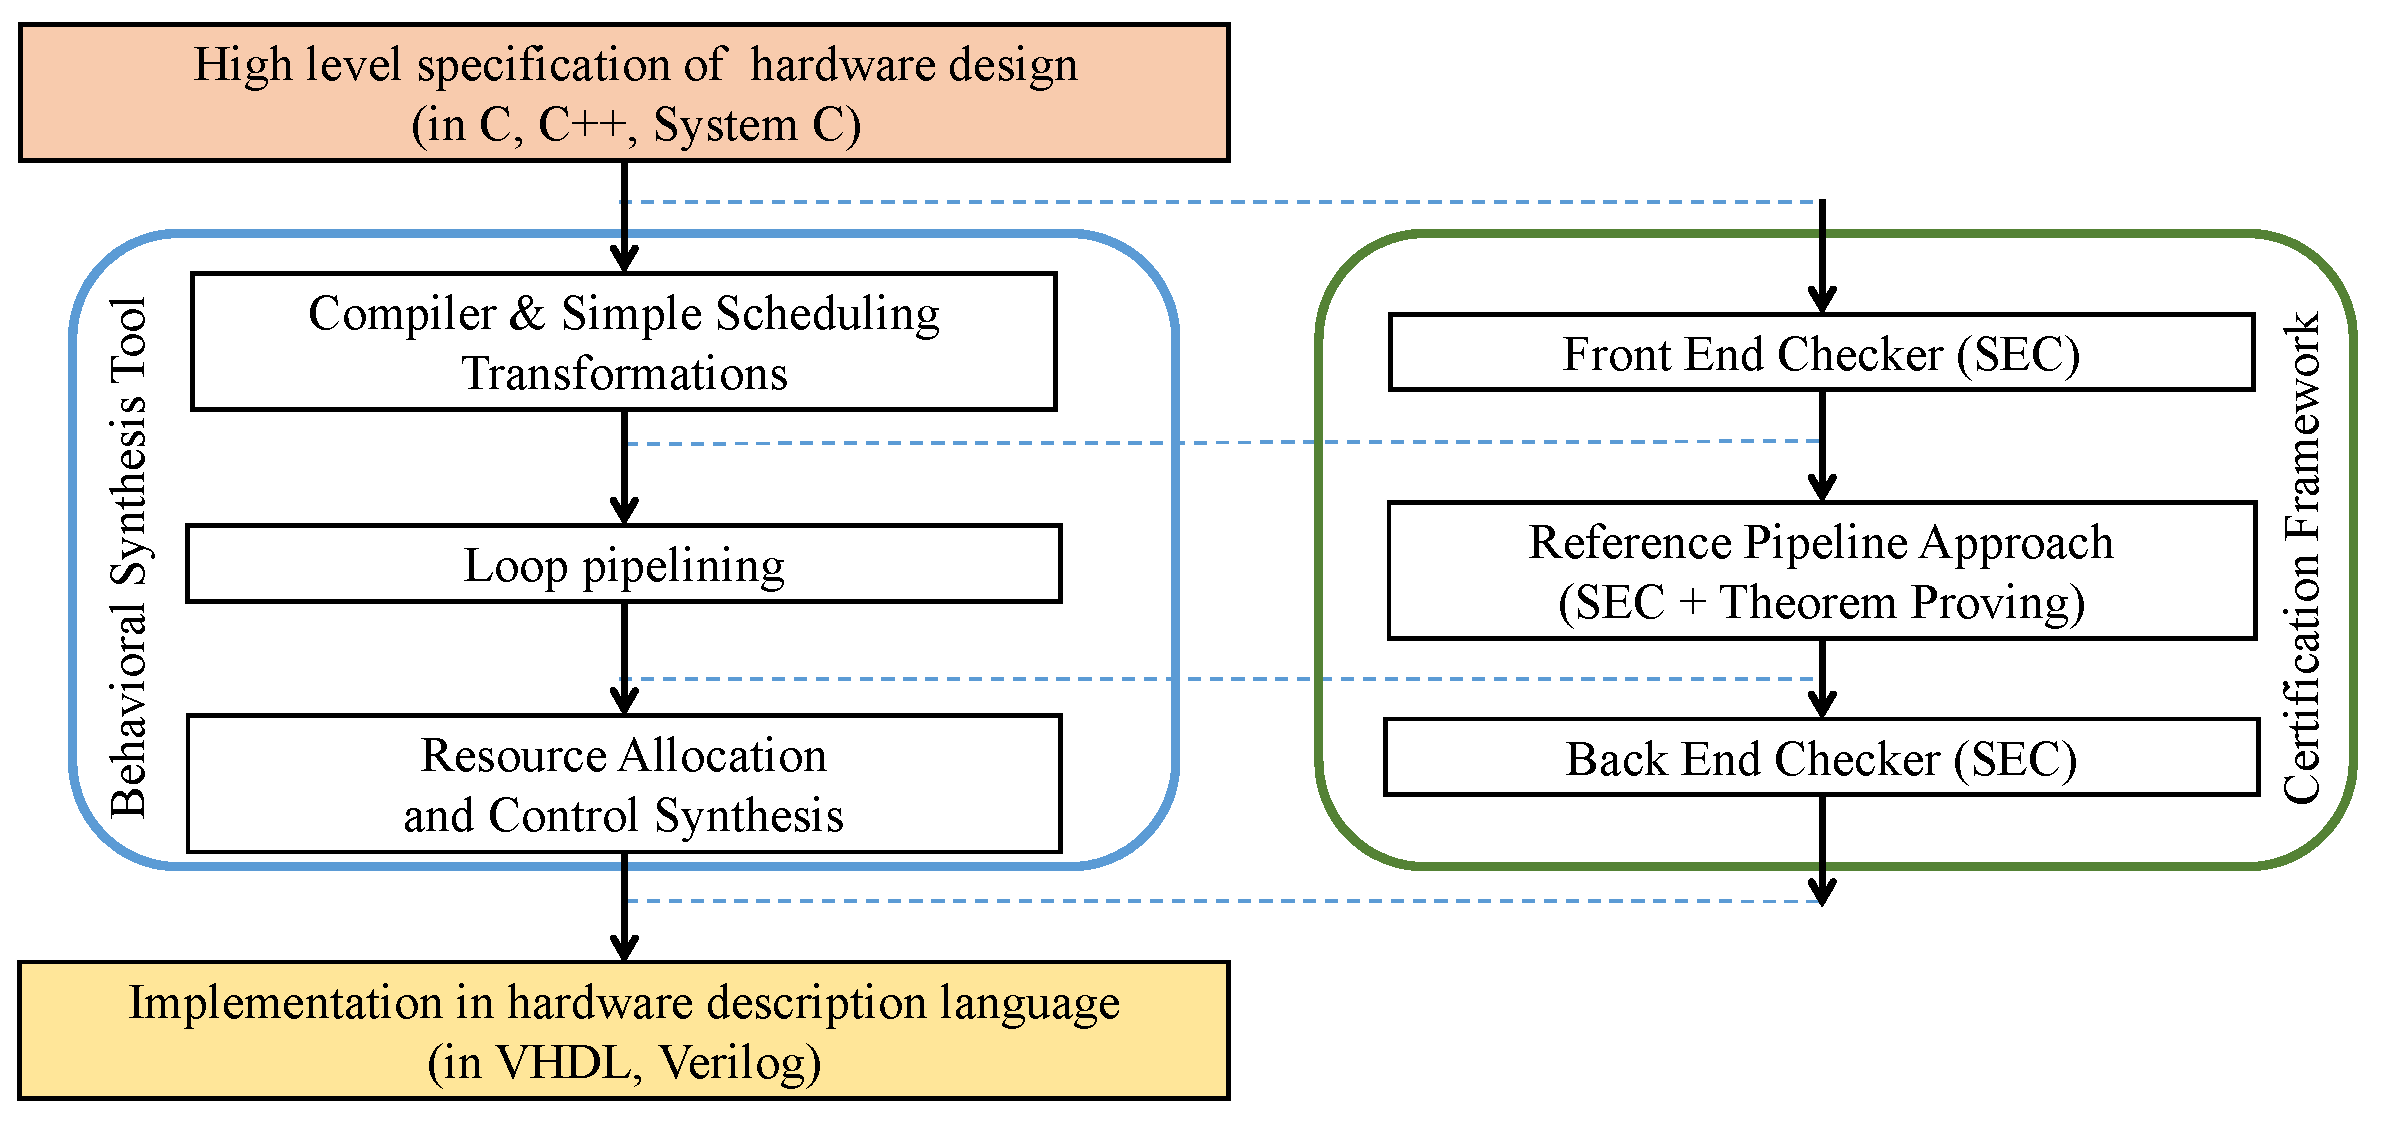
\includegraphics[height=2.8in]{fig-proposal/certification-framework}
\end{tabular}
\end{center}
\caption{Certification model for behaviorally synthesized pipelines}
\label{fig:certification-framework}
\end{figure}

The overall goal of the project is to provide a mechanized framework
for certifying hardware designs synthesized from ESL specifications by
commercial behavioral synthesis tools.
One obvious approach is to apply standard verification techniques (%\eg, 
SEC or
theorem proving) on the synthesized RTL itself.
Unfortunately, such a methodology is not practical.
As mentioned earlier, the large gap in abstraction
between the ESL and RTL descriptions means that there is little
correspondence in internal variables between the two.  Consequently,
direct SEC between the two reduces to cost-prohibitive computation of
input-output equivalence. On the other side, applying theorem proving
is also troublesome since extensive manual effort is necessary and
this effort needs to be replicated for each different synthesized
design. It is also infeasible to
directly certify the implementation of the {\em synthesis tool} via
theorem proving.  In addition to being highly complex and thus
potentially requiring prohibitive effort to formally verify with any
theorem prover, the implementations are typically closed-source and
closely guarded by EDA vendors and thus out of reach of external
automated reasoning communities.

To address this problem, previous work developed two key SEC
solutions, which we will refer to below as {\em Back-end} and {\em
Front-end}.  We then discuss the gap between them, which is being
filled by theorem proving efforts in this dissertation. The certfication model 
is illustrated in Figure~\ref{fig:certification-framework}.
\medskip

\noindent {\bf Back-end SEC:} The key insight behind
back-end SEC is that automated SEC techniques, while
ineffective for directly comparing synthesized RTL with the
top-level ESL description, are actually suitable to compare
the RTL with the intermediate representation (IR) generated
by the tools after the high-level (compiler and scheduling)
transformations have been applied.  In particular,
operation-to-resource mappings generated by the synthesis
tool provide the requisite correspondence between internal
variables of the IR and RTL.  Furthermore, a key insight is
that while the implementations of transformations are
unavailable for commercial EDA tools, most tools provide
these IRs after each transformation application together
with some other auxiliary information.  To exploit these, an
SEC algorithm was developed between the IR (extracted from
synthesis tool flow after these transformations) and
RTL~\cite{rhcxy:atva-09,hxry:date-10,kechengthesis,Yang2013}. 
The approach scales
to tens of thousands of lines of synthesized RTL.

\medskip

\noindent {\bf Front-end SEC:} Of course the back-end SEC
above is only meaningful if we can certify that the input
ESL indeed corresponds to the extracted IR produced after
the compiler and scheduling transformations applied in the
first two phases of synthesis. To address this, another SEC
technique was developed to compare two IRs~\cite{zhenkun:iccd-13,zhenkun2,zhenkun3}.  The idea then
is to obtain the sequence of intermediate representations
$\mbox{IR}_0,\ldots,\mbox{IR}_n$ generated by the compiler
and scheduling transformations, and compare each pair of
consecutive IRs with this new algorithm.  Then back-end SEC
can be used to compare $\mbox{IR}_n$ with the synthesized
RTL, completing the flow.

\bigskip

\noindent {\bf A Methodology Gap:} Unfortunately, the front-end SEC
algorithm can only compare two IRs that are structurally close.  If a
transformation significantly transforms the structure of an IR then
the heuristics for detecting corresponding variables between the two
IRs will not succeed, causing equivalence checking to fail.
Loop pipelining falls in the category of
transformations that significantly change the structure of the IR.
It is a quintessential transformation that changes the control/data
flow and introduces additional control structures (%\eg, 
to eliminate
hazards).  This makes front-end SEC infeasible for its certification.
%On the other hand, it is also a complex and error-prone
%transformation, and ubiquitous across different behavioral synthesis
%tools. 
Furthermore, most commercial implementations are of course
proprietary and consequently not available to us for review; applying
theorem proving on those implementations is not viable from a
methodology perspective.  Thus a specialized approach is warranted for
handling its certification.

\section{A Reference Pipeline Approach}
\label{subsec:reference-pipeline}

\begin{figure}[t!]
\begin{center}
\begin{tabular}{c}
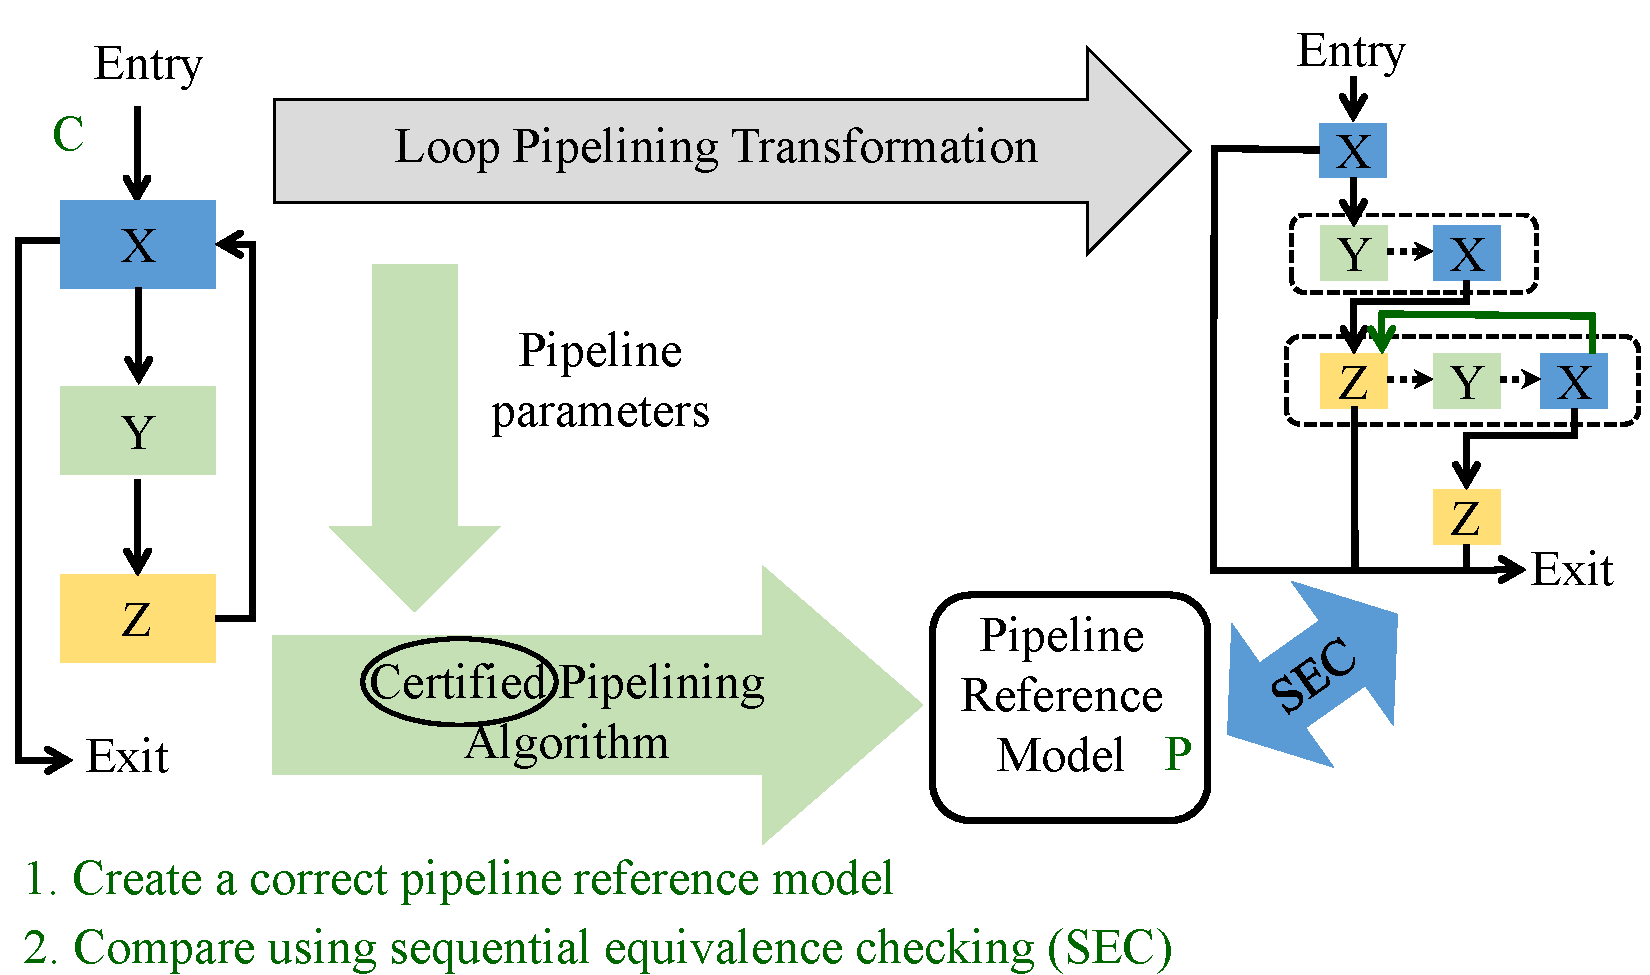
\includegraphics[height=3in]{fig-proposal/ref-pipeline-approach}
\end{tabular}
\end{center}
\caption{Certifying loop pipelining algorithm using SEC and theorem proving}
\label{fig:ref-pipeline-approach}
\end{figure}

To develop a specialized approach for pipelines, a key observation
is that while the transformation {\em implementation} is inaccessible
to us, commercial synthesis tools typically generates a report
specifying pipeline parameters (%\eg, 
pipeline interval, number of loop
iterations pipelined, etc.).  The approach (c.f. Figure~\ref{fig:ref-pipeline-approach})
then is to develop an
algorithm that takes as inputs these parameters and an IR ${\cal{C}}$
for the design before pipelining, and generates a {\em reference
  pipelined IR} ${\cal{P}}$.  Note that this algorithm would be much simpler
than that employed during synthesis; while the former includes
advanced heuristics to {\em compute} pipeline parameters (like
pipeline interval, number of iterations pipelined etc.), this algorithm would merely use
the values provided by its report.  To certify a synthesized RTL with
pipelines, it is sufficient to (1)~check that the {\em given algorithm} can
generate a pipeline ${\cal{P}}$ for the parameters reported by
synthesis, (2)~use SEC to compare ${\cal{P}}$ with the synthesized
RTL, and (3)~prove (using theorem proving) the correctness of this
algorithm.

A previous work~\cite{hrx:dac-12} justified the viability of
steps 1 and 2 above; such a reference pipeline generation algorithm
was developed and used to successfully compare a variety of pipelined
designs across various application domains.  This suggested that the
approach of using a reference implementation is viable for certifying
industrial strength behaviorally synthesized pipelines.  However, a key (and perhaps the
most complicated) component of the approach was missing.  The
algorithm was not verified (indeed, not implemented in a formal
language), rendering the ``certification'' flow unsound.

The unsoundness mentioned above is not just an academic notion.  
The approach showed no systematic approach for
creating the reference pipeline generation algorithm.  In
fact, the specific reference algorithm developed was in fact
heavily influenced by the synthesis tool under consideration
(AutoESL), and highly complex. In
fact, merely by going through the formalization process and thinking
about necessary invariants, we have already found a bug in
the implementation of the algorithm.  
Thus it is critical to develop a mechanized proof of
correctness for this implementation.  Unfortunately, it is not easy to
verify the original pipeline generation algorithm as written.  Its
author was an expert in behavioral synthesis but not in program
verification or theorem proving; consequently, the algorithm, while
simpler than the one implemented in a synthesis tool, was still a highly
complex piece of code.  In particular, since it was not written with
correctness certification in mind, it is difficult to decompose the algorithm into
manageable pieces with succint invariants.

One way to address this problem is to ``buckle down'' and
verify the pipeline generation algorithm (and fixing the
bugs found in the process).  However, a key insight in our
case is that we can get away without verifying such a
complex implementation.  After all, there is nothing
``sacred'' about this specific algorithm for pipeline
generation: given the steps described above, {\em any}
verifiable pipeline generation algorithm would
suffice.\footnote{Note that our algorithm {\em must} create
  a pipeline in accordance with the pipeline parameters
  obtained from the behavioral synthesis tools; otherwise we may
  fail to certify correct designs. However, in practice, we
  have not found this to be a problem.}  Thus the approach
of our dissertation can be viewed as a rational deconstruction of
the pipeline synthesis algorithm of the previous work.  We
identify the key invariant that we need to maintain for
proving computational equivalence between the pipelined and
un-pipelined loops and design an algorithm to explicitly
maintain that invariant.

We discuss the previously proposed algorithm in Chapter~\ref{sec:challenges}
such that we can draw a comparison and better understand the differences
in our implementation of loop pipelining algorithm due to our need to formally certify it.


%We start with a brief summary of behavioral synthesis, highlighting
%the aspects necessary to understand our dissertation thesis.
%the rest of our presentation.
%Note that behavioral synthesis is a complex technology whose
%description is far beyond the scope of this paper.  However, there are
%several behavioral synthesis tools available, including both
%commercial and academic ones, with extensive manuals, documentations
%and tutorials providing user-level description of their
%workings~\cite{spark,xpilot,legup}, and we encourage the
%interested reader to review these materials for further information.

%At a high level, a behavioral synthesis tool can be best viewed as a
%``compiler'' that takes an ESL description and generates RTL.

    \ifoddchapterpage
    \newpage
    \thispagestyle{empty} \mbox{}
    \fi

    %%-------------------------------------------------------------------------
    \chapter{Formalization}
\label{sec:formalization}

\section{Intermediate Representation: CCDFG}

In order to formalize and prove the correspondence between pipelined
and unpipelined IRs, a first step is to define a formalization of the
IRs themselves.  We call our formalization of IRs {\em Clocked Control
  Data Flow Graph} (CCDFG).  An informal description of CCDFG has been
provided before~\cite{rhcxy:atva-09}.  It can be best viewed as a
traditional control/data flow graph used by most compilers, augmented
with a schedule. Control flow is broken into basic blocks.
Instructions are grouped into microsteps which can be executed
concurrently.  A scheduling step is a group of microsteps which can be
executed in a single clock cycle. The state of a CCDFG at a particular
microstep is a list of all the variables of a CCDFG with their
corresponding values.

The semantics of CCDFG require a formalization of the
underlying language used to represent the individual
instructions in each scheduling step.  The underlying
language we use is the LLVM~\cite{llvm}.  It is a popular
compiler infrastructure for many behavioral synthesis tools
and includes an assembly language front-end.  At the point
of this writing we support a limited subset of LLVM, which
however is sufficient to handle all the designs we have
seen.  Instructions supported include assignment, load,
store, bounded arithmetic, bit vectors, arrays, and pointer
manipulation instructions.  We define the syntax of each
type of statement by defining an ACL2 predicate.  For
example, in our syntax, an assignment statement can be
expressed as a list of a variable and an
expression.

An expression can further be of multiple types, %\eg, 
load
expression (loading the value of a variable from memory), add
expression (addition of two variables), xor expression (xor of two variables)
etc., where each expression includes the operation applied to the
appropriate number of arguments.

We provide semantics to these instructions through a
state-based operational formalization as is common with
ACL2.  We define the notion of a CCDFG state, which includes
the states of the variables, memory, pointers, etc.  Then we
define the semantics of each instruction by specifying how
it changes the state.  Thus, for an assignment statement we
will have a function {\tt execute-assignment} that specifies
the effect of executing the assignment statement on a CCDFG
state.

Defining the semantics of most supported statements is
straightforward, with one exception.  The exception is the
so-called ``$\phi$-construct'' available in LLVM.  A
$\phi$-construct is a list of $\phi$-statements.  A
$\phi$-statement is $v := \phi [\sigma, bb1] [\tau, bb2]$,
where $v$ is a variable, $\sigma$ and $\tau$ are
expressions, and $bb1$ and $bb2$ are basic blocks: if it is
reached from $bb1$ then it is the same as the assignment
statement $v := \sigma$; if reached from $bb2$, it is the
same as $v := \tau$; the meaning is undefined otherwise. The
construct is complex since the effect of executing this
statement on a CCDFG state $s$ depends not only on the state
$s$ but also on how $s$ is reached by the control flow.
Unfortunately, $\phi$-statements are required in loop designs ---
they are used to evaluate the value of loop carried dependencies.
Consequently, the complexity induced
by this instruction cannot be avoided.

\section{Correctness of Loop Pipelining}
%A behavioral synthesis tool automatically generates a RTL design from an ESL design through a series of
%transformations. Pipelining a loop is a critical
%transformation in behavioral synthesis.

For the purposes of this paper, a {\em pipelinable loop} is
a loop with the following restrictions~\cite{hrx:dac-12}:
\begin{enumerate}
\item no nested loop;
\item only one $Entry$ and one $Exit$ block; and
\item no branching between the scheduling steps.
\end{enumerate}

{\bf Discuss with Sandip Sir}: We should mention that there is only one conditional branch and one unconditional branch related to loop,
others can be handle via previous compiler transformations. Also, there is only one phi statement. 

These restrictions are not meant to simplify the problem, but reflect
the kind of loops that can be actually pipelined during behavioral
synthesis.  For instance, synthesis tools typically require inner
loops to have been fully unrolled (perhaps by a previous compiler
transformation) in order to pipeline the outer loop.

\begin{figure}
\begin{center}
\begin{tabular}{ccc}
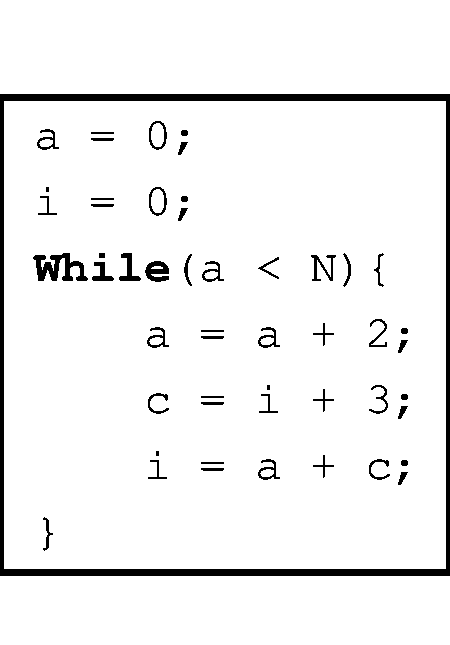
\includegraphics[height=1.6in]{fig-proposal/C-code}
&
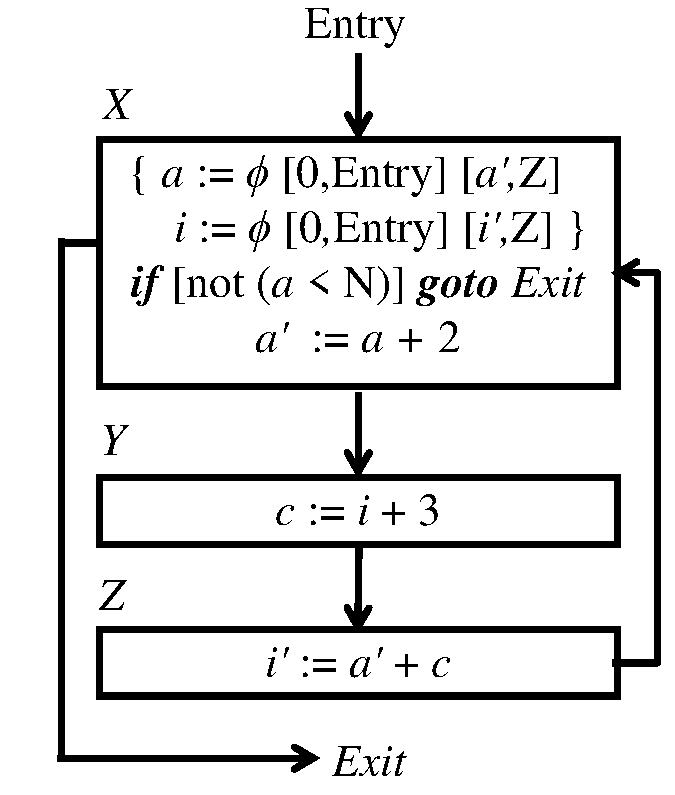
\includegraphics[height=1.6in]{fig-proposal/seq-ccdfg-1}
&
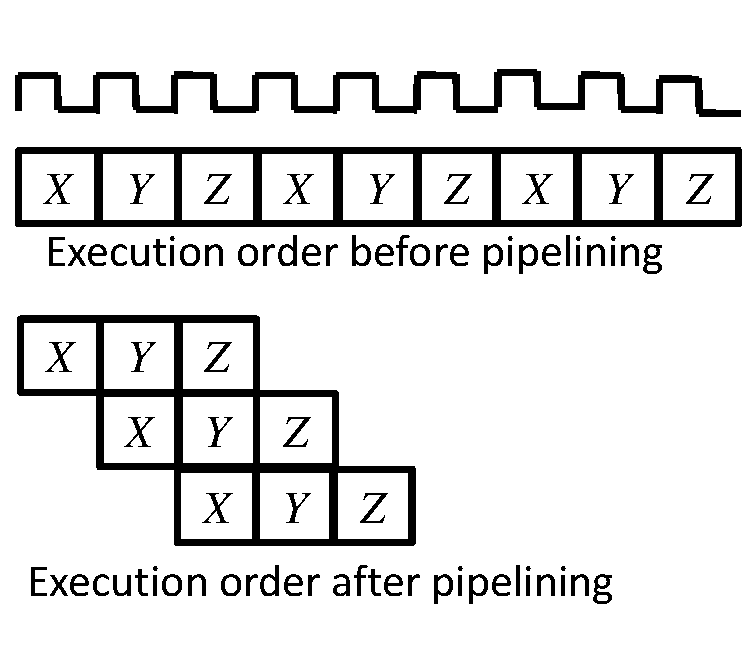
\includegraphics[height=1.6in]{fig-proposal/pp-clock-cycles}
\\
(a) & (b) & (c)
\end{tabular}
\end{center}
\caption{(a) Loop in C; (b) Loop CCDFG before pipelining ({\bf Note for Disha: create a better figure. Discuss with Zhenkun}) ; (c) Pipelining increases throughput}
\label{fig:high-level-synthesis}
\end{figure}

Figure~\ref{fig:high-level-synthesis}(a) illustrates the C
code (ESL description) for a loop.  The C code does not have
a schedule or the concept of a clock cycle.
Figure~\ref{fig:high-level-synthesis}(b) shows CCDFG of the
sequential loop just before loop pipelining. The loop has
three scheduling steps: $X$, $Y$ and $Z$.  The scheduling
step before the loop is $Entry$ and after the loop is
$Exit$. Note that there is a $\phi$-statement in the
first scheduling step of the loop.  This $\phi$-statement
accounts for those variables whose values are dependent on
the variables evaluated in a previous iteration.

Behavioral synthesis tools use complicated heuristics and aggressive scheduling strategies to
find an optimized pipeline interval (clock cycles after which a new iteration can be started such that there are no data hazards). One iteration of the sequential design takes three
clock cycles. Observe in Figure~\ref{fig:high-level-synthesis}(c) that with the pipeline interval of one, the three iterations of the pipelined loop
take five clock cycles as opposed to nine clock cycles in the sequential loop.
Loop pipelining reduces the number of clock cycles required to execute the loop, hence this transformation is used by synthesis tools to increase throughput and reduce overall latency.

%% Since, reasoning about execution becomes difficult if we have to
%% always keep track of the previous scheduling step, we treat the first
%% iteration of the sequential CCDFG {\em seq-pre-loop} as a separate
%% iteration than the rest of the iterations {\em seq-loop}.  Infact, the
%% first step of our pipelining algorithm is to unroll the loop once and
%% replace $\phi$-construct by corresponding assignment statements based
%% on the previous scheduling steps.

%% \subsection{Correctness Statement}
%% \label{subsec:correctness-defn}

%% IMPORTANT : take a look again, if we want to keep all iterations same, we can start from k = 0

 \smallskip
\noindent {\textbf {Correctness Statement:}}
Let $L$ be a loop in CCDFG $C$, and let $L_{\alpha}$ be the
pipelined implementation generated by a pipeline algorithm using
pipeline parameters $\alpha$.  Let $V$ be the set of
variables in $L$, and $U$ be the set of all
variables in $C$.  Suppose we execute $L$ and $L_{\alpha}$
from CCDFG states $s$ and $s'$ respectively, such that for
each variable $v\in V$, the value of $v$ in $s$ is the same
as that in $s'$, and suppose that the state on termination
are $f$ and $f'$ respectively.  Then (1)~for any $v\in V$,
the value of $v$ in $f$ is the same as that in $f'$, and
(2)~for any $v\in(U\backslash V)$, the value of $v$ in $f'$
is the same as that in $s'$.

\medskip
\noindent
{\em Remark:} Condition (2)
ensures that variables in $C$ that are not part of the loop
are not affected by $L_{\alpha}$.  The value of any new
variables introduced by the algorithm in $f'$ are irrelevant since they are not accessed
subsequently.


%% Important: Ask Sandip: How are we accounting for condition 2 in our correctness statement ??? Am I missing something??

%\begin{quote}
%Let $L$ be a loop in CCDFG $C$, and let $L_{\alpha}$ be the
%pipelined loop CCDFG. Let $V$ be the set of
%variables mentioned in $L$, and $U$ be the set of all
%variables in $C$.  Suppose we execute $L$ and $L_{\alpha}$
%from CCDFG states $s$ and $s'$ respectively, such that for
%each variable $v\in V$, the value of $v$ in $s$ is the same
%as that in $s'$, and suppose that the state on termination
%are $f$ and $f'$ respectively.  Then (1)~for any $v\in V$,
%the value of $v$ in $f$ is the same as that in $f'$, and
%(2)~for any $v\in(U\backslash V)$, the value of $v$ in $f'$
%is the same as that in $s'$.
%\end{quote}
%\noindent
%{\em Remark:} Condition (2) is the {\em frame rule} which
%ensures that variables in $C$ that are not part of the loop
%are not affected by $L_{\alpha}$. The algorithm introduces
%additional variables, eg, {\em shadow variables}
%(cf. Section~\ref{sec:proof}).  The values of these
%variables in $f'$ are irrelevant since they are not accessed
%subsequently.



%\medskip
%\noindent{{\bf CCDFG :}} Formalizing the correctness
%statement entails defining the semantics of CCDFG.  A CCDFG
%is a control/data flow graph augmented
%with a schedule.
%Control flow is broken into basic blocks.  Instructions in a
%basic block are grouped into {\em microsteps} that are
%executed concurrently.  A schedule is a grouping of
%microsteps which can be completed within one clock cycle.
%The instruction language we support is a subset of
%LLVM~\cite{llvm} which is a front-end for many behavioral
%synthesis tools~\cite{autoesl,xpilot,legup}; we support
%assignment, load, store, bounded arithmetic, bit vectors,
%arrays, and pointer manipulations.  As is common with ACL2,
%we use a state-based operational semantics.  Assigning
%meanings to most instructions is standard; one exception is
%the $\phi$-statement ``{\tt v := phi [$\sigma$ bb1] [$\tau$
 %   bb2]}''.  If reached from basic block {\tt bb1}, it is
%the same as the assignment statement {\tt v := $\sigma$}; if
%reached from {\tt bb2}, it is the same as {\tt v := $\tau$};
%the meaning is undefined otherwise.  Reasoning about
%$\phi$-statement is complex since after its execution from
%state $s$, the state reached depends not only on $s$ but
%previous basic block in the history. However,
%We need to
%handle it since it is used extensively to implement loop
%tests.  Indeed,
%A key step in loop pipelining is
%$\phi$-elimination, \viz, unrolling the loop once and
%replacing the $\phi$-statement with assignment statements
%(cf. Fig.~\ref{fig:loop}).









    \ifoddchapterpage
    \newoddpage
    \fi


    %-------------------------------------------------------------------------
    \chapter{Research Challenges}
\label{sec:challenges}

\section{Previously Proposed Algorithm}
\label{subsec:kecheng's algorithm}

\noindent
Given a set of microsteps $M$, a set of edges $E$, and a schedule $S$ of a
sequential CCDFG, and pipeline parameters (pipeline
interval $I$ and number of scheduling steps in the loop
$N$), the algorithm~\cite{hrx:dac-12} generates new microsteps, edges and
schedule for the pipelined CCDFG. Values of these inputs are readily available from
intermediate feedback reports from the behavioral synthesis
tool. Given CCDFG $C$, this algorithm replaces
each loop $L$ in $C$ with the pipelined refinement of
$L$. The steps of the algorithm are explained below with the
help of the example introduced earlier in Figure~\ref{fig:high-level-synthesis}(a).

\begin{figure}
\begin{center}
\begin{tabular}{cc}
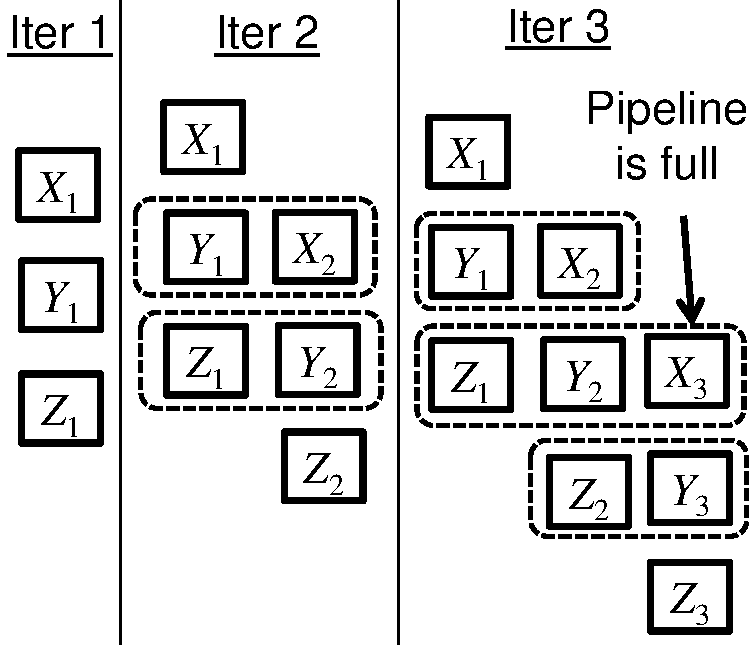
\includegraphics[height=1.7in]{fig-proposal/generate-scheduling-steps}
& %\hspace{0.1cm}
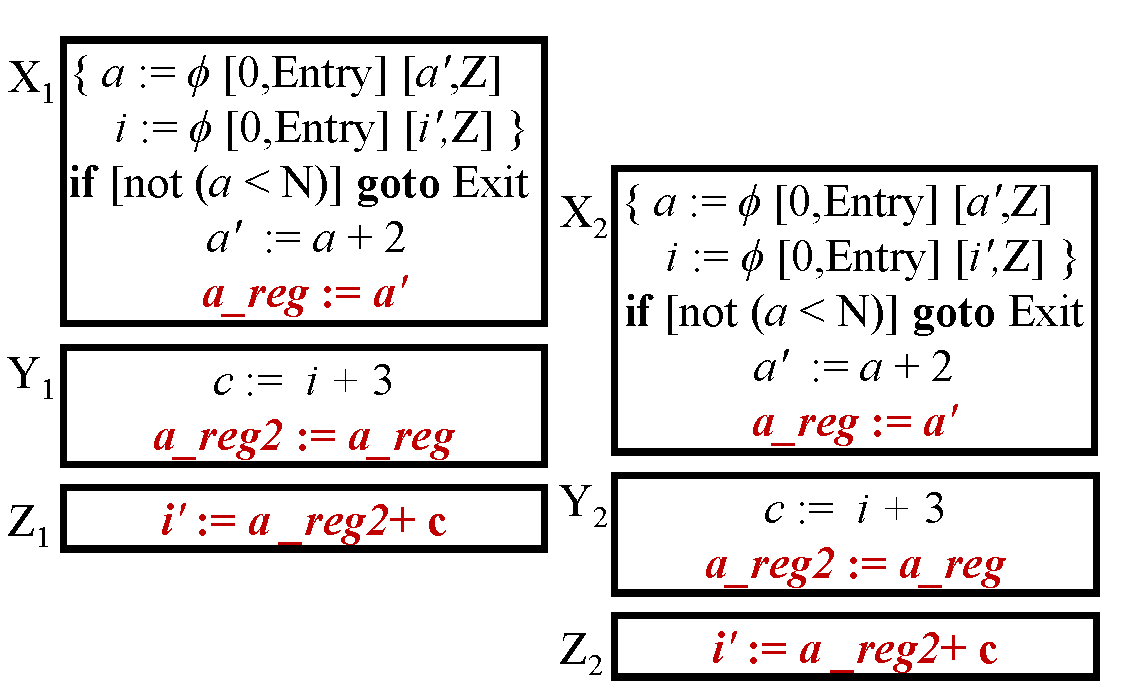
\includegraphics[height=1.7in]{fig-proposal/shadow-reg}
\\
(a) & (b)
\end{tabular}
\end{center}
\caption{(a) Generate scheduling steps. After the pipeline is full, adding new iteration simply repeats the pipeline full stage. (b) Generate shadow registers.}
\label{fig:algorithm}
\end{figure}

%\begin{enumerate}[--]
{\bf Generate scheduling steps:} Figure~\ref{fig:algorithm}(a) shows the addition of scheduling steps of new iterations of a loop according to the pipeline interval. Here, the loop has three scheduling steps and a pipeline interval of one. The new scheduling steps are generated till the pipeline is full. This step generates a new schedule.
For the sake of easily identifying microsteps later, every microstep in the unrolled loop is given a unique name even though
a microstep is the same across different iterations. We would later see how
this trivial step affects the theorem proving process adversely.

{\bf Generate shadow registers:} In order to pipeline a loop, we have to remove data hazards. We first identify all variables that can be overwritten when executing overlapped iterations and then introduce new temporary variables called shadow registers to avoid overwrites. In Figure~\ref{fig:algorithm}(b), the value of $a'$ will be overwritten in $X_2$ before $Z_1$ can read it. So, we introduce a new pipeline register $a\_reg$ which gets assigned the value of $a'$ and replace subsequent reads of $a'$ with reads of $a\_reg$. In the next scheduling step, $a\_reg2$ is assigned the value of $a\_reg$ and further subsequent reads of $a'$ are replaced with reads of $a\_reg2$. Introducing shadow registers in such a way removes the possibility of data hazard as the value of the old variable is stored in a new temporary shadow variable every scheduling step.

\begin{figure}[t!]
\begin{center}
\begin{tabular}{cc}
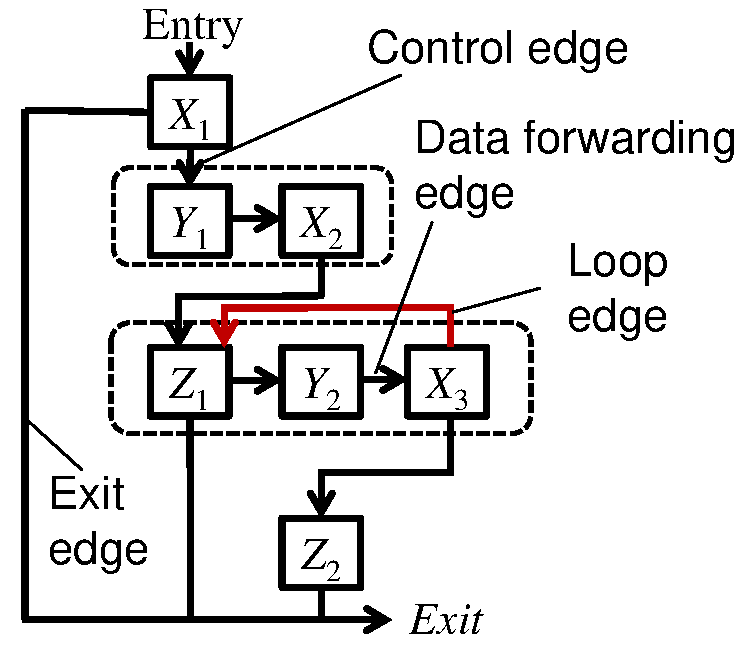
\includegraphics[height=1.6in]{fig-proposal/generate-edges}
& %\hspace{0.1cm}
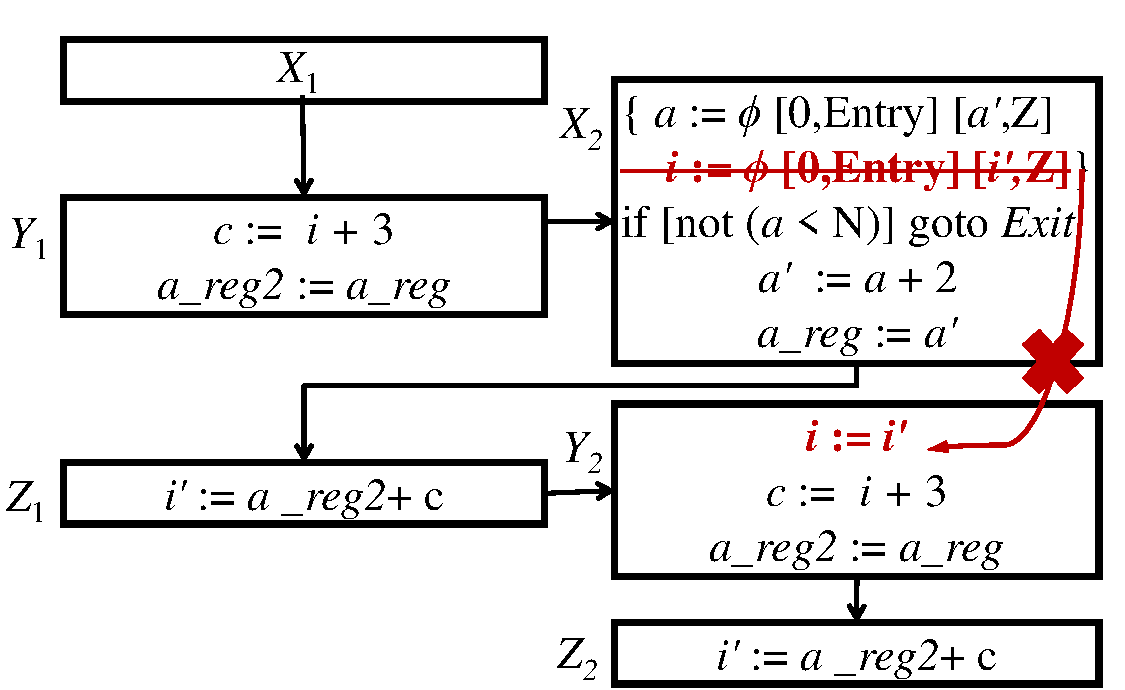
\includegraphics[height=1.6in]{fig-proposal/data-forwarding}
\\
(a) & (b)
\end{tabular}
\end{center}
\caption{(a) Generate edges for pipelined CCDFG (b) Data propagation.}
\label{fig:algorithm-2}
\end{figure}

{\bf Generate edges:} The algorithm adds the edges for data and control flow as shown in Figure~\ref{fig:algorithm-2}(a). Control edges are edges from one scheduling superstep to the next. Data forwarding edges forward data from one scheduling step to the next in a single scheduling superstep. Loop edge denotes the repetition of the pipeline full stage. Exit edges are from the scheduling steps to the $Exit$ block. Note that a pipelinable loop has only one $Exit$ block. Even though the concept of $Exit$ edges was introduced, but they were not implemented in the algorithm.

{\bf Generate data propagation:} In Figure~\ref{fig:algorithm-2}(b), we require the value of $i'$ in $X_2$ to execute the following statement:
$$ i := \phi [0, Entry][i', Z]$$
But, if we execute $X_2$ before executing $Z_1$, the value of $i'$ has not yet been produced. To avoid such a situation, the algorithm relocates the assignment statement $i := i'$ to $Y_2$ just before it needs to be read. The assignment statement $i := i'$ is obtained from the $\phi$-statement $i := \phi [0, Entry][i', Z]$ since in the sequential execution, we would have entered $X_2$ from $Z$ block.

This relocation is however incorrect. Note that we have moved the assignment statement across the conditional branch. $$ if [not (i<N)] goto Exit $$ If we would have executed the sequential CCDFG and the exit condition in the second iteration is true, we would have executed the microstep $i := i'$ before exit. However, now in the pipelined CCDFG, if we exit in $X_2$, we do not execute the microstep $i := i'$. Hence, the value of $i$ is not same in the sequential and pipelined CCDFGs. This is a bug that we found in this algorithm: it incorrectly allows relocation of microsteps across conditional branch statements.
We realized that the authors of the previous proposed algorithm had not accounted for the exit conditions while testing the algorithm. As a result, this bug was not found prior to our formalization. We provide a fix to this bug in our loop pipelining algorithm in Section~\ref{sec:pipelining-algorithm}.

Even after we fix the bug in the proposed algorithm, it is not easy to verify this algorithm as it is.
We elaborate below on the challenges
in verifying the proposed algorithm and in general, any complex algorithm not written while keeping theorem proving in mind.
%\end{enumerate}

\section{Challenges associated with Formal reasoning}

To understand the complexities involved in mechanical
certification of an algorithm that was not designed
originally with certification in mind, we need to re-visit
the general approach to applying formal reasoning on
software programs.  The typical approach is to break the
program into a number of pieces, prove key lemmas
characterizing the role of each piece, and then chain these
lemmas together into a proof of the correctness of the
entire program. Crucial to this approach, however, is the
requirement that each program piece can be characterized by
a succinct invariant that can be easily verified.  However,
in a program not developed with reasoning in mind,
optimizations typically destroy the structural disciplines
and modularity of the individual program pieces. This makes it
difficult to identify and isolate the components that
actually maintain succinct, interesting invariants.

For instance, to prove the correctness statement in the previous algorithm, 
we want to prove that the complete algorithm follows
the invariant that the semantic run of input CCDFG is equal to semantically running the output CCDFG.
Since the algorithm is composed of four concrete steps -- generate scheduling steps, add shadow register,
add edges and data propagation, we intuitively expect the individual steps or at least a combination of steps in sequence to
follow this invariant. However, since the algorithm has not been designed keeping theorem proving
in mind, that is not the case. For example, if
we consider the first step of the proposed algorithm -- {\bf generating new scheduling steps} by
overlapping executions of an unrolled loop, we know that the execution 
of the sequential scheduling steps is not the same as the execution of new scheduling steps
unless we prove that there are no data hazards. But, data hazards are not completely eliminated till the last step of the algorithm. Note, that the complete algorithm does follow the invariant as expected, but reasoning about the structure of the
complete algorithm at once is not easy.

Our first approach was to certify their implementation as it is using theorem proving. 
But, our experience was that it is a difficult approach, one that we need not endure.
In general, in order to certify such an arbitrary implementation,
one has to either (1)~restructure the implementation into
one that is more disciplined, and prove the equivalence
between the two, or (2)~come up with very complex
invariants that essentially comprehend how invariants from
each individual piece are conflated together in the
implementation.  Both approaches require extensive human
interaction, resulting in the proverbial euphemism of proofs
of programs being orders of magnitude more complex than the
programs themselves~\cite{liu}.
%In addition, the previous algorithm does not take a CCDFG as input, but rather
%works with microsteps, edges and schedule of a CCDFG. That can get tricky because to analyze the
%semantic run of a CCDFG, we have to now simultaneously analyze all the three inputs. In our approach,
%we work with the CCDFG itself and define the run of a CCDFG semantically.

%Furthermore, the previous algorithm initially unrolls the loop and later adds
%a back edge to mimick the pipeline full stage. Unrolling loop with unique names
%for each microstep makes it easier to design the algorithm but formally we lose the notion
%that each microstep is part of a loop and not different in each iteration.
%Besides, unrolling loop makes it very difficult to reason for the correctness of the
%back edge in the
%full pipeline stage.

In our work, however, we can ``get away'' without verifying
the specific implementation while still being able to
certify the design generated by behavioral synthesis without
loss of fidelity. The key observation, as above, is that it
is sufficient to develop {\em any} certifiable algorithm
that generates a pipelined CCDFG from a sequential
implementation which can be effectively applied with SEC.
In particular, any certifiable algorithm that has the same
input-output characteristic as the proposed algorithm
is sufficient.  Thus, our dissertation is on identifying
certifiable primitives and invariants of a loop pipelining
transformation and developing a pipeline generation
algorithm using those primitives, achieving the dual goal of
mechanical reasoning of the algorithm and amenability of the
resulting reference model to SEC.

\section{Importace of using Formal Methods for checking correctness}

Formally verifying an algorithm gives confidence that the pipelined design is indeed correct. We can claim that if a pipeline loop is created, then there are no additional data hazards which have not been accounted for. Also, since our final theorem proves that executing a sequential loop is same as executing the pipelined loop generated from our algorithm, we can confidently say that our algorithm is complete and data and control flows are well-maintained.   

Checking correctness using formal methods prompted us to address the issues lacking in the previous algorithm. To ensure that control flow is maintained, we had to deal with branches. The previous algorithm introduces the concept of Exit edges but does not explain/implement them. The previous authors checked the output of their algorithm with RTL under the assumption that the loop never exits, hence they did not face any issue while testing. However, removing a conditional branch in a loop and furthermore, adding the conditional branch back in the middle of a pipelined loop requires complex reasoning which we manage using one of our primitives, explained in ~\ref{sec:pipelining-algo}.

Also, the invariant that data flow is maintained at each step enabled us to find a bug in the previous algorithm. The previous algorithm moves a statement to make sure one particular data hazard is removed, but in doing so they move the statement across a conditional branch statement. Our primitves ensure that such a move is not possible. We have restructred the data propagation step so that instead of going across a conditional branch in the same iteration, the movement of step is now to the previous iteration, explained in ~\ref{sec:pipelining-algo}. 

%Furthermore, there is a different mindset required when we merely write an algorithm Vs when we want to prove an algorithm using theorem proving. For example, adding a shadow register step may look like a trivial step which requires simple reasoning about read and write variables, but when we have to mathematically prove that such a step maintains the control and data flow, we have to reason about the fact that the new variable is indeed a new variable not introduced anywhere else in the algorithm. 



    \ifoddchapterpage
    \newoddpage
    \fi

    %%-------------------------------------------------------------------------
    \chapter{Our Approach}
\label{sec:pipelining-algorithm}

As mentined earlier, one of the most complex requirement of 
verifying behaviorally synthesized pipelined designs is a certified loop
pipelining algorithm which can generate a pipeline reference model
for varied designs. This pipeline reference model must have a similar structure to the pipelined RTL generated by behavioral synthesis tools such that they can be compared using SEC. 
  
Pipeline synthesis is based on the key observation that
execution of successive iterations can be overlapped without affecting 
execution as long
as data and control dependecies are correctly maintained. 
Thus, the three main
activities of a pipeline synthesis algorithm are to
(1)~identify and remove possible hazards (2)~overlap the
successive iterations according to the pipeline interval, and (3)~ensure proper placement of conditional and unconditional branches. In our case,
the identification of data hazards is simplified since the synthesis tool
provides a pipeline interval. If we can use this pipeline interval to build our design, then the pipeline reference model is comparable to RTL in abstraction. Thus, instead of {\em
discovering} a pipeline interval ourselves by analyzing read and write variables of every design so that no
hazard is introduced, we reuse the provided interval. 
We have developed a framework of five certified pipelining
primitives which allows us, among other things, to prevent possible data
hazards. Our framework also provides a primitive
to overlap successive iterations and a provision to add and remove branches when required while still maintaining the control flow. We now discuss
the framework as shown in Figure~\ref{fig:primitives}  in detail.

\section{Framework of Provable Pipelining Primitives}

\begin{figure}[t!]
\begin{center}
\begin{tabular}{c}
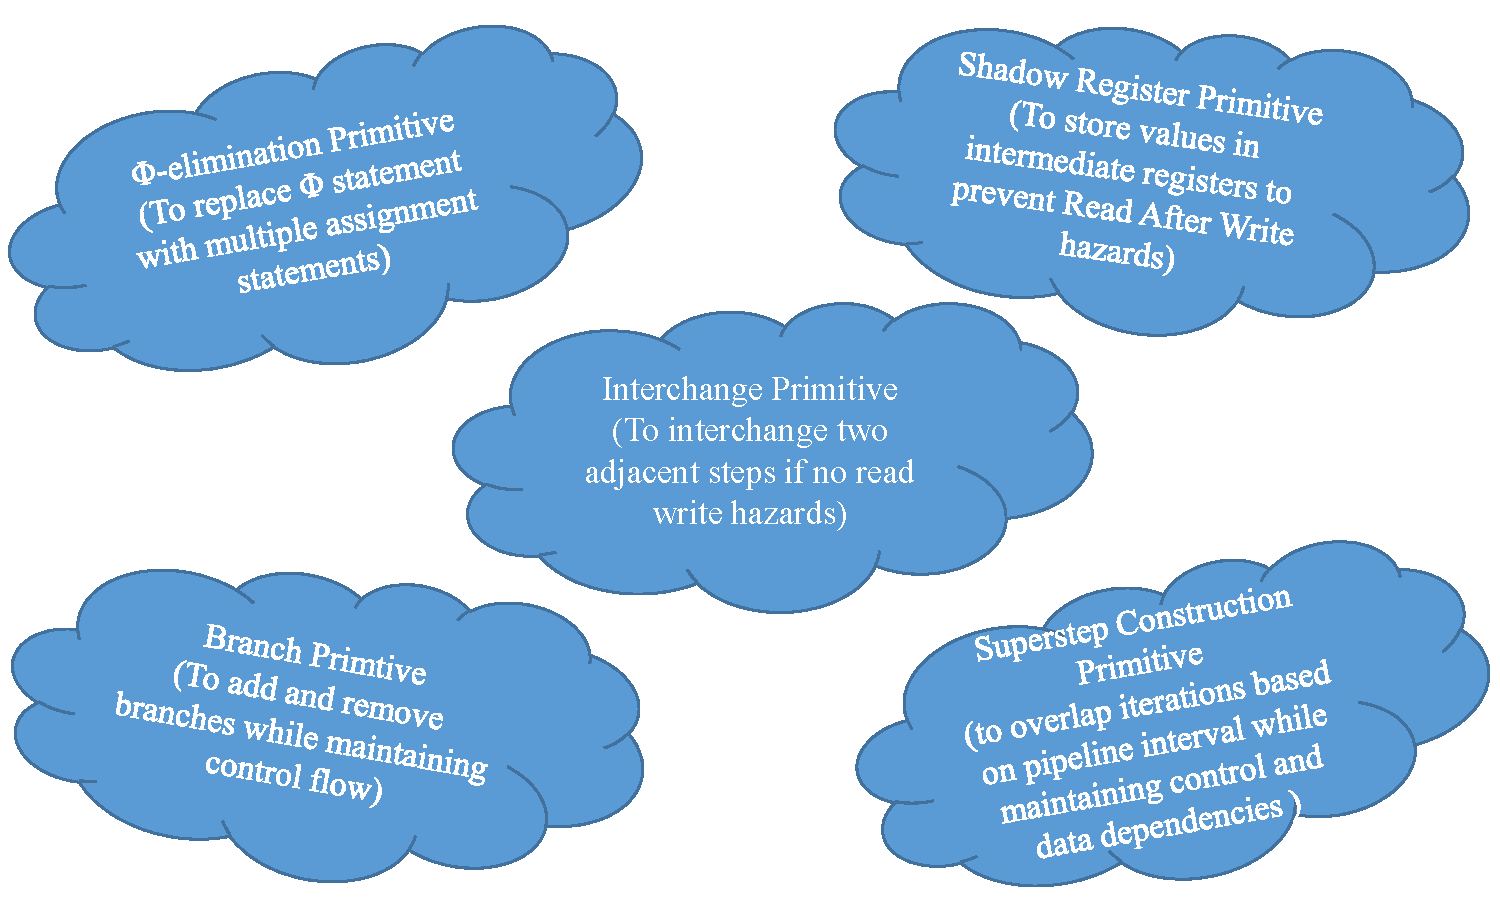
\includegraphics[width=5.5in]{fig-proposal/primitives}
\end{tabular}
\end{center}
\caption{Our framework of certified primitives}
\label{fig:primitives}
\end{figure}

We believe that the following primitives are necessary and essential in creating any pipelining
algorithm in behavioral synthesis.

{\textbf {$\phi$-elimination primitive}} -- A $\phi$-statement is ``{\tt v = phi
[$\sigma$ X] [$\tau$ Y]}'', where {\tt v} is a
variable, $\sigma$ and $\tau$ are expressions, and {\tt X}
and {\tt Y} are basic blocks: while execution, if the $\phi$-statement is
reached from {\tt X} then it
is the same as the assignment statement
{\tt v = $\sigma$}; if reached from {\tt Y}, it is the same as {\tt v = $\tau$};
the meaning is undefined otherwise.
Reasoning about the $\phi$-statement is complex since after its
execution from a state, say $s$, the state reached depends not only
on the state $s$ but also on previous basic blocks in the execution history.
However, we must handle it since it is used extensively in
loops to perform different actions depending on whether the
loop body is executed the first time. One of the key steps in loop pipelining is,
therefore, $\phi$-elimination {\em i.e.}, replacing
$\phi$-statement with appropriate assignment statements when the previous basic block is explicitely known.

\begin{figure}[t!]
\begin{center}
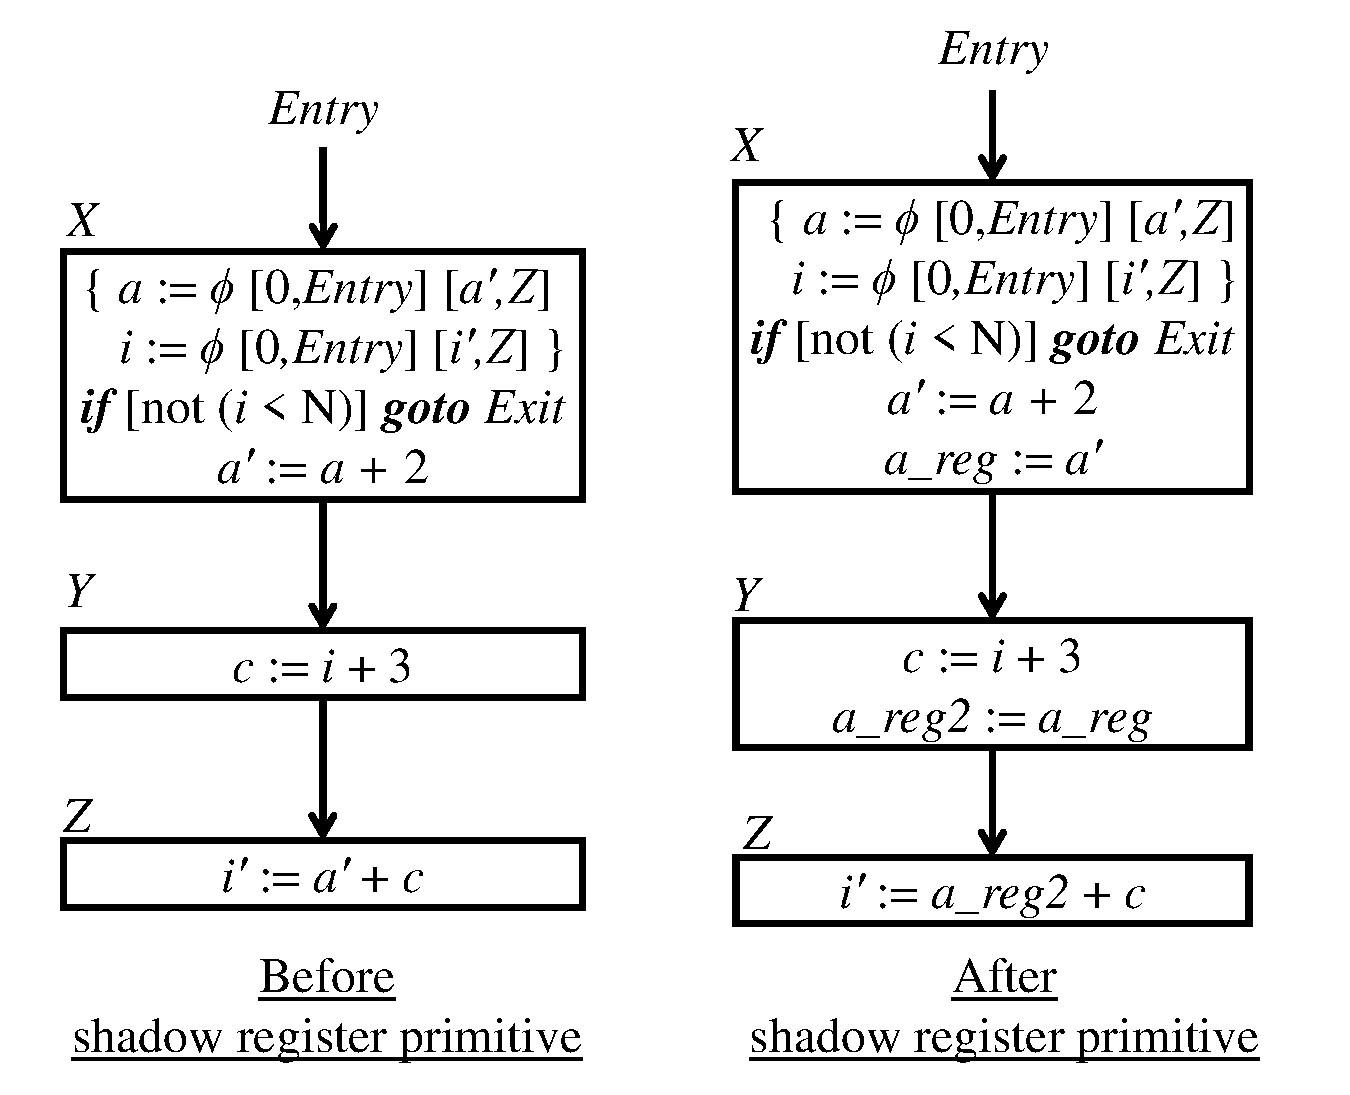
\includegraphics[height=3.3in]{fig-proposal/shadow-reg-primitive}
\end{center}
\caption{Shadow register primitive}
\label{fig:primitives1}
\end{figure}

{\textbf {Shadow register primitive}} -- We define a shadow register microstep as simply an assignment
statement with symbol expression ($x$) assigned to a new value ($x\_reg$). We call all the new introduced variables as shadow registers. Intuitively, it is correct that in a
sequence of steps, if we assign a variable to a shadow register and replace all occurences of $x$ with $x\_reg$
till the next write of $x$, we should
not have made any difference in the execution. Also, since we are not changing the value of $x$ itself,
 the state after end of execution for both CCDFGs as far as real variables are concerned (all variables
 excluding all shadow registers) is same. In Figure~\ref{fig:primitives1}, if we assign a shadow register
 $a\_reg$ value of $a'$ at the end of $X$ block, shadow register $a\_reg2$ value of $a\_reg$ in $Y$ and replace the read occurence of $a'$ in $Z$ with $a\_reg2$, the sequential execution remains same.
But, because of the addition of these shadow registers, the value of $a'$ is stored in a new temporary variable in every new scheduling step which prevents data hazards.

\begin{figure}[H]
\begin{center}
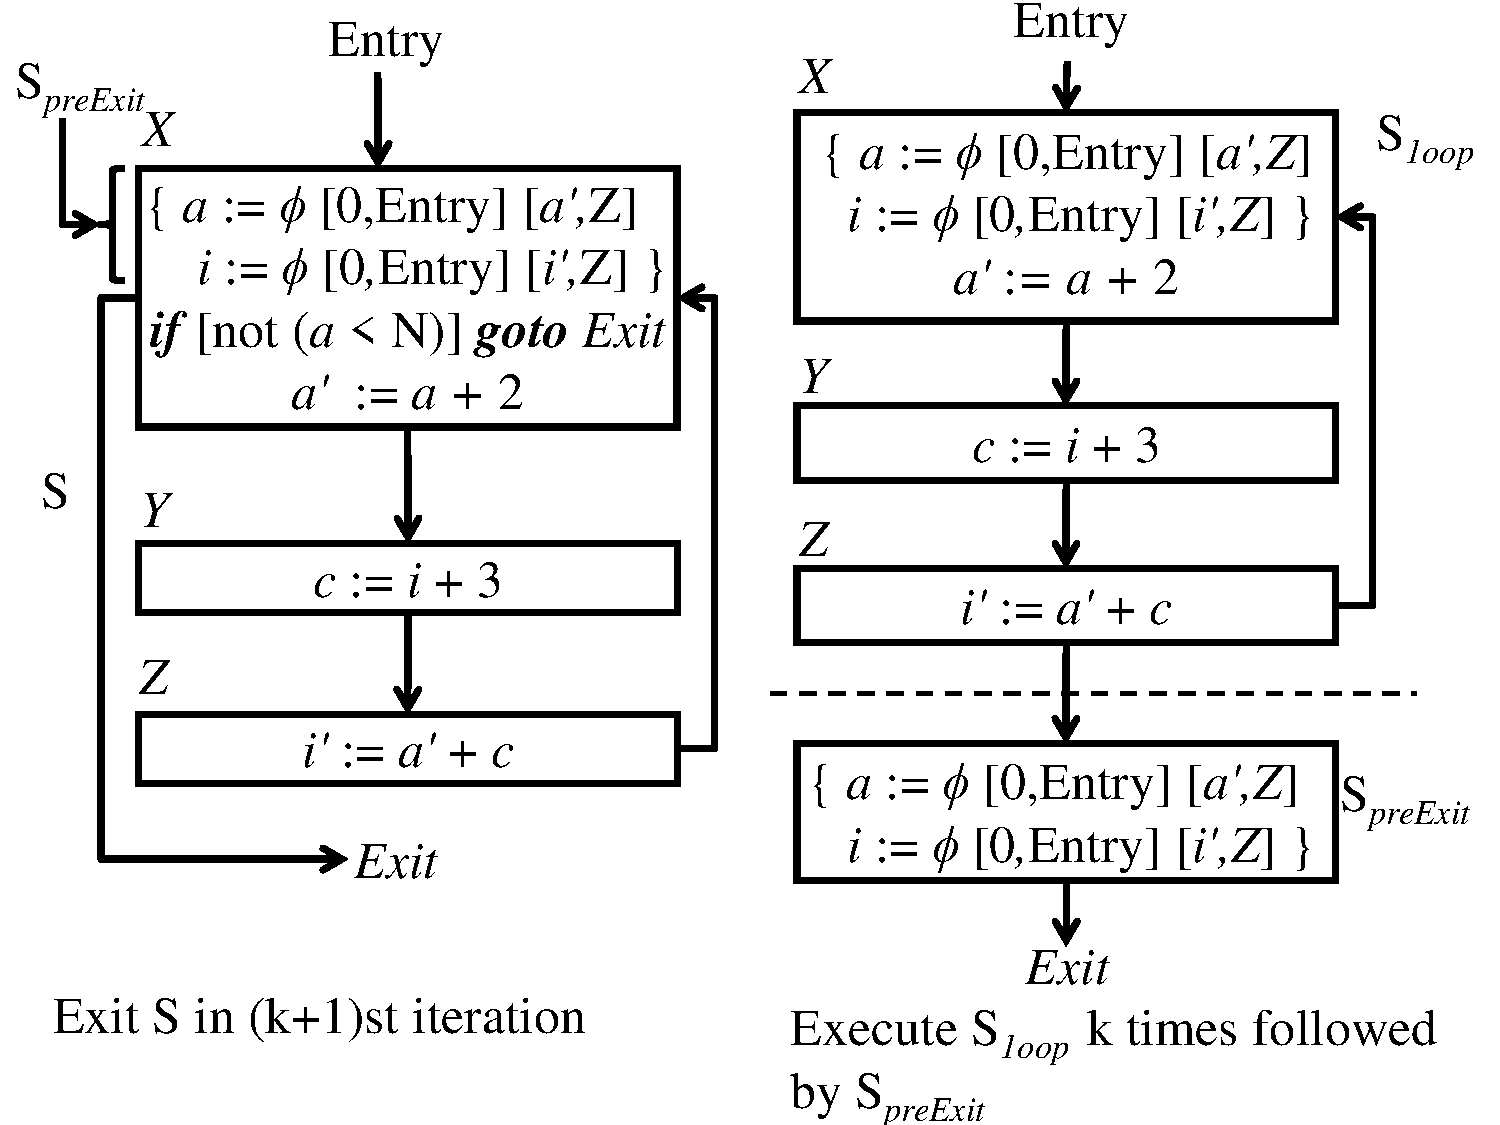
\includegraphics[height=3.3in]{fig-proposal/conditional-branch-primitive}
\end{center}
\caption{Branch primitive}
\label{fig:branch-primitive}
\end{figure}

{\textbf {Branch primitive}} -- Branch instructions are required to determine the control flow. However, reasoning about execution of branch instructions in a loop everytime we apply a primitive can make proof very complex.
We note that if we specifically assume that the exit condition becomes true after completing $k$ iterations, then we can remove the conditional branch.
To understand the branch primitive (c.f. Figure~\ref{fig:branch-primitive}), 
let's assume there is a conditional branch in the sequential loop structure $S$, which points to either
the next microstep in sequence or exits the loop by branching to the scheduling step
$Exit$. Let $S_{preExit}$ be the collection of microsteps before this branch in $S$ and
let $S_{loop}$ be the corresponding CCDFG loop without the conditional branch.
The conditional branch primitive allows us to replace $S$ with $S_{loop}$ followed by
$S_{preExit}$. Similarly,
the primitive also allows us to introduce an exit conditional branch by replacing
$S_{loop}$ followed by $S_{preExit}$ with $S$.
Note that since $k$ can take any value $k \ge 0$, we are not compromising on the correctness statement.  
It can be proved that executing $S$ $k$ times such that it exits in the $(k+1)$ st
iteration is same as executing $S_{loop}$ $k$ times followed by $S_{preExit}$.

{\textbf {Interchange primitive}} -- Let $m$ and $n$ be two adjacent scheduling steps (or in general, any collection of microsteps) in a CCDFG where both $m$ and $n$ do not have any microsteps containing branch statements. Also, there are no read write hazards between $m$ and $n$. By read write hazards, we mean that $m$ does not read or write any variable which is written in $n$ and vice versa. Then, the interchange primitive allows us to interchange the order of $m$ and $n$ in the given CCDFG. Note that under the given assumptions, if initial state is the same, then the state reached after executing $m$ followed by $n$ is same as the state reached after executing $n$ followed by $m$.

{\textbf {Superstep construction primitive}} -- This operation entails combining the scheduling steps of the successive
iterations, forming scheduling ``supersteps'' that act as scheduling steps for the pipelined implementation. Supersteps must
account for read-after-write hazards, i.e, if a variable is written in a scheduling step $X$ and read subsequently in
$Z$ then $Z$ cannot be in a superstep that precedes $X$ in the control/data flow.  Note that we implement data
forwarding (forward value of data within a single clock cycle); thus $X$ and $Z$ can be in a single superstep.

\section{Our Loop Pipelining Algorithm}
\begin{figure}[t!]
\begin{center}
\begin{tabular}{c}
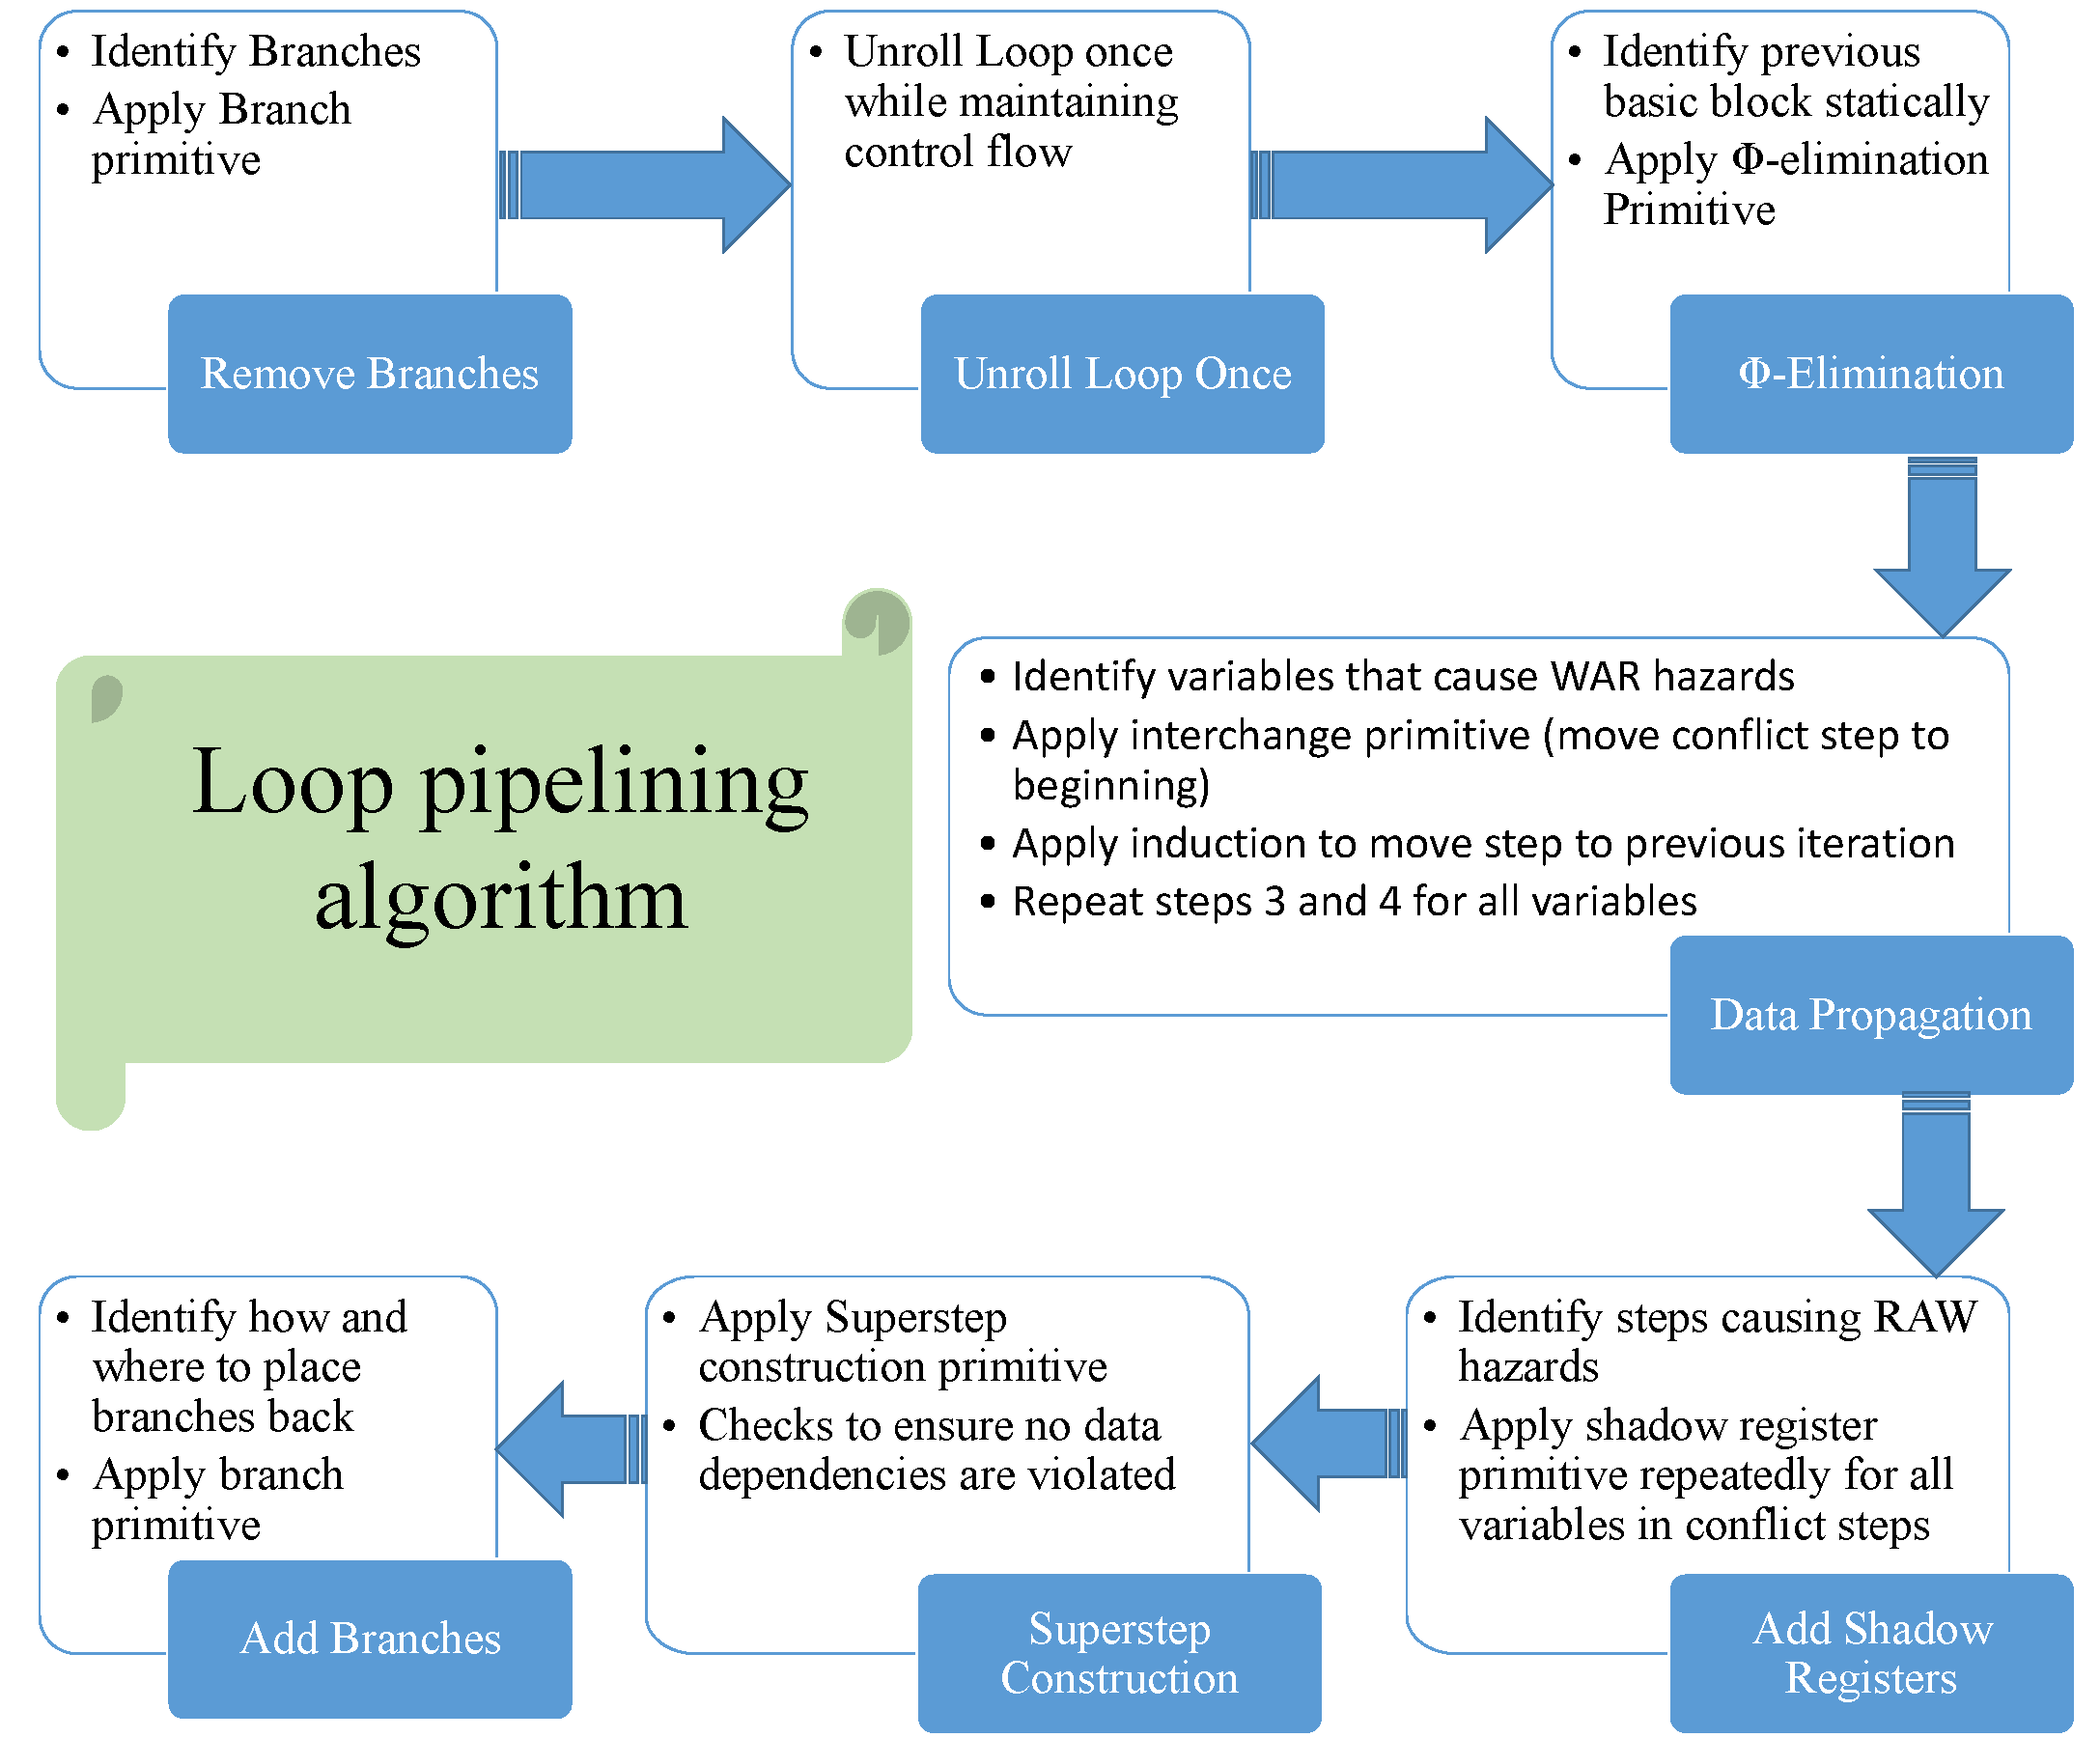
\includegraphics[width=5.5in]{fig-proposal/algorithm-using-primitives}
\end{tabular}
\end{center}
\caption{Our loop pipelining algorithm (built using primitives)}
\label{fig:algorithm-using-primitives}
\end{figure}

Given a sequential loop $S$ in CCDFG $C$ and pipeline interval $I$, we can create a pipelined loop $P$ using Algorithm~\ref{algo:loop}. Note that every step of the algorithm is built from ground up using our framework of provable primitives such that the algorithm can be certified by theorem proving. A quick overview of primitives used in the algorithm at each step are shown in Figure~\ref{fig:algorithm-using-primitives}.

\begin{algorithm}[H]
\caption{Pipelining algorithm}
\label{algo:loop}
\begin{algorithmic}[1]
\Procedure{PipelineLoop}{S, I}
\State $S_1 \leftarrow RemoveBranches(S)$
\State $S_2 \leftarrow UnrollLoopOnce(S_1)$
\State $S_3 \leftarrow \phi-Elimination (S_2) $.
\State $S_4 \leftarrow DataPropagation (S_3, I) $.
\State $S_5 \leftarrow GenerateShadowRegisters (S_4, I) $.
\State $ S_6 \leftarrow SuperstepConstruction (S_5, I) $.
\State $P \leftarrow AddBranches (S_6) $
\State \textbf{return} $(P)$.
\EndProcedure
\end{algorithmic}
\end{algorithm}

Now, we describe the steps to convert a sequential loop CCDFG (c.f. Figure~\ref{fig:algo1-1}) to a pipelined loop CCDFG in detail:

\begin{figure}[H]
\begin{center}
\begin{tabular}{c}
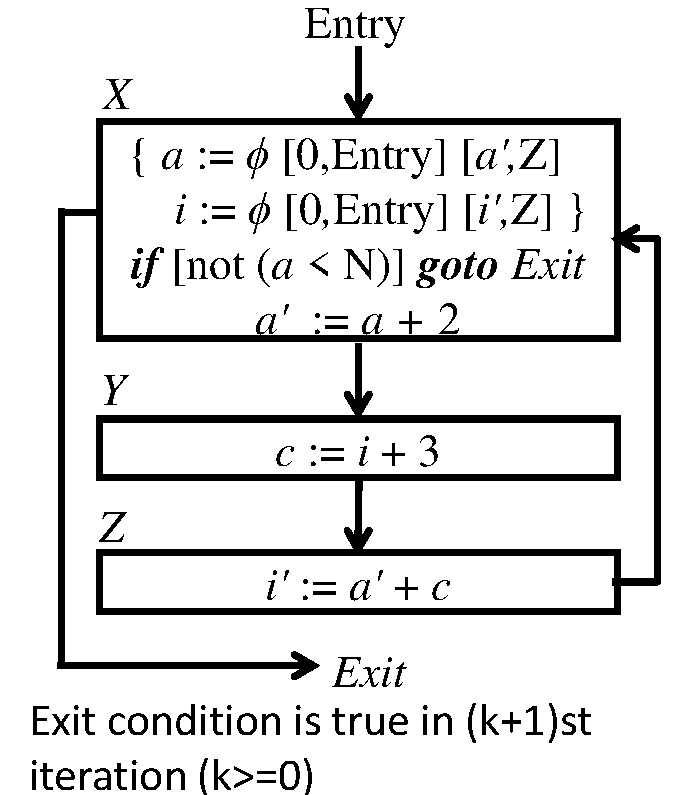
\includegraphics[height=3.1in]{fig-proposal/seq-ccdfg}
\end{tabular}
\end{center}
\caption{Sequential CCDFG with conditional branch}
\label{fig:algo1-1}
\end{figure}
 
{\bf Remove Branches}: We apply the branch primitive on $S$ (c.f. Figure~\ref{fig:algo1-1}) to remove the conditional and unconditional branch by explicitly defining the control flow in $S$. The output is a sequence of two CCDFG's $S_{loop}$ and $S_{preExit}$ connected through an edge as shown in Figure~\ref{fig:algo1-2}.
Note, that $S_{loop}$ does not contain the conditional branch originally present in $S$.
Executing $S$ such that $S$ exits in the $(k+1)$st iteration is same as executing $S_{loop}$ $k$ times
followed by $S_{preExit}$. This is possible because the input CCDFG has only one conditional and one unconditional branch as per our definition of pipelinable well formed CCDFG's.


\begin{figure}[H]
\begin{center}
\begin{tabular}{c}
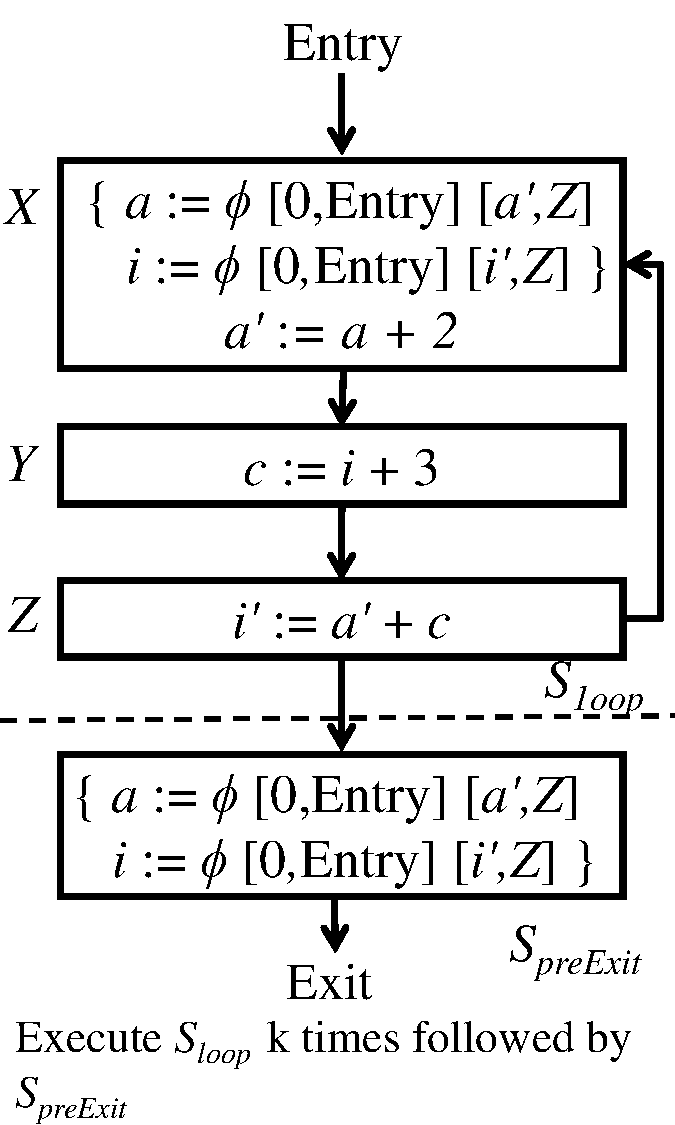
\includegraphics[height=3.45in]{fig-proposal/algorithm-after-removing-branches}
\end{tabular}
\end{center}
\caption{Sequential CCDFG without conditional branch. Note the addition of $S_{preExit}$ to explicitely define the control flow}
\label{fig:algo1-2}
\end{figure}

{\bf Unroll Loop Once}: We have already established that the first iteration behaves differently than the rest of the
iterations due to $\phi$-construct. So, in this particular step, we simply unroll the loop $S_{loop}$ once. This step does not use any primitive. It is an intuitively correct step, although we also formally verify it using induction in the final proof. We call the first iteration
$S_{pre}$ as shown in Figure~\ref{fig:algo1-3}(a).

\begin{figure}[H]
\begin{center}
\begin{tabular}{cc}
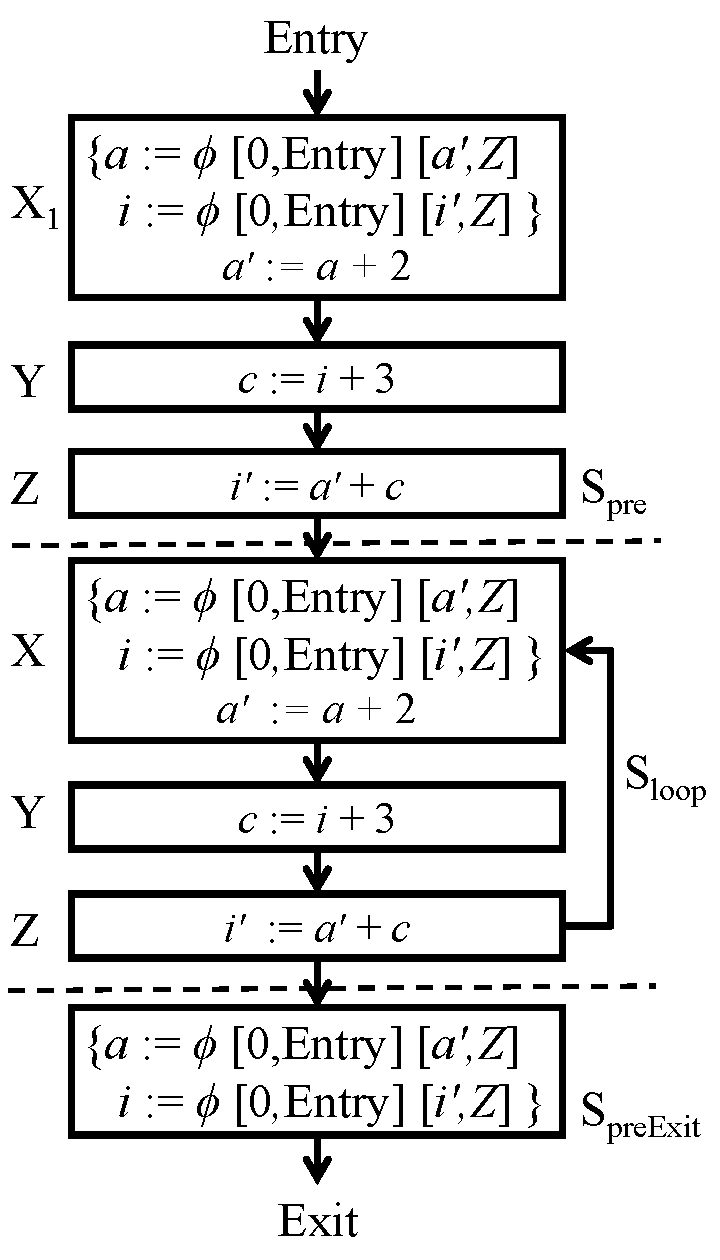
\includegraphics[height=4.5in]{fig-proposal/algorithm-two-iterations}
&
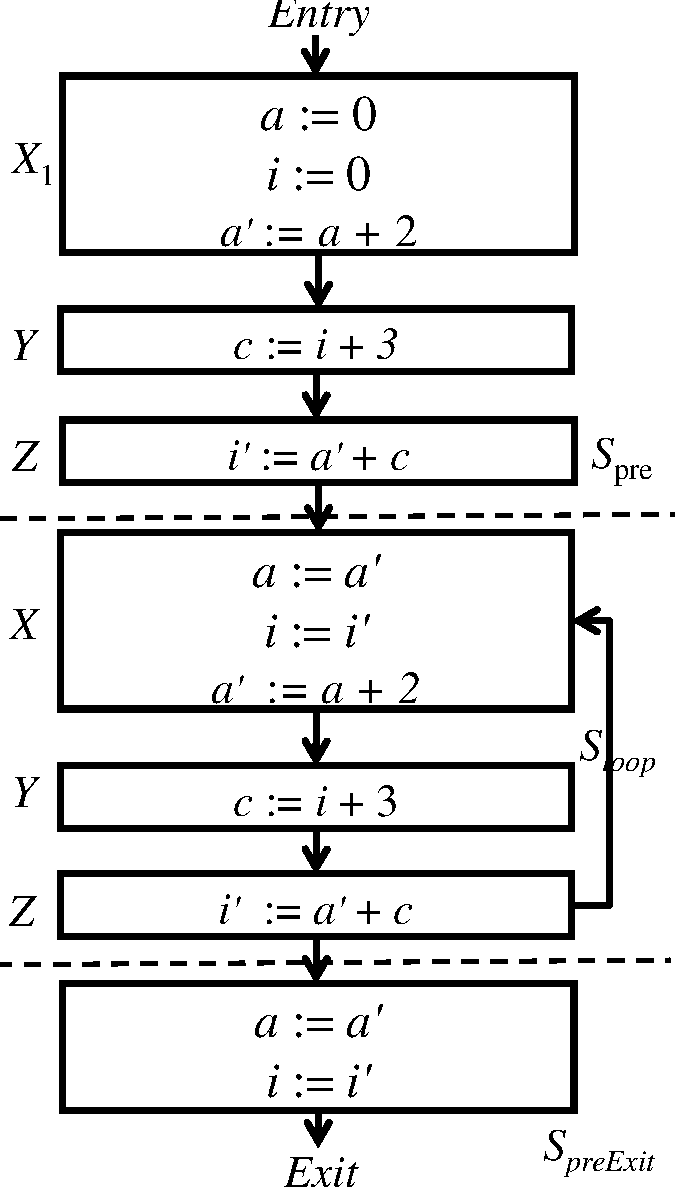
\includegraphics[height=4.5in]{fig-proposal/algorithm-after-phi-removal}
\\
(a) & (b)
\\
\end{tabular}
\end{center}
\caption{(a) Unrolling the loop once to separate the first iteration (b) After $\phi$-removal transformation}
\label{fig:algo1-3}
\end{figure}


{\bf $\phi$-elimination}: We apply the $\phi$-elimination primitive on $S_{pre}$, $S_{loop}$ and $S_{preExit}$ to return a CCDFG in which all the $\phi$-statements have been replaced with their corresponding assignment statements. Figure~\ref{fig:algo1-3}(b) shows the CCDFG after applying the $\phi$-elimination primitive. Note that $\phi$-construct is only in the first scheduling step of any iteration, so the remaining scheduling steps are the same in all the iterations.

\begin{algorithm}[t!]
\caption{Data propagation} 
\label{algo:data-propagation}
\begin{algorithmic}[1]
\Procedure{DataPropogration}{$L$}
\State $msteps \leftarrow GetLoopCarriedDependencies(L)$
\For {\textbf{each} mstep \textbf{in} msteps}
\If {$CheckConflict (L, mstep, N, I) \neq 0$}
\State $L \leftarrow RelocateMStep (L, mstep)$
\EndIf
\EndFor
\State \textbf{return} $(L)$
\EndProcedure
\end{algorithmic}
\end{algorithm}

{\bf Data propagation:} Algorithm~\ref{algo:data-propagation} describes how to compute candidates for data
propagation across pipeline iterations. It is a critical step in removing data hazards. We want to make sure that when we pipeline a loop, we do not read a variable which has not
yet been written. A critical observation is that data propagation is required only for loop carried dependencies.
$GetLoopCarriedDependencies$ identifies the microsteps where loop carried dependencies are being read. Then,
$CheckConflict$ checks whether there would be a conflict when we pipeline the loop.
Conflict occurs when the value being read in a microstep is not yet written in the pipelined loop execution. If so, $RelocateMSteps$ works in two steps. It first relocates the microstep which reads the variable in an iteration to the starting of $S_{loop}$. This step can be proved by the interchange primitive since we have already established that the value has not been written yet so there are no read write hazards in between. In the next step, we relocate the microstep to the end of $S_{loop}$. Note, to maintain the invariant that executing CCDFG before and after this relocation is the same, we need to add the microstep at the end of $S_{pre}$ as well and remove it from $S_{preExit}$. This step ensures that any variable which is being read has already been written. Note that in order to maintain the invariant, only those microsteps can be propagated which exist in $S_{preExit}$, which means only those steps which occur before the conditional branch in original CCDFG can be relocated. This ensures that our algorithm does not have the bug which the previously proposed algorithm had.
In Figure~\ref{fig:algo1-3}(b) we found that the loop carried dependency $i'$ in $X$ would create a conflict when we would move $X$ before $Z$ while pipelining. So, first we relocate the microstep $i := i'$ to the beginning of $S_{loop}$ using interchange primitive in Figure~\ref{fig:algo2-2}(a). Then, we move the microstep to end of $S_{pre}$ and $S_{loop}$ and remove the microstep from $S_{preExit}$ in  Figure~\ref{fig:algo2-2}(b). Note that this preserves execution as explained more in Chapter~\ref{sec:proof}. 
This step needs to be repeated for every variable found using $GetLoopCarriedDependencies$.

\begin{figure}[t!]
\begin{center}
\begin{tabular}{cc}
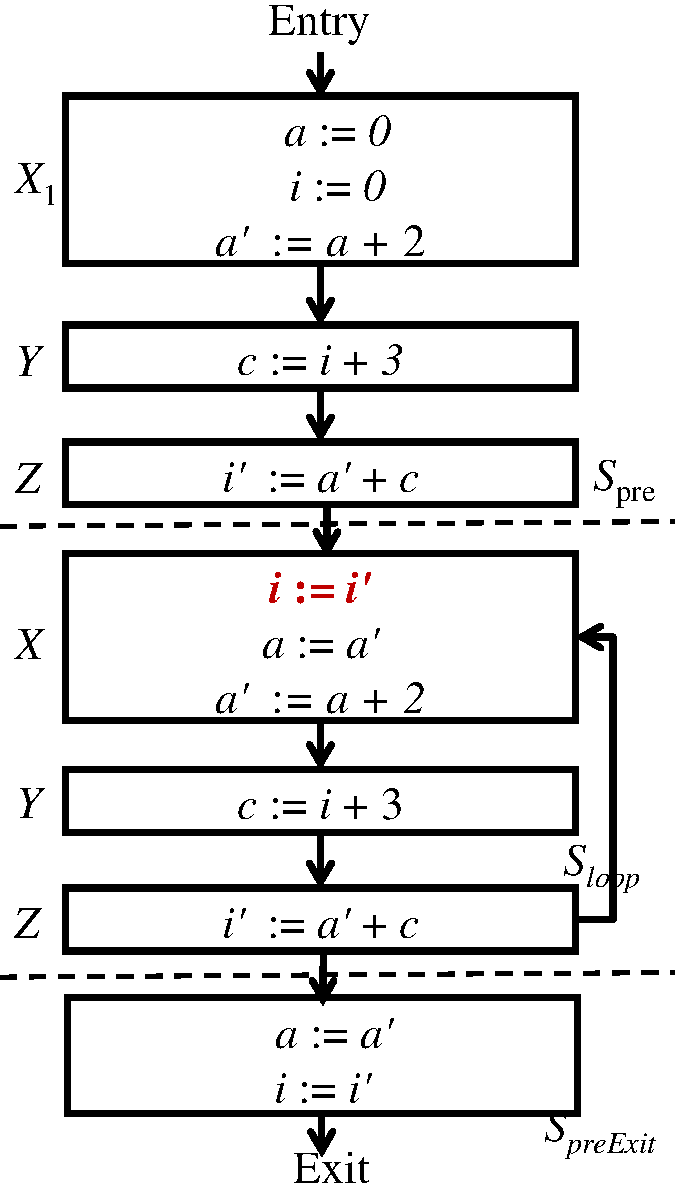
\includegraphics[height=4.5in]{fig-proposal/algorithm-after-data-propagation-1}
&
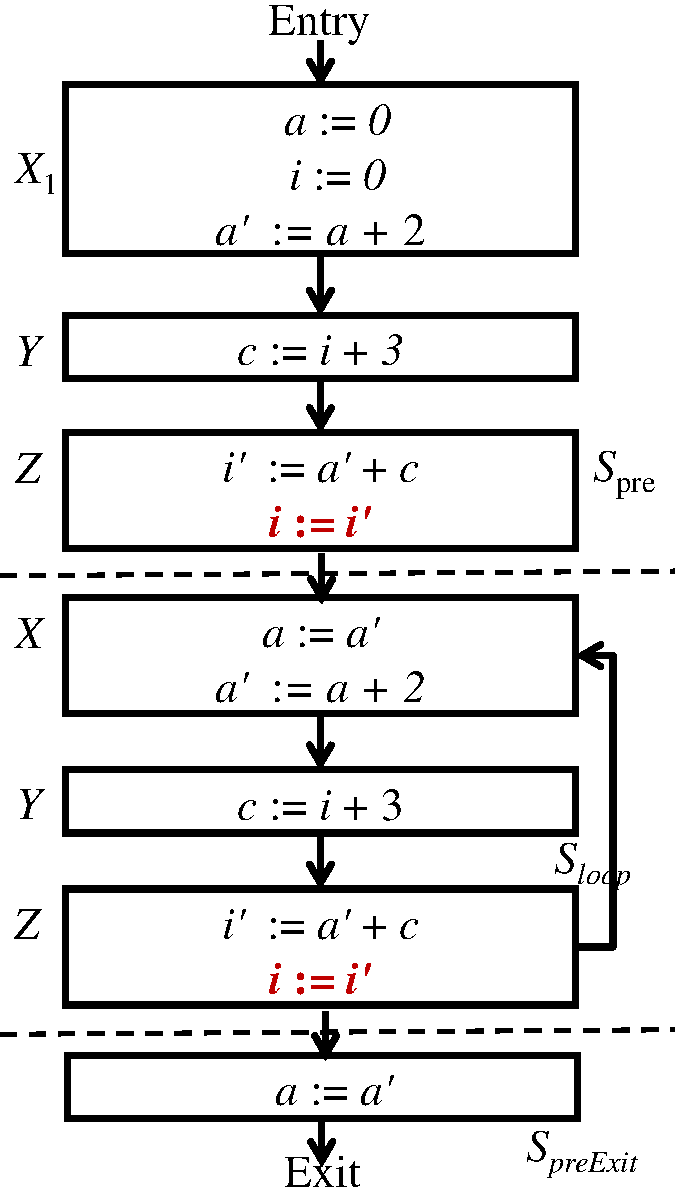
\includegraphics[height=4.5in]{fig-proposal/algorithm-after-data-propagation-2}
\\
(a) & (b)
\\
\end{tabular}
\end{center}
\caption{(a) Data propagation - first step (b) Data propagation - second step}
\label{fig:algo2-2}
\end{figure}

{\bf Generate shadow registers:} Algorithm~\ref{algo:generate-pipeline-registers} inserts shadow registers
to prevent variables from being overwritten before being read. 

\begin{algorithm}[H]
\caption{Generate shadow registers} 
\label{algo:generate-pipeline-registers}
\begin{algorithmic}[1]
\Procedure{GenerateShadowRegisters}{$L$, $I$}
\State $V \leftarrow GetAllVariables(L)$.
\For {\textbf{each} v \textbf{in} V}
\State $w_v \leftarrow WriteVariable (v, L)$.
\State $r_v \leftarrow LastReadVariable (v, L)$.
\If {$RequireShadowRegister (r_v, w_v, I) \neq 0$}
\State $L \leftarrow AddShadowRegister (w_v, L)$.
\EndIf
\EndFor
\State \textbf{return} $(L)$.
\EndProcedure
\end{algorithmic}
\end{algorithm}

We first compute all program variables that may be
overwritten before being read, which means these are the variables that require shadow registers. To find such variables,
 $GetAllVariables$ first gets a set of all variables. Then, for each variable, we compare the distance (the number of scheduling steps) between the write of
  the variable $w_v$ $(WriteVariable)$ and the last read of the variable $r_v$ $(LastReadVariable)$ in an iteration; if the
   distance is greater than $I$ (pipeline interval), the variable is assigned the new data value of the next iteration before the current iteration's value
    has been fully consumed; this warrants insertion of shadow registers in every scheduling step between the $r_v$ and $w_v$. The value is propagated every clock cycle following the CCDFG data flow.
We apply the shadow register primitive on the microstep which writes the variable $(AddShadowRegister)$. We assign that
 variable to a new temporary variable called shadow register in every new scheduling step and replace all subsequent reads of that variable with the shadow register till its next write. In Figure~\ref{fig:algo3-1}, we introduce a shadow register $a\_reg$ in $X$ and $a\_reg2$ in $Y$. This step is also repeated for all the variables found using $GetAllVariables$.



\begin{figure}[t!]
\begin{center}
\begin{tabular}{c}
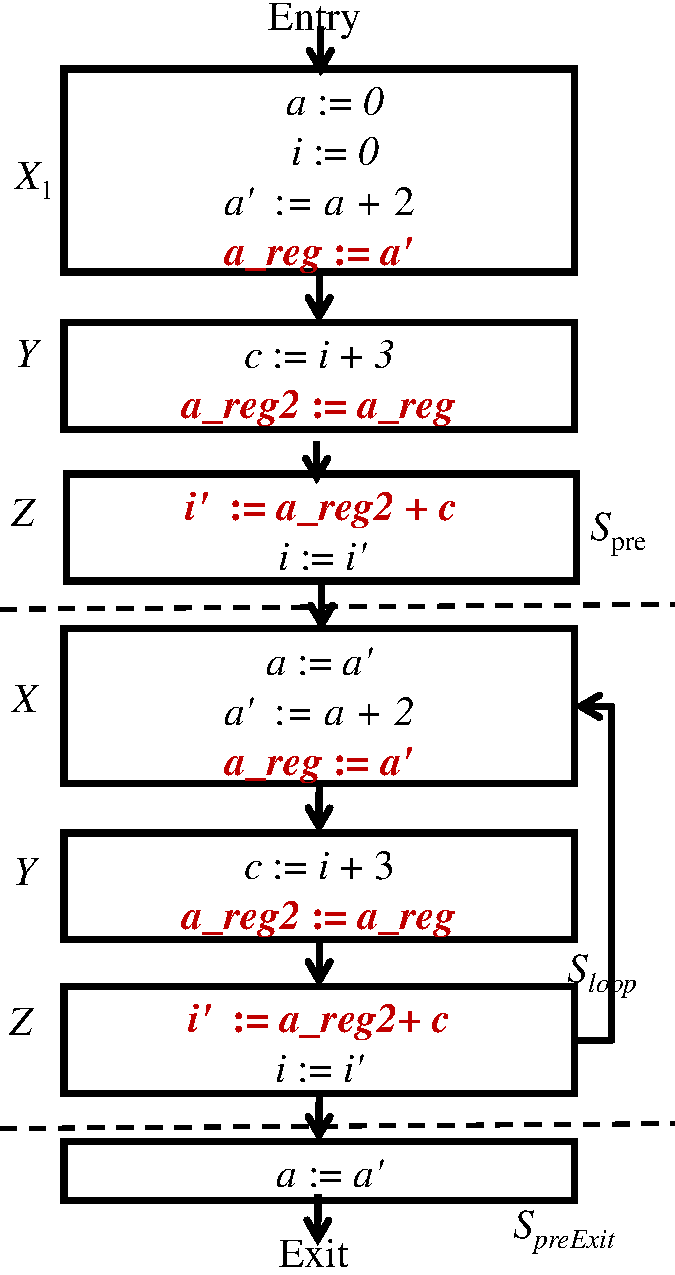
\includegraphics[height=5in]{fig-proposal/algorithm-after-shadow-register}
\end{tabular}
\end{center}
\caption{After shadow register}
\label{fig:algo3-1}
\end{figure}

\begin{figure}[t!]
\begin{center}
\begin{tabular}{c}
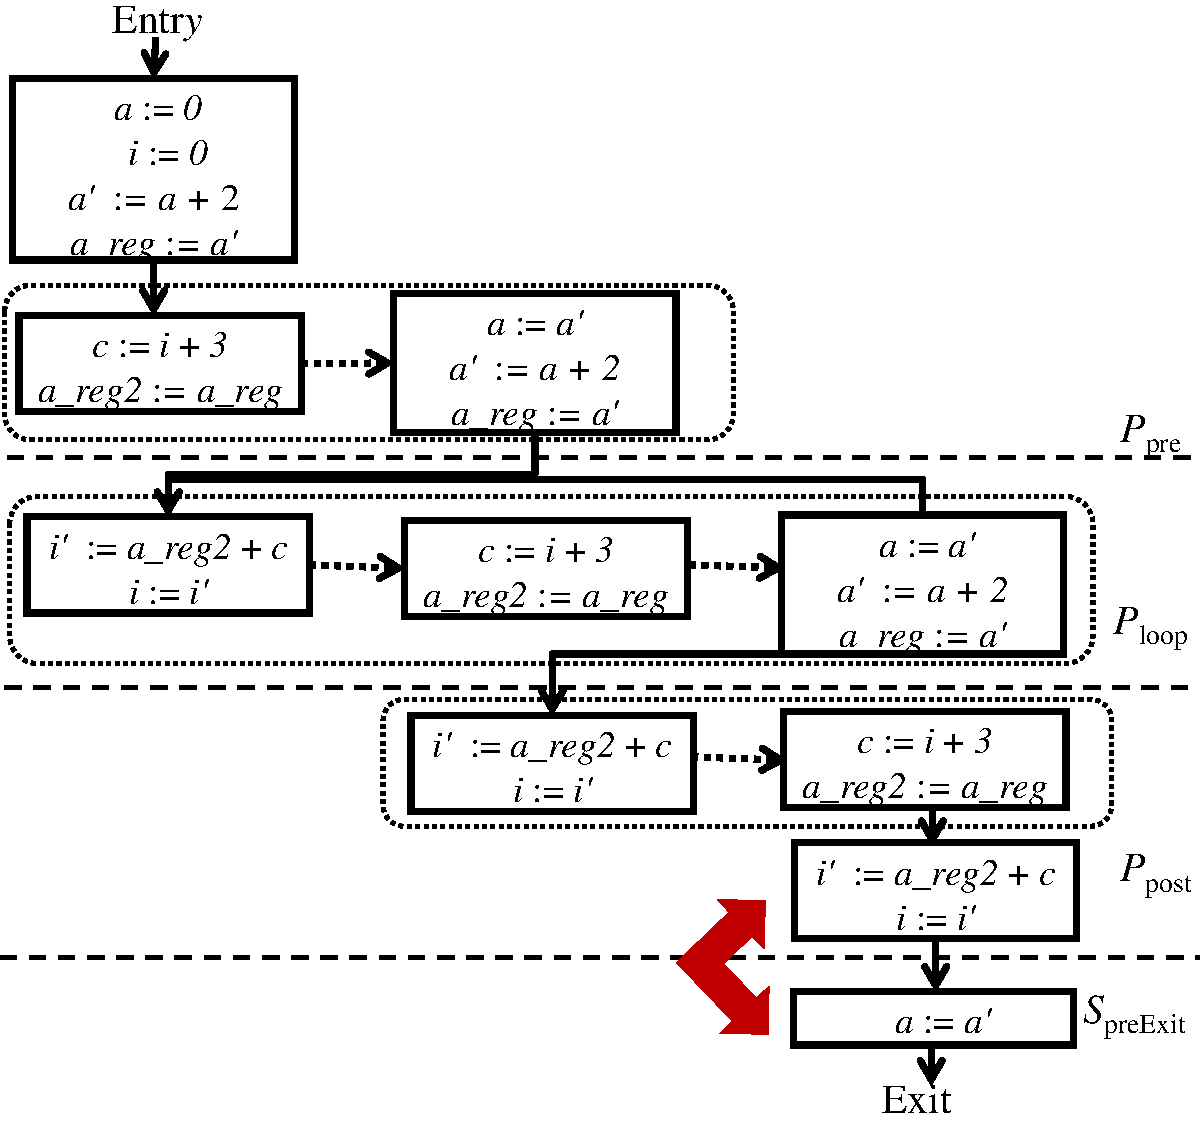
\includegraphics[width=5.5in]{fig-proposal/algorithm-after-superstep-construction}
\end{tabular}
\end{center}
\caption{After superstep construction}
\label{fig:algo3-2}
\end{figure}

{\bf Superstep construction:} Now that we have removed the data hazards, we can successfully pipeline the loop using  the pipeline interval $I$. We combine the scheduling steps of the successive iterations, forming scheduling ``supersteps'' that act as scheduling steps for the pipelined
implementation. Supersteps must account for read-after-write hazards, i.e., if a variable is written in a scheduling step $s$ and read subsequently in $s'$ then $s'$ cannot be in a superstep that precedes $s$ in the control/data flow. A scheduling step is allowed to move up another scheduling step only if there are no intermediate read and write conflicts. Note that we implement data forwarding; thus $s$ and $s'$ can be in a single scheduling superstep.
Superstep construction on $S_{pre}$ and $S_{loop}$ creates a CCDFG with three parts: prologue $P_{pre}$, $P_{loop}$ which is the full pipeline stage and epilogue $P_{post}$ as shown in Figure~\ref{fig:algo3-2}. We will later prove using our invariant that executing $P_{pre}$ followed by $k$ iterations of $P_{loop}$ followed by $P_{post}$ is equivalent to executing $S_{pre}$ followed by $x$ iterations of $S_{loop}$, where value of $x$ is determined based on value of $k$, pipeline interval $I$ and number of scheduling steps in $S$.

\begin{figure}[t!]
\begin{center}
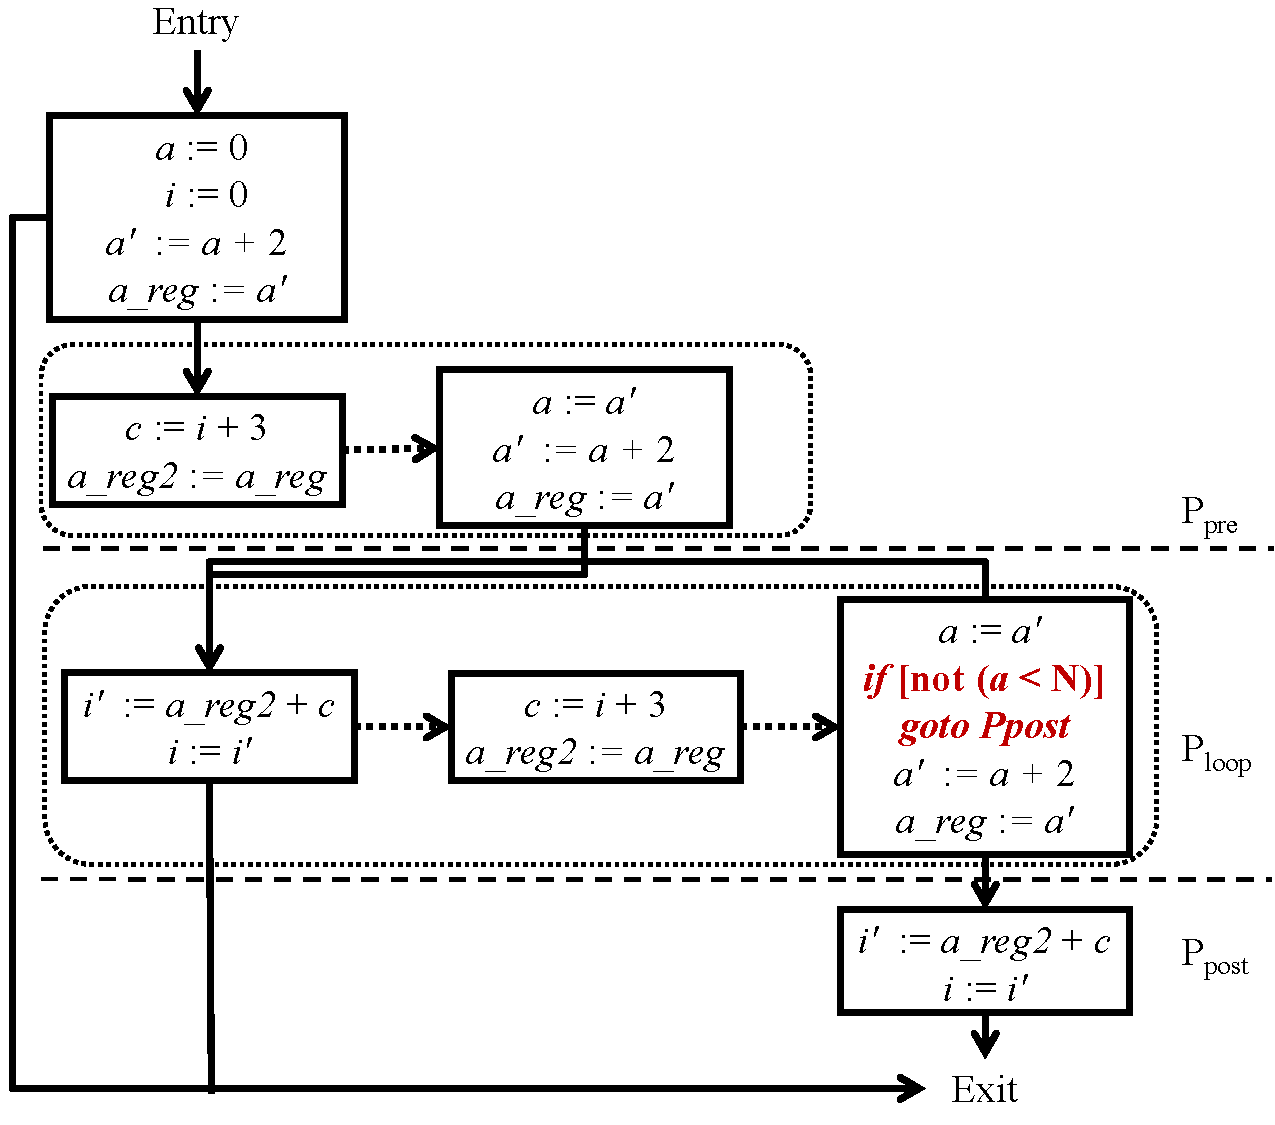
\includegraphics[width=5.5in]{fig-proposal/algorithm-after-adding-branches}
\end{center}
\caption{Final pipelined CCDFG}
\label{fig:algo4}
\end{figure}

{\bf Add Branches:}  To add the branches back, we use the a combination of interchange primitive and reverse of Branch primitive. Note in Figure~\ref{fig:algo3-2}, if there are no read write hazards in between the last scheduling step $Z$ of $P_{post}$ and $S_{preExit}$, we can interchange them using interchange primtive. Now recall from the branch primitive that if there is a loop structure $S_{loop}$ with a conditional branch, then executing $S_{loop}$ such that it exits in the (k+1)st iteration is same as executing $S_{loop}$ without the conditional branch followed by only those steps from $S_{loop}$ which occur before the branch $S_{preExit}$. Now, we apply the reverse of branch primitive here. $P_{loop}$ in Figure~\ref{fig:algo3-2} is a loop structure without a conditional branch, followed by a collection of microsteps $P_{preExit}$ (here, a collection of $Z$, $Y$ and $S_{preExit}$). Then, we can add an exit conditional branch in $P_{loop}$ after the microsteps $P_{preExit}$. This branch points to the next scheduling step after the loop $P_{post}$ if the exit condition is true. We can add the conditional and the unconditional branch as shown in  Figure~\ref{fig:algo4}.  

We now have the final pipelined loop structure. We describe a proof sketch for the primitives and the algorithm in the next chapter.

%Next we discuss an outline of the proof of our algorithm using theorem proving. 
    \ifoddchapterpage
    \newoddpage
    \fi

    %%-------------------------------------------------------------------------
    \chapter{Proof Sketch}
\label{sec:proof}

Certification of our loop pipelining algorithm naturally requires a certification of each of our primitives.
In addition, we need to ensure that every time a primitive needs to be applied, the conditions
under which the primitive can be applied are maintained. We discuss both aspects below.

\section{Correctness of Primitives}
We must prove that applying a particular primitive is correct, {\em i.e.},
maintaining a certain invariant. This is proven without
considering how it is applied in the context of a pipeline
synthesis algorithm. We give an outline of the proof to justify that the primitives are correct.

{\bf $\phi$-elimination primitive:} We prove that the execution
  of a $\phi$-construct is the same as executing the corresponding
  assignment statements. Note that this is not trivial since
  given a microstep in a scheduling step containing the
  $\phi$-construct, the algorithm has to use static analysis
  to deduce the previous scheduling step.

{\bf Shadow register primitive:} We prove that adding
  a shadow register microstep $x\_reg = x$ does not change the
  value of any variable except the shadow variable. Also, we
  prove that now since value of $x\_reg$ would be equal to value
  of $x$, executing a statement which reads $x$ has the same
  effect on the state as executing a statement which reads
  $x\_reg$ till the next write of $x$. We
  determine the variables read and written in a statement by
  analyzing the execution semantics. Note that $x\_reg$ has to be a new variable which
  is neither written nor read in the given statements.

{\bf Interchange primitive:} We prove that we can interchange two scheduling steps which do not have
  read-write conflict. Given an initial state, the state after
  executing scheduling steps $m$ and $n$ is the same as the state after
  executing $n$ then $m$ if $m$ and $n$ have no read-write
  conflict. Suppose, the state after
  executing $m$ and $n$ is $s_1$ and that after executing $n$ and
  $m$ is $s_2$. We prove that for any variable $x$, its
  value remains same in $s_1$ and $s_2$. After normalizing
  the states, we can prove that $s_1$ is equal to $s_2$, i.e.,
  the states are the same after executing the two scheduling steps in
  a sequence or in an interchanged order. Again, reasoning about read and
  write of statements involves reasoning about execution
  semantics of all types of microsteps present in the
  language which is not trivial.

{\bf Branch primitive:} The proof of the primitive follows from the definition of branch primtive itself as explained in Section 5. This proof would involve semantically analyzing the branch statements and induction on the steps of the CCDFG. 

{\bf Superstep construction primitive:} This primitive is proved
using the interchange primitive and our key invariant described in detail below.

\section{Key Invariant on Correspondence Between Back-edges of Sequential and Pipelined Loops}
 Our key invariant defines a ``correspondence relation''
between the back-edges of the sequential and pipelined CCDFGs.
The relation can be informally paraphrased as
follows~\cite{disha-itp14}.

\begin{quote}
Let $S$ be a sequential loop and $P$ be the pipelined loop
generated from our algorithm. The pipelined loop after superstep construction
consists of
three stages before $S_{preExit}$ as depicted in
Figure~\ref{fig:algo3}(b): prologue $P_{pre}$, full stage
$P_{loop}$, and epilogue $P_{post}$.  Let $s_l$ be any state of $P$
poised to execute $P_{loop}$, and let $k$ be any number such that
the loop of $P$ is not exited in $k$ iterations from $s_l$.
Then executing $P_{pre}$ followed by $k$ iterations of $P_{loop}$ is
equivalent to executing first iteration of $S$, say $S_1$
followed by $(k - 1)$ iterations of $S$ together with a
collection of ``partially completed'' iterations of
$S$.\footnote{The formalization actually characterizes each
  incomplete iteration, \eg, if the pipeline includes $d$
  iterations and successive iterations are introduced in
  consecutive clock cycles, then the $i$-th iteration has $i
  - 1$ incomplete scheduling steps.}
\end{quote}

The partially completed iterations can be determined by the
length of the first iteration in $P_{pre}$ and the pipeline interval.
Suppose the length of the first iteration in $P_{pre}$
is {\tt m} and the pipeline interval is {\tt i}. Note that we
can calculate the value of {\tt m} based on the number of scheduling steps in a CCDFG
and the pipeline interval. The partially completed iterations mean $m$
scheduling steps of $S$ followed by $(m-i)$ scheduling steps of $S$, by
$(m-2i)$ scheduling steps of $S$, etc. while $(m-ni)$ is positive.

In our example, {\tt m} is $2$
and {\tt i} is $1$.  The invariant implies that starting
from the same initial state, executing $P_{pre}$ and {\tt k}
iterations of $P_{loop}$ is the same as executing {\em k}
iterations of $S$, followed by $m = 2$ scheduling steps of
$S$, followed by $ (m - i) = 1$ scheduling steps of $S$.

As is standard with proofs involving invariants, there are
two obligations to prove the correctness, \viz, that it is indeed
an invariant, and that its invariance is sufficient to imply
the desired correctness theorem.  Here we give a sense of
our envisioned proof.

Our invariant is defined specifically to make the proof
sufficiency straightforward.
Equivalence of CCDFG states of $P$ and $S$ follows from the
invariant by noting that the epilogue $P_{post}$ exactly
constitutes the incomplete scheduling steps of $S$ specified
by the invariant
(cf. Figure~\ref{fig:invariant-implies-correctness}).

\begin{figure}[t!]
\begin{center}
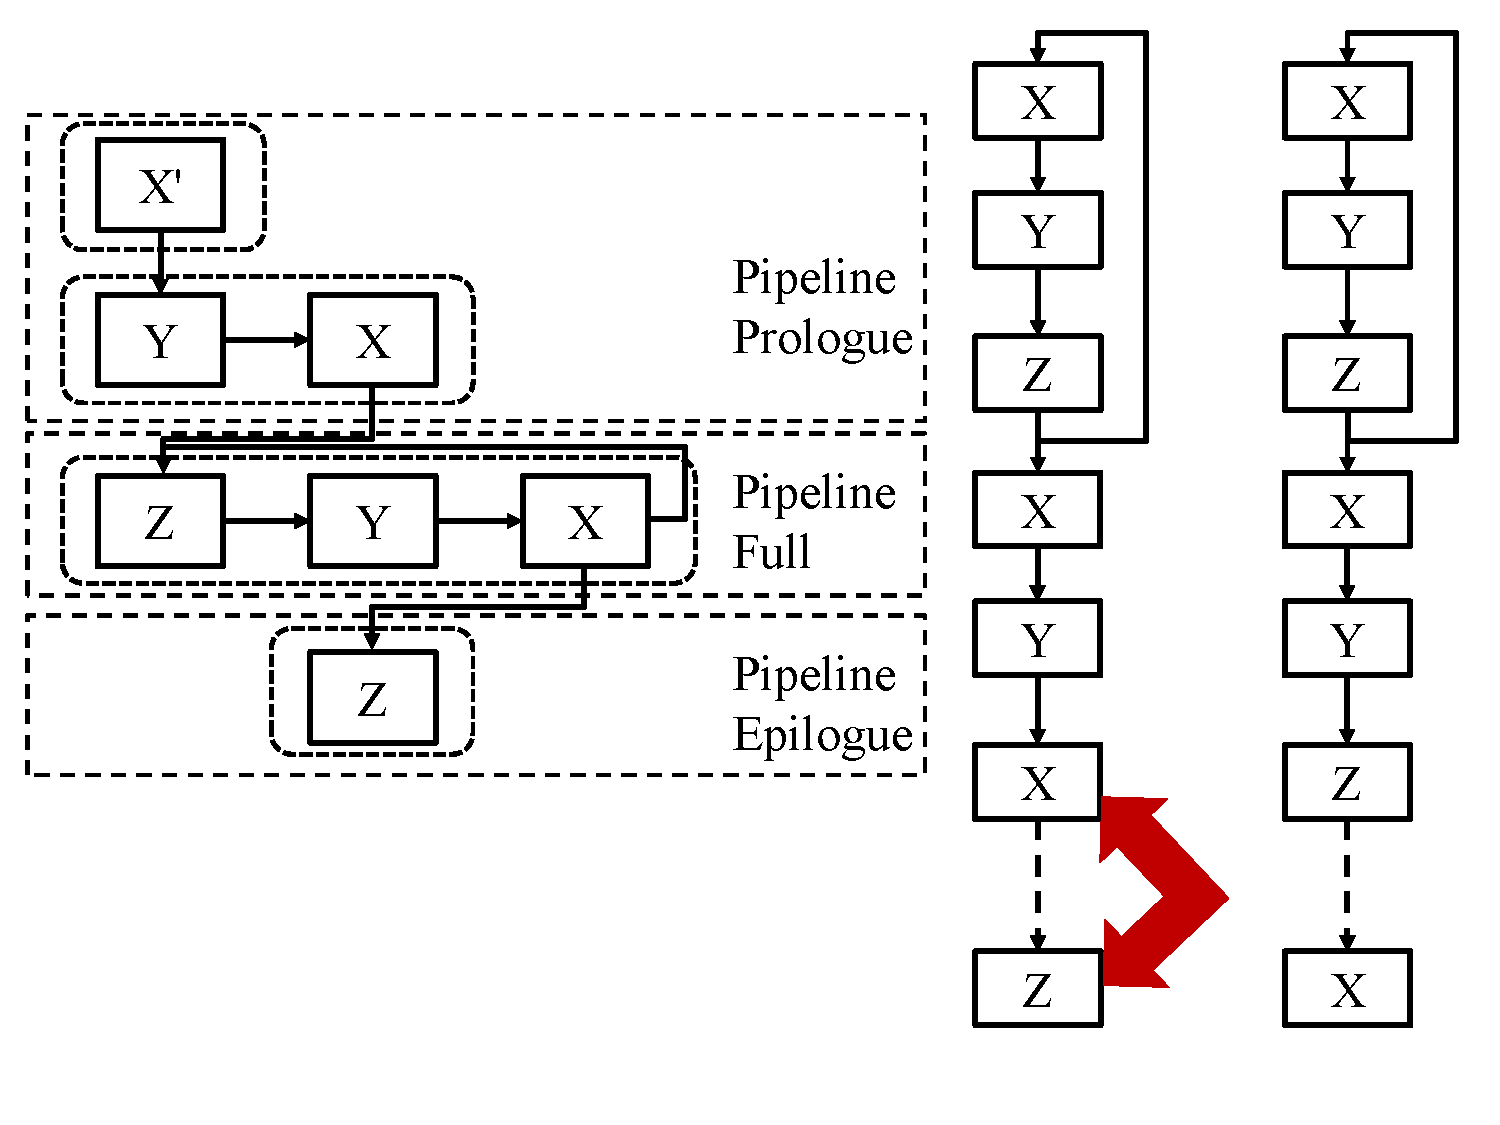
\includegraphics[height=2.2in]{fig-proposal/invariant-implies-correctness}
\end{center}
\caption{Correctness of invariant implies the correctness statement}
\label{fig:invariant-implies-correctness}
\end{figure}

The proof of invariance of this predicate is, of course, the
main ``work horse'' in this exercise.  The proof depends on
our interchange primitive which in turn is based on a fundamental idea for pipelining,
\viz, commutability of
independent instructions.

\begin{quote}
Suppose that the
set of variables written and read by two consecutive
operations $a$ and $b$ is disjoint.  Then executing $a$
followed by $b$ generates the same result as executing $b$
followed by $a$.
\end{quote}

If we view the scheduling steps in
Figure~\ref{fig:high-level-synthesis} as arranged in a
matrix, then the sequential execution proceeds column-wise
along the matrix while the pipelined execution proceeds
row-wise.  Thus the core proof obligation involves the
following two proof requirements.

\begin{enumerate}[--]
\item Our pipelining algorithm correctly combines the
  ``appropriate'' scheduling supersteps which do not have
  read-write hazards.
\item Given that there are no read-write hazards at
  appropriate places, executing scheduling steps row-wise is
  same as executing those scheduling steps column-wise in
  the pipelined CCDFG.  This requires the use of interchange primitive.
\end{enumerate}

\begin{figure}[t!]
\begin{center}
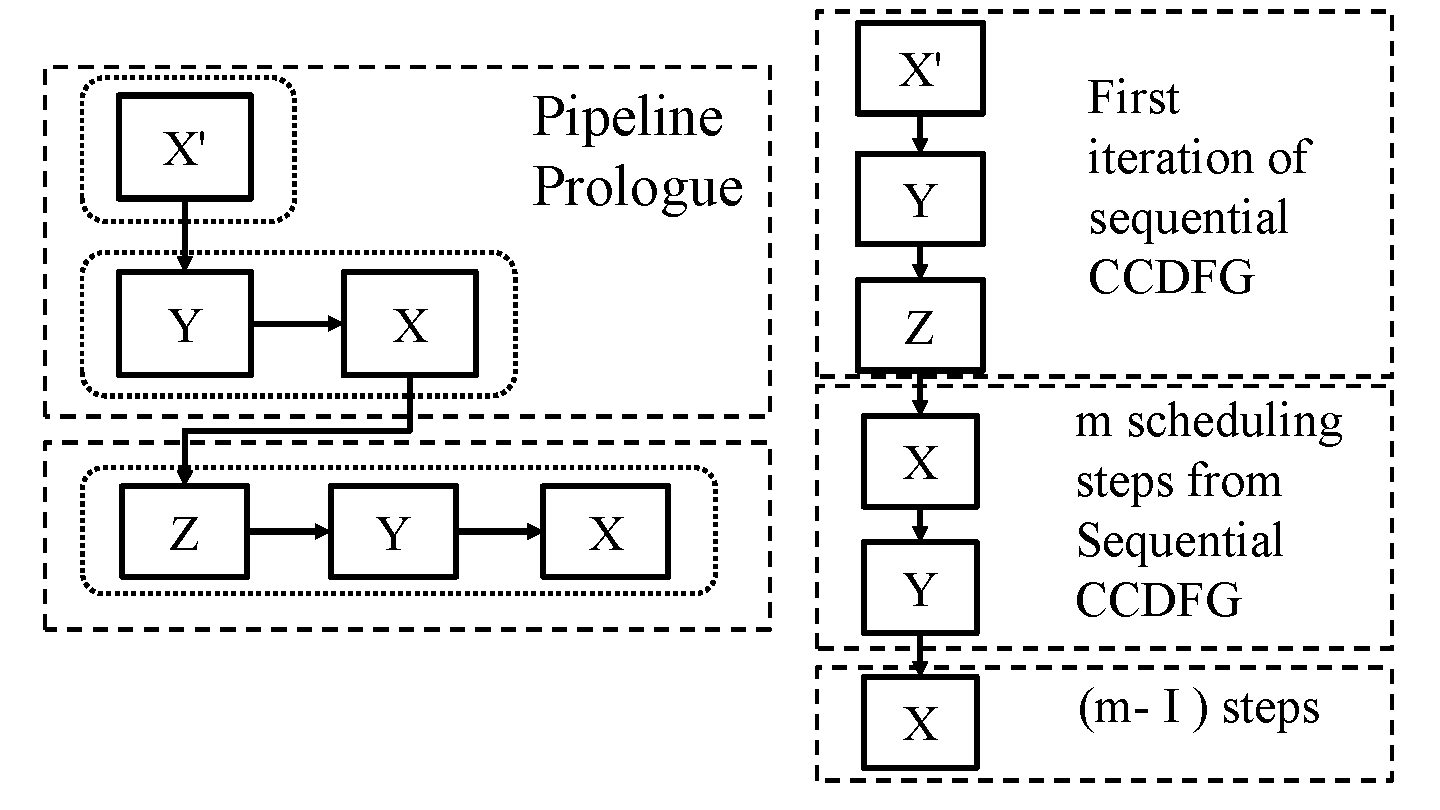
\includegraphics[width=3.5in]{fig-proposal/invariant-base-case}
\end{center}
\caption{Invariant base case where $k = 1$, executing
  pipeline prologue and one pipeline full stage is the same
  as executing $S_{pre}$ followed by a sequence of partially
  completed sequential loop CCDFG.}
\label{fig:invariant-base-case}
\end{figure}

\begin{figure}[t!]
\begin{center}
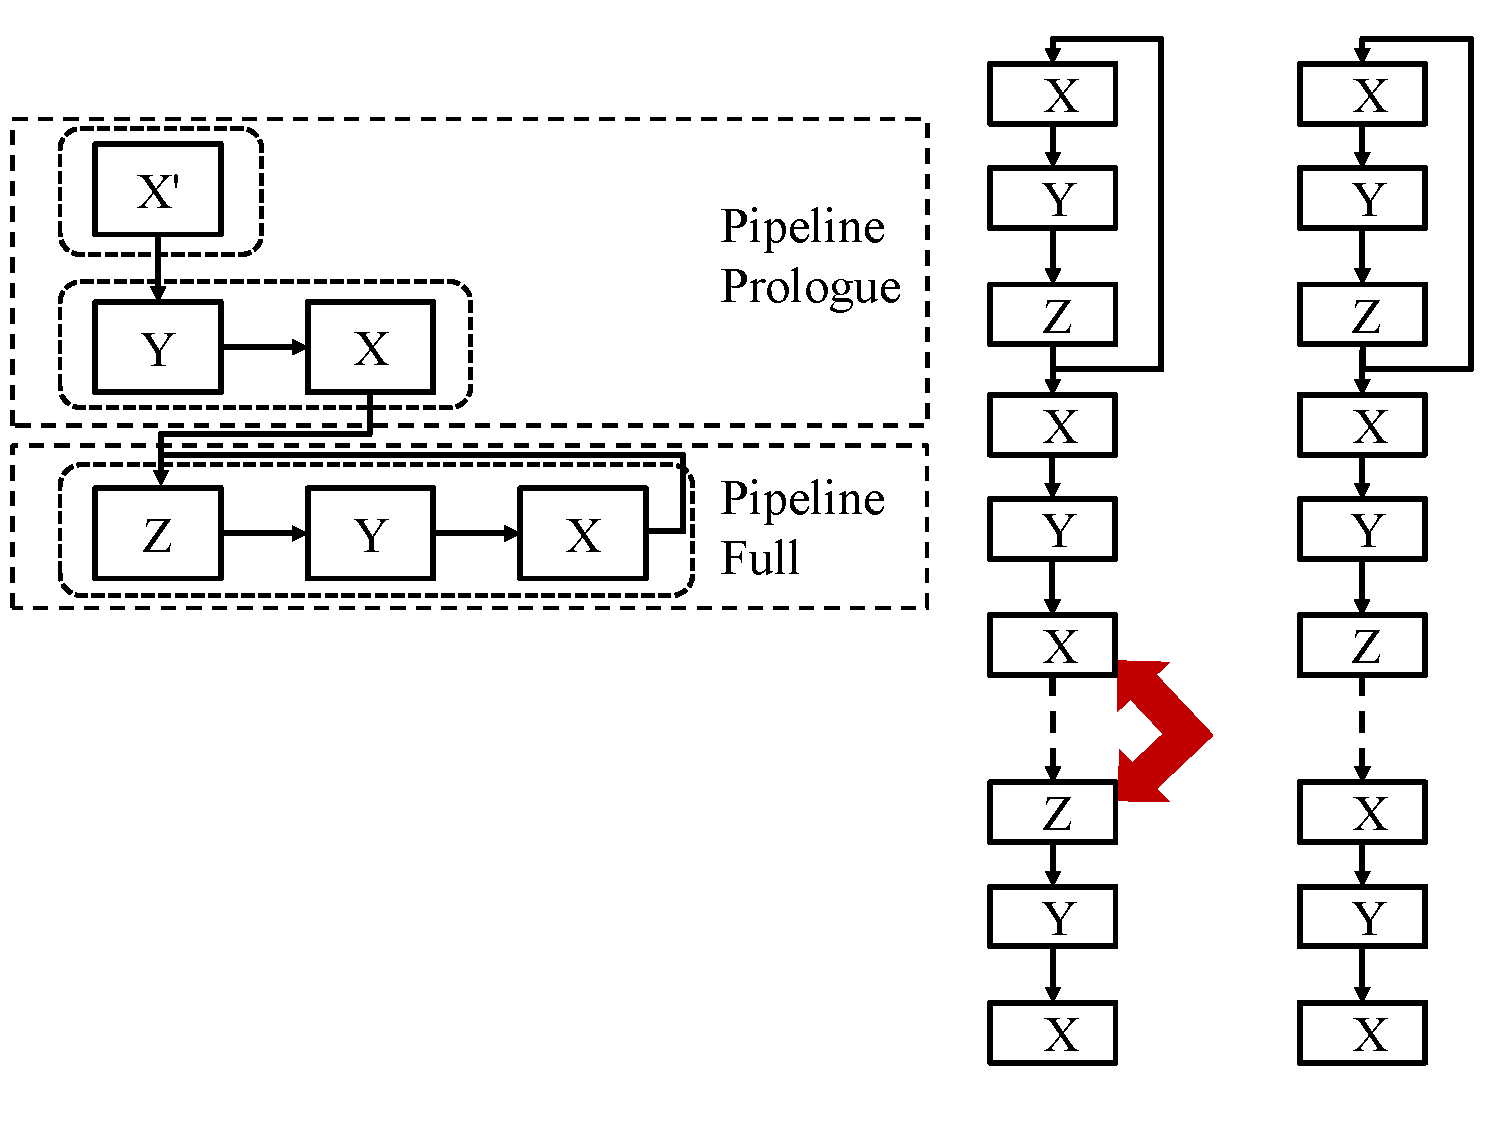
\includegraphics[height=2.2in]{fig-proposal/invariant-inductive-step}
\end{center}
\caption{Assuming that
  invariant is true for $k$ steps, executing one pipeline full
  stage on both sides gives us $(k + 1)$ iterations of
  sequantial loop CCDFG followed by partially completed
  sequences as expected.}
\label{fig:invariant-inductive-step}
\end{figure}

Although these requirements justify that our correspondence
relation is an invariant, they are used somewhat differently
in the base case (when the number of iterations $k$ of the
pipelined loop is $1$) and inductive step (assume the
invariant holds for $k$ iterations of the pipeline and prove
that it holds for $(k+ 1)$ iterations).  Their usage is
pictorially shown in Figures~\ref{fig:invariant-base-case}
and~\ref{fig:invariant-inductive-step}.  For
the base case, we commute operations in the loop prologue of
the pipeline (which corresponds to the first iteration after
unrolling) with the loop body, while for the inductive step
we work with two consecutive iterations of the loop.

Our invariant is very different from a typical invariant
used in the verification of pipelined machines (\eg, for
microprocessor pipelines).  We make explicit the
correspondence with the sequential execution.  The key
requirement from a pipeline invariant, \viz, hazard freedom,
is left implicit and arises indirectly as a proof obligation
for invariance of this predicate.  Most microprocessor
pipeline verification work went the other way.  For
instance, Sawada and Hunt's invariant~\cite{sh:pipeline},
expressed through an intermediate structure called MAETT,
``tracks'' the instructions as they pass through different
pipeline stages to ensure that hazards are not introduced.
One difference in our case is that we are not working with a
concrete pipeline with a fixed set of operations but an
algorithm that generates pipelines with an arbitrary
sequence of scheduling steps; a construction like MAETT is
thus not directly applicable.  However, there is a deeper
reason for defining our invariant the way we did.
Suppose we simply unroll the loop in the sequential
design three times, and then use a technique similar to
MAETT to track scheduling steps in this ``unrolled loop
body'' in the pipeline execution.  Unfortunately, this does
not work, because of the back edge.  There is no direct
correlation between this edge and any edge in the sequential
loop.  In fact, it is interesting to observe what its
introduction achieves: completion of one scheduling step in
each of the three partially executed, overlapping loop
iterations.  This suggests that the invariant must
explicitly capture the state of the executions that have
been partially completed during each iteration of the
pipeline ({\em ie}, each traversal of the back edge).


\section{Correctness of Our Algorithm}

The algorithm is essentially built from ground-up using primitives
as shown in Section~\ref{sec:pipelining-algorithm}. 
However, apart from proving correctness of each primitive and our key invariant,
we also need to ensure that the primitive is applied by our
algorithm properly, {\em i.e.}, the environment
assumptions on which the {\bf correctness of primitive}
depends are maintained appropriately by the algorithm at
the point where the primitive is applied. 
The correctness of each primitive discussed above, entails a
so-called ``assume-guarantee'' reasoning: the primitive is
guaranteed to maintain the desired invariant if and only if
it is applied under certain well-formed conditions.  To use
these correctness statements to verify the algorithm, we
must therefore prove that the algorithm applies each
primitive appropriately, maintaining the well-formedness
condition required for the correctness of the primitive.
Note that verifying this requires an inductive proof
relating the states of the CCDFG $C'$ generated after the
application of the transformation with the original CCDFG
$C$.  The induction is on the lengths of execution of $C$
and $C'$.  Note that the induction is non-trivial because
transformations have significant ``global'' effect on a
CCDFG.  These include one or more of the following:

\begin{enumerate}
\item Replacing one microstep of $C$ with more than one
  microsteps in $C'$ ({\em e.g.}, $\phi$-elimination), or
\item Interchanging scheduling steps ({\em e.g.},
  interchange), or
\item Changing the variable being read or written in several
  microsteps ({\em e.g.}, shadow register)
\end{enumerate}
The upshot is that an inductive theorem relating $C$ and
$C'$ must be strong enough to comprehend the global effects.
For instance, an inductive statement showing the
correctness of $\phi$-elimination must account for the fact
that the number of microsteps of $C$ is different from that
of $C'$.  Thus an execution of $C$ for $n$ microsteps must
correspond to an execution of $C'$ for a different number
$m$ of microsteps, where the number $m$ is a function of $n$
and the structures of $C$ and $C'$; the statement of the
correctness of $\phi$-elimination must characterize the
value of $m$ precisely, perhaps defining functions that
statically and symbolically execute $C$ and $C'$, in order
to be provable by induction.  Furthermore the functions so
introduced for static symbolic execution must themselves be
proven correct.

We can take each stage one by one to understand the complexity involved in 
verifying the algorithm as a whole over and above the verification of 
individual primitives. \textbf{Discusss with Sandip Sir, whether these things are worth mentioning and then elaborate}

In the $AddBranches$ stage, which is the first stage of pipelining algorithm, we 
have to create a correspondence between randomly executing a CCDFG with branches 
using basic-block, sub-basic-block and location with executing a CCDFG without 
a conditional and unconditional branch. This is similar to conditional branch primitive, but since 
we have a random run on one side and a steamlined sequential run on the other side, 
there are theorems involved with finding the next step randomly. 

After this step and for all the subsequent steps, we need to show that there are no relevant branches in CCDFG.

The $\phi-to-assign$ stage, we replace one microstep of $C$ with more than one microsteps in $C'$. 
In addition to inductively reasoning about application of a primitive in entire CCDFG, we also have to ensure
that addition of new microsteps does not affect the basic structure of the CCDFG. These well-formed-conditions
need to be maintained at each step to ensure that the primitives can be applied and they are not trivial.

The data propagation stage, the first step involves identifying the appropriate statements that cause conflict 
and applying interchange primitive. The second step involves moving a statement into the previous iteration. 
In a pre, loop and post, it means removing the statement from beginning of loop and adding it to end of loop. 
Also, statement is adding in end of pre and removed 
from post. {\textbf: Note to Disha: take a look again at this, explain induction with help of diagram if required}.  
These stages need to be
repeated for as many variables as are in conflict. 

In $Shadow-register$ stage, we need to reason about read and write of variables across a number of microsteps. 
This step needs to be repeated as well for multiple variables as required. In this case, however, the reasoning is 
very complicated. Since, after executing shadow register once, we can no longer say that the state in CCDFG-state1 
is same as that of CCDFG-state2, only the real variables have same value. {\textbf: Note to Disha:  elaborate}

In the $Superstep-construction$ stage

In the $AddBranches back$ stage

\section{Lessons from Previous False Starts}

Before we came up with our approach of building a pipelining
algorithm using a framework of certified pipelining primitives,
we tried a few other intuitive approaches.
From each false start, we were able to learn something valuable.

In our initial approach we had decided to simplify the problem
by ignoring the back edge and proving the correspondence
between an unrolled loop and the pipeline.
Only after substantially completing this proof and in
attempting to extend it to the pipeline with the back edge
did we realize that the extension does not work. Section~\ref{sec:proof} describes a key
invariant we defined to deal with this problem.

Also, we attempted initially to stick to the previously proposed algorithm
and try to prove that the semantic run of the input is equal to the semantic run
of the output for the complete algorithm. To do that, we need to claim that
the output pipeline does not introduce any data hazards.
Hazard freedom entails showing the
following. ``Suppose a variable $v$ is written by a
scheduling step $S$ and read subsequently by a scheduling
step $S'$ in the sequential CCDFG.  Then in the pipelined
CCDFG, there is no scheduling step $P$ that writes $v$ and
is executed between $S$ and $S'$.''  Originally, we defined
this notion directly for each variable, \viz, with a
function that statically analyzes the CCDFG to identify the
range of scheduling steps between a write and subsequent
read of each variable.  However, this does not
work.  For example, proving this property for variable $x$
may require a similar property to hold for another variable
$y$ (perhaps because $x$ is assigned an expression involving
$y$).  But the range of scheduling steps in which $x$ and
$y$ are read and written are different, and the extension of
the property to all the variables cannot be easily specified
by an invariant for any specific scheduling step. When we realized
the challenges involved in proving the complete algorithm,
it led us to propose our framework of pipelining primitives.
Also, our current approach succinctly captures an ``on-track property'',
\viz, that the
state after $k$ pipeline iterations is equivalent to partial
execution of a certain number of iterations in the
sequential CCDFG (in addition to completion of $k'$
iterations) which avoids this problem and can indeed be
specified as an invariant.


    \ifoddchapterpage
    \newoddpage
    \fi
    
        %%-------------------------------------------------------------------------
    \chapter{Viability of our Approach}
\label{sec:SEC}

As mentioned earlier, the viability of this approach was tested in~\cite{kechengthesis}. 
They used a pipelining algorithm to generate a pipeline reference model and compared their pipelined 
implementation with pipelined RTL using SEC to justify their approach. 

If we replace their algorithm with our certified algorithm and still produce the same pipelined implementation with same shadow registers and data propagations, we can claim that our algorithm is also suited for certifying behaviorally synthesized designs. 

\section{Experimental Results}

We ran our algorithm on industrial strength pipelined designs synthesized by AutoESL (c.f Figure~\ref{fig:testing}). 


\begin{figure}[h]
\begin{center}
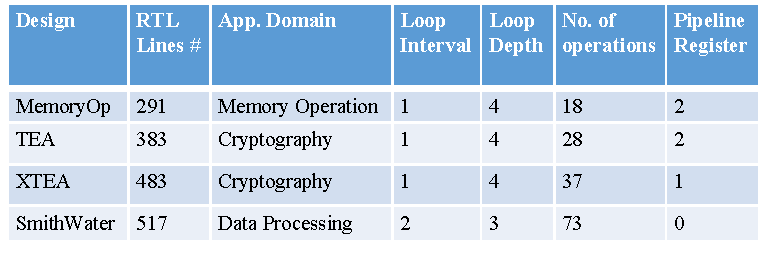
\includegraphics[width=5.5in]{fig-proposal/testing}
\end{center}
\caption{Behaviorally synthesized pipelined designs tested using our algorithm}
\label{fig:testing}
\end{figure}


We have successfully tested the pipeline reference model generated by our certified algorithm with the pipelined reference model generated by the previous algorithm. The test designs are non-trivial to pipeline with varied pipeline intervals and depths and require data forwarding and use of temporary shadow registers to remove data hazards. 

\section{Walk Through of Our Approach on an Industrial Strength Design}

To understand our approach, we can go over the steps of one particular industrial strength design.

\begin{figure}[H]
\begin{center}
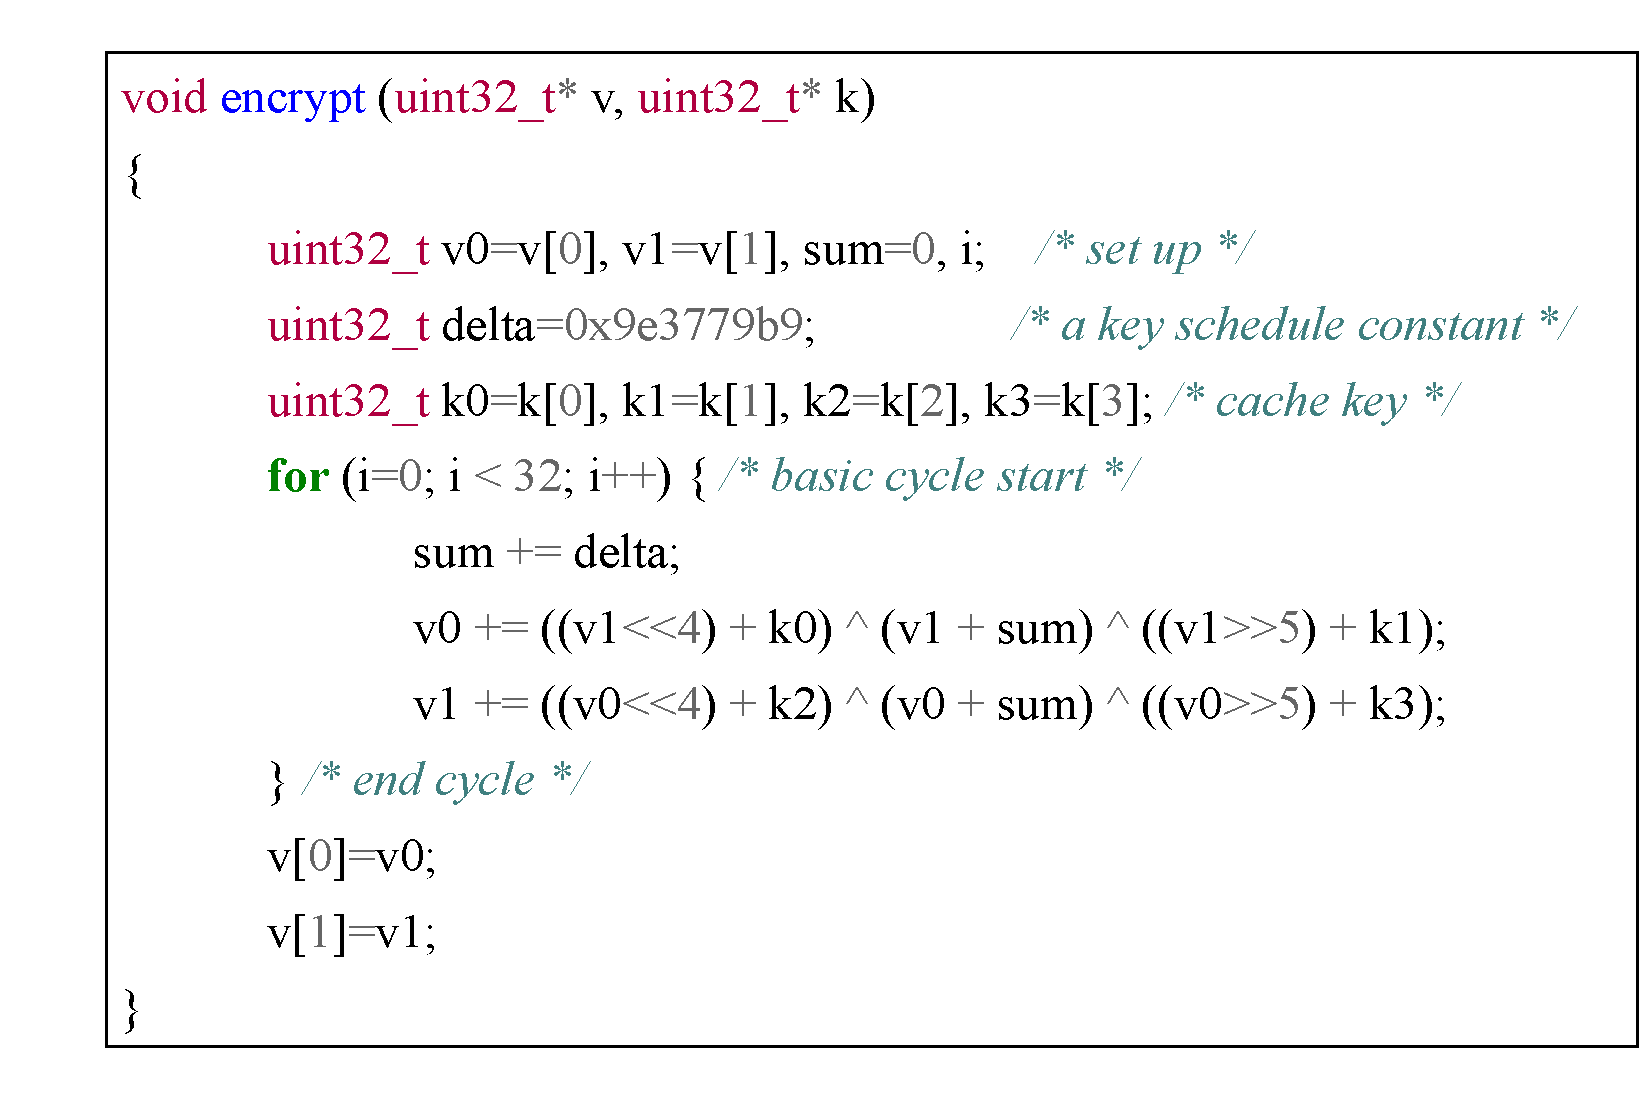
\includegraphics[width=5.5in]{fig-proposal/C-code-tea}
\end{center}
\caption{TEA: C code}
\label{fig:C-code-tea}
\end{figure}

Tiny Encryption Algorithm (TEA)~\cite{book-tea1} is a cryptography design. It is a block cipher notable for its simplicity of description and implementation with a few lines of code as shown in Figure~\ref{fig:C-code-tea}. TEA operates on two 32-bit unsigned integers (could be derived from a 64-bit data block) and uses a 128-bit key.  It has a simple key usage, mixing all of the key material in exactly the same way for each cycle. Different multiples of a magic constant are used to prevent simple attacks based on the symmetry of the rounds. The magic constant, 2654435769 or 9E3779B916 is chosen to be 232/$\phi$, where $\phi$ is the golden ratio''.  

The C code is converted to an Intermediate representation $IR$ and undergoes compiler transformations. If we only consider the loop CCDFG, ignoring the paraphernalia before and after this, we have a loop sequential CCDFG just before the loop pipelining transformtion needs to be applied as shown in Figure~\ref{fig:tea-seq-loop-ccdfg}. Now, we show how we apply our algorithm to derive a pipelined loop structure from this sequential CCDFG. 

Recall that the first step of the algorithm is to remove branches. Assuming that the loop exits in the (k + 1)st iteration, we separate $S_{loop}$ and $S_{preExit}$ as we explained earlier in Chapter 5. We now have a CCDFG as shown in Figure~\ref{fig:tea-algorithm-after-removing-branches}.

Next, we unroll the loop once to separate the first iteration from the rest. Recall that this step is important so that we can statically determine how to resolve the 
$\phi$-construct. The unrolled loop structure is shown in Figure~\ref{fig:tea-algorithm-two-iterations}.

Next, we resolve the $\phi$-construct and replace it with appropriate assignment statements as explained in $\phi$-removal step in Chapter 5. Note that the
first iteration of the loop has the previous basic block as $Entry$ so $\phi$-construct resolution is different than those in other iterations where previous basic block is $Z$. The CCDFG after this step is as shown in Figure~\ref{fig:tea-after-phi-removal}.

\begin{figure}[H]
\begin{center}
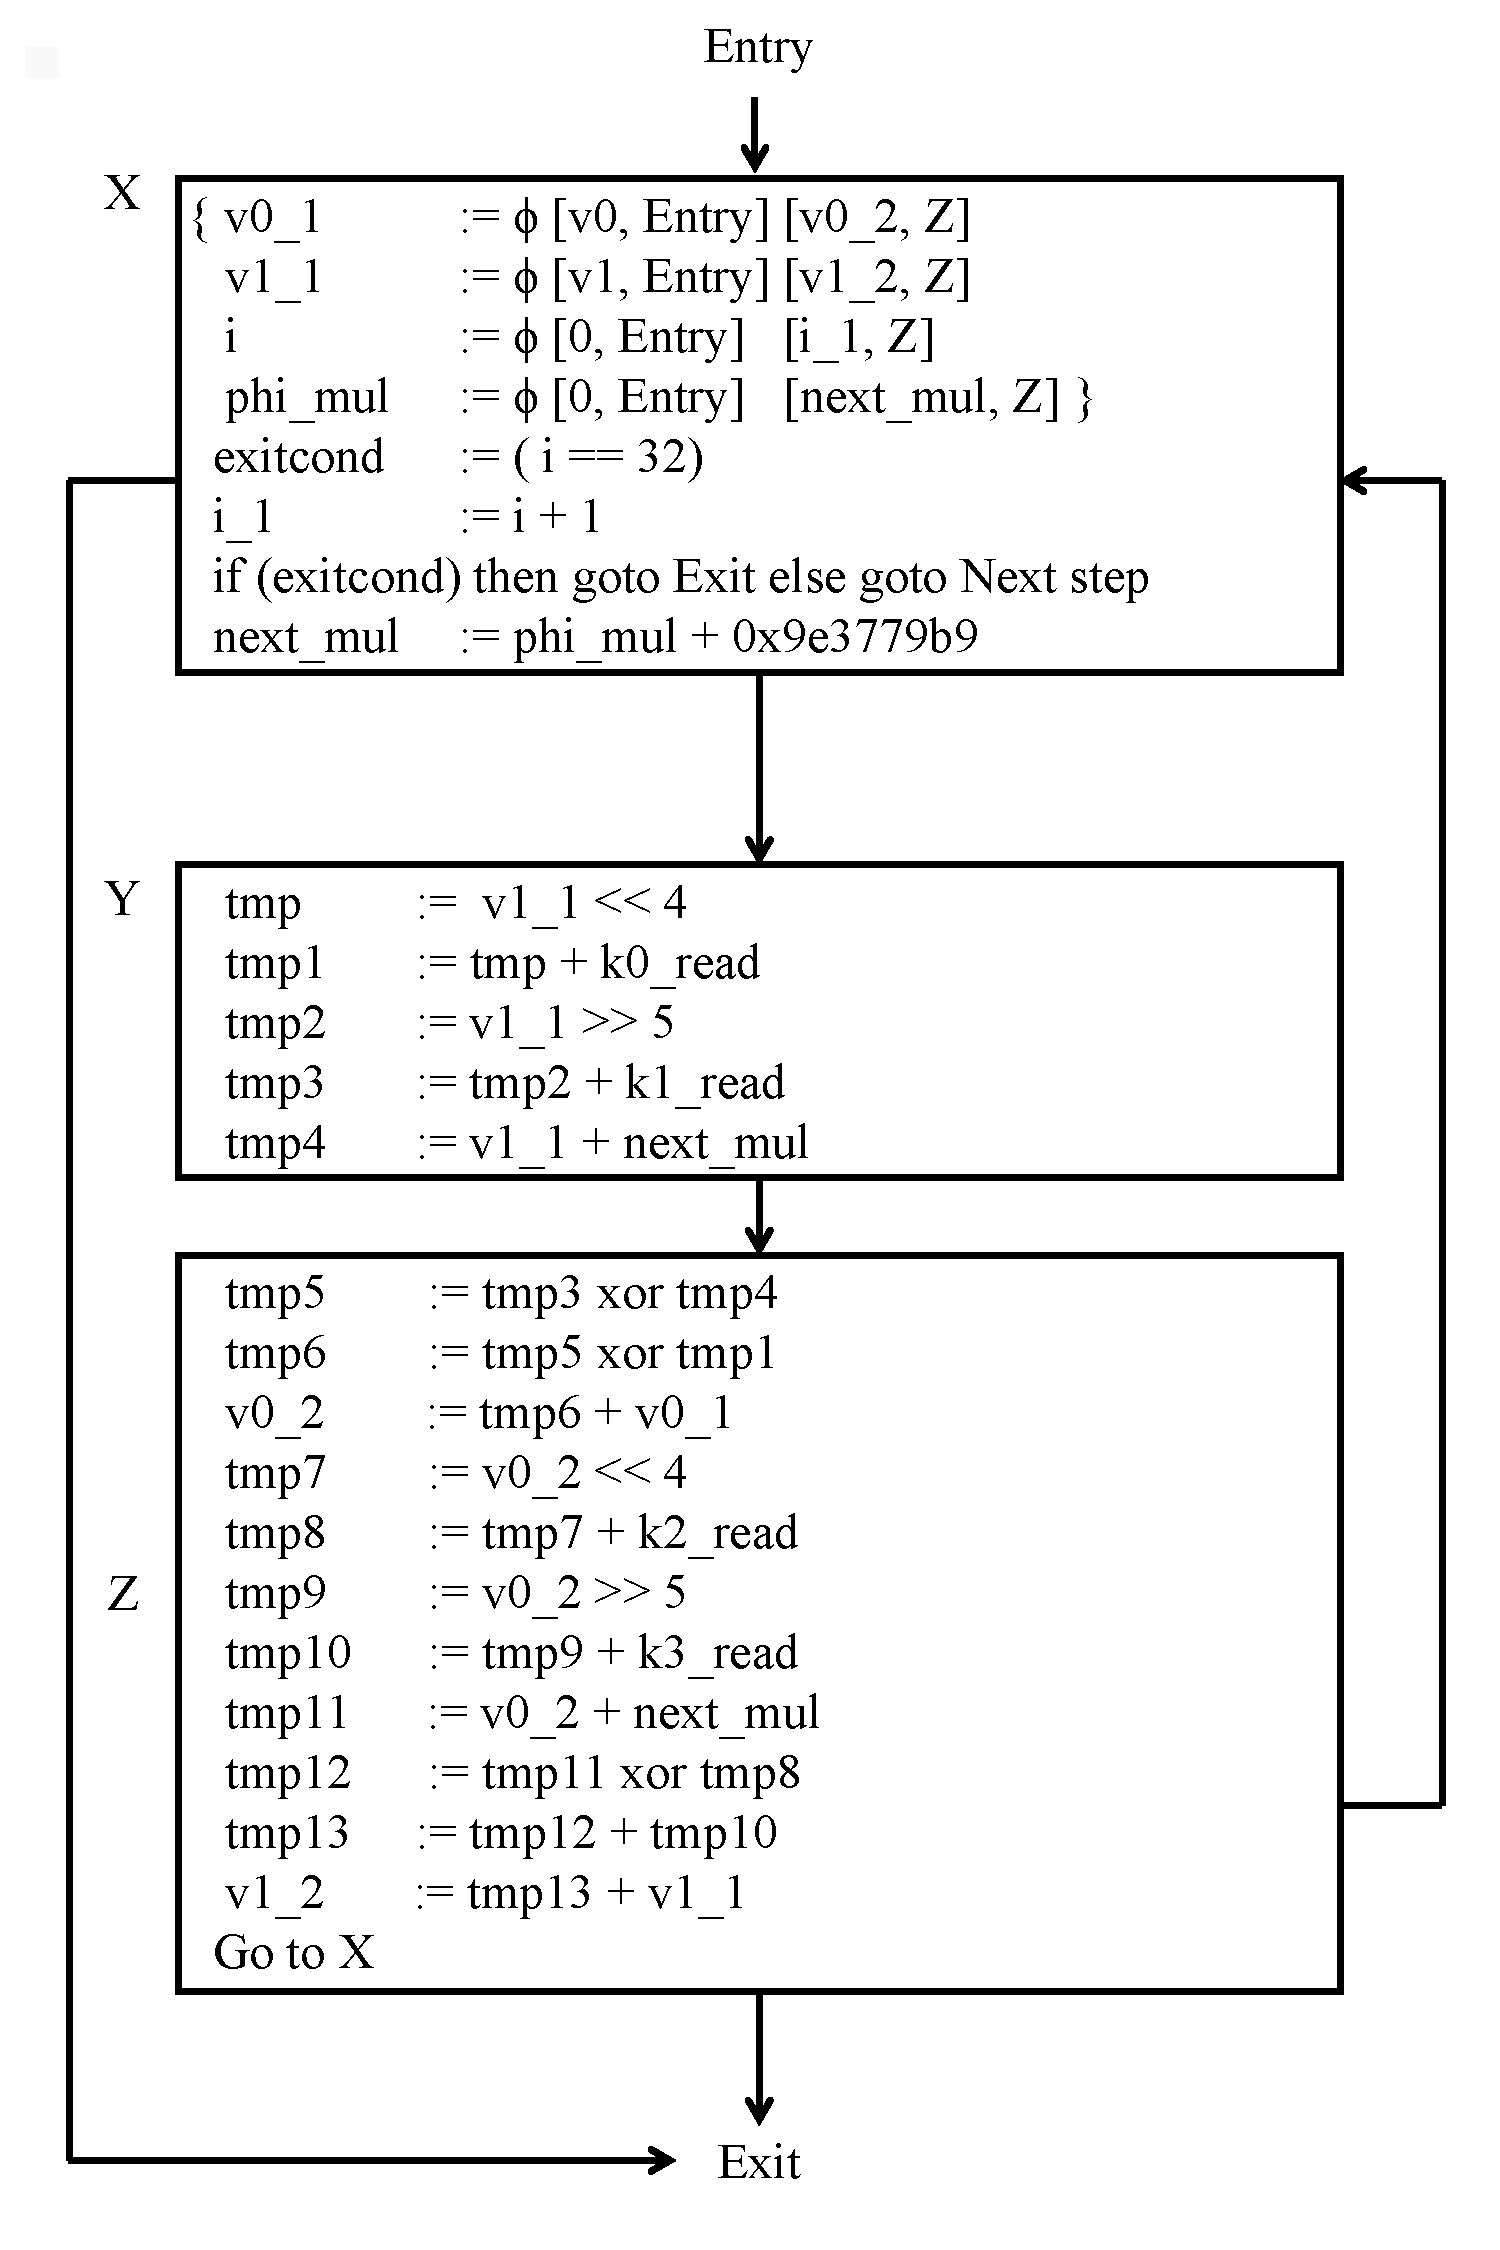
\includegraphics[width=4.75in]{fig-proposal/tea-seq-ccdfg}
\caption{TEA: Sequential loop CCDFG}
\label{fig:tea-seq-loop-ccdfg}
\end{center}
\end{figure}

\begin{figure}[H]
\begin{center}
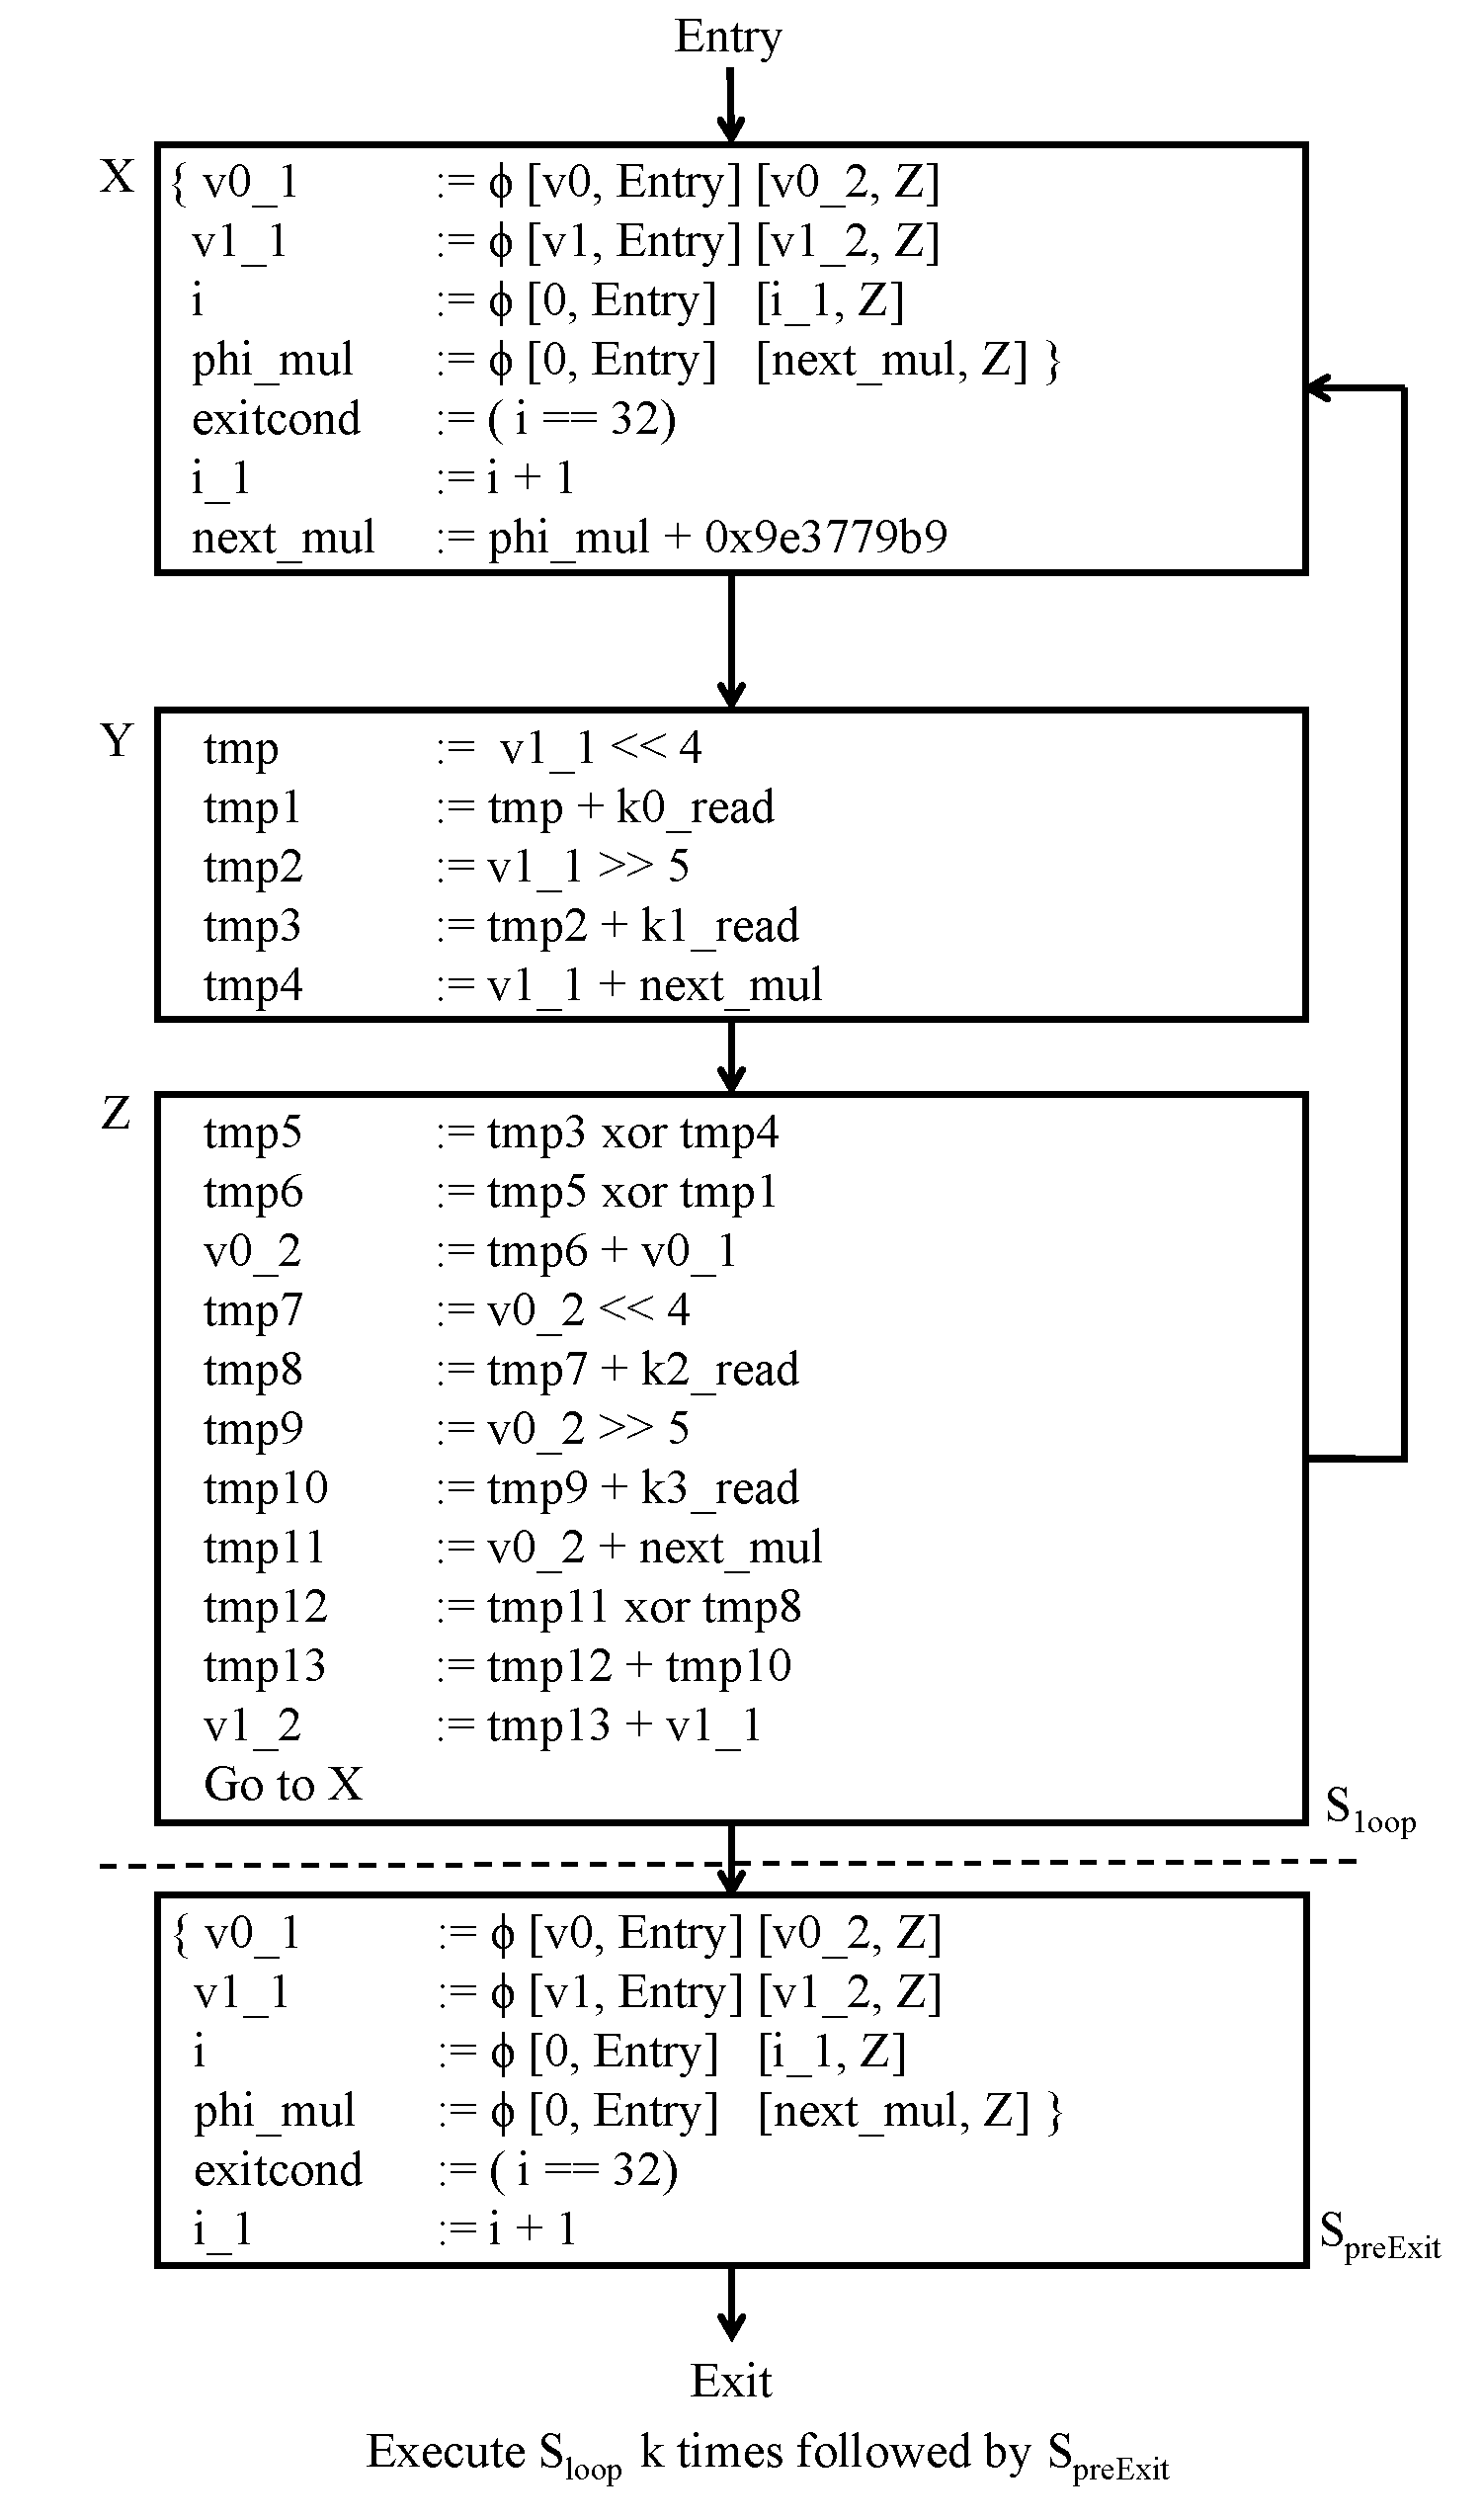
\includegraphics[height=8in]{fig-proposal/tea-algorithm-after-removing-branches}
\caption{TEA: After removing branches}
\label{fig:tea-algorithm-after-removing-branches}
\end{center}
\end{figure}

\begin{figure}[H]
\begin{center}
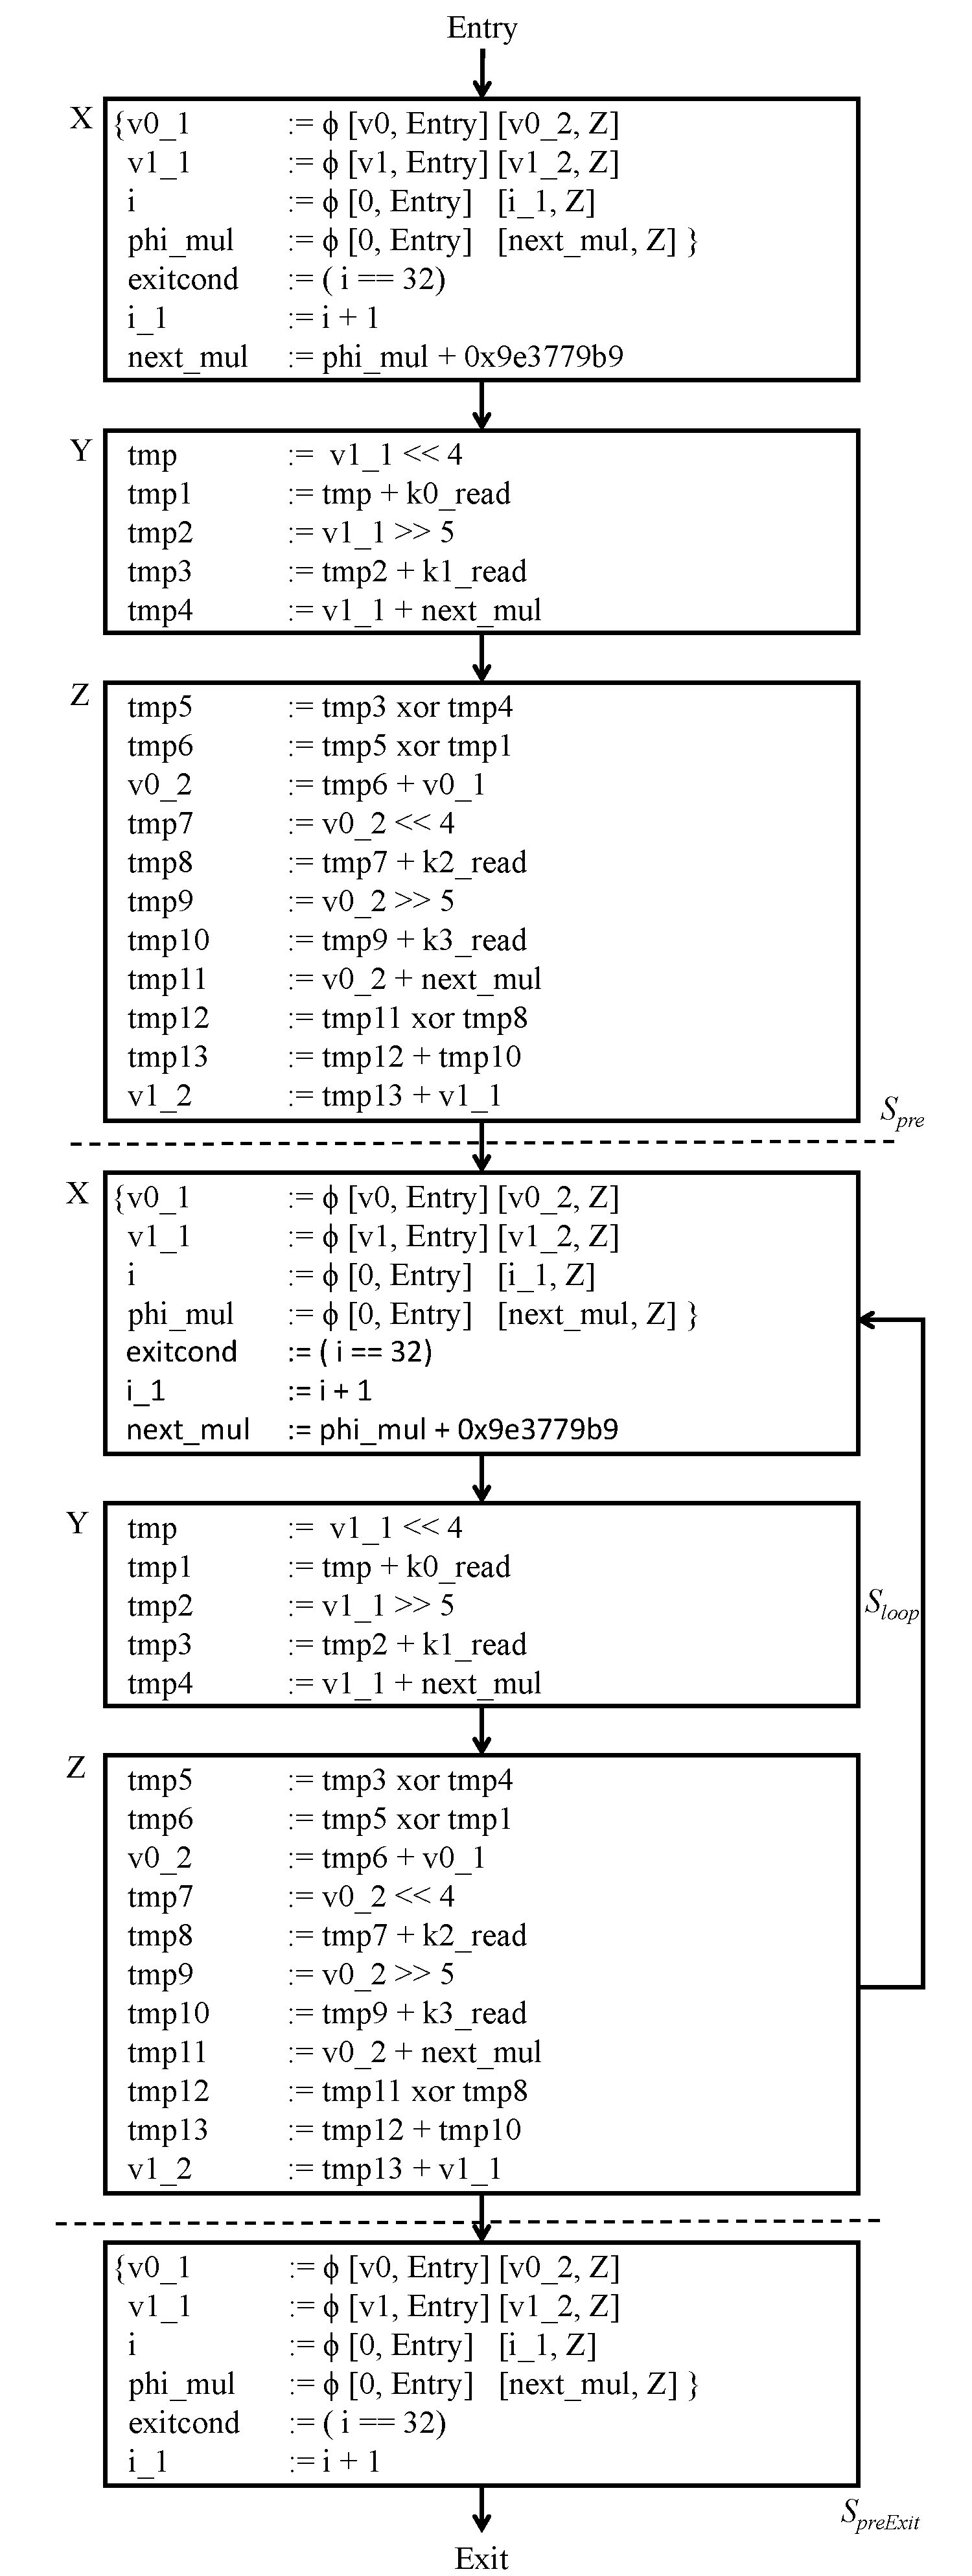
\includegraphics[height=8in]{fig-proposal/tea-after-two-iterations}
\caption{TEA: After unrolling loop once}
\label{fig:tea-algorithm-two-iterations}
\end{center}
\end{figure}


\begin{figure}[H]
\begin{center}
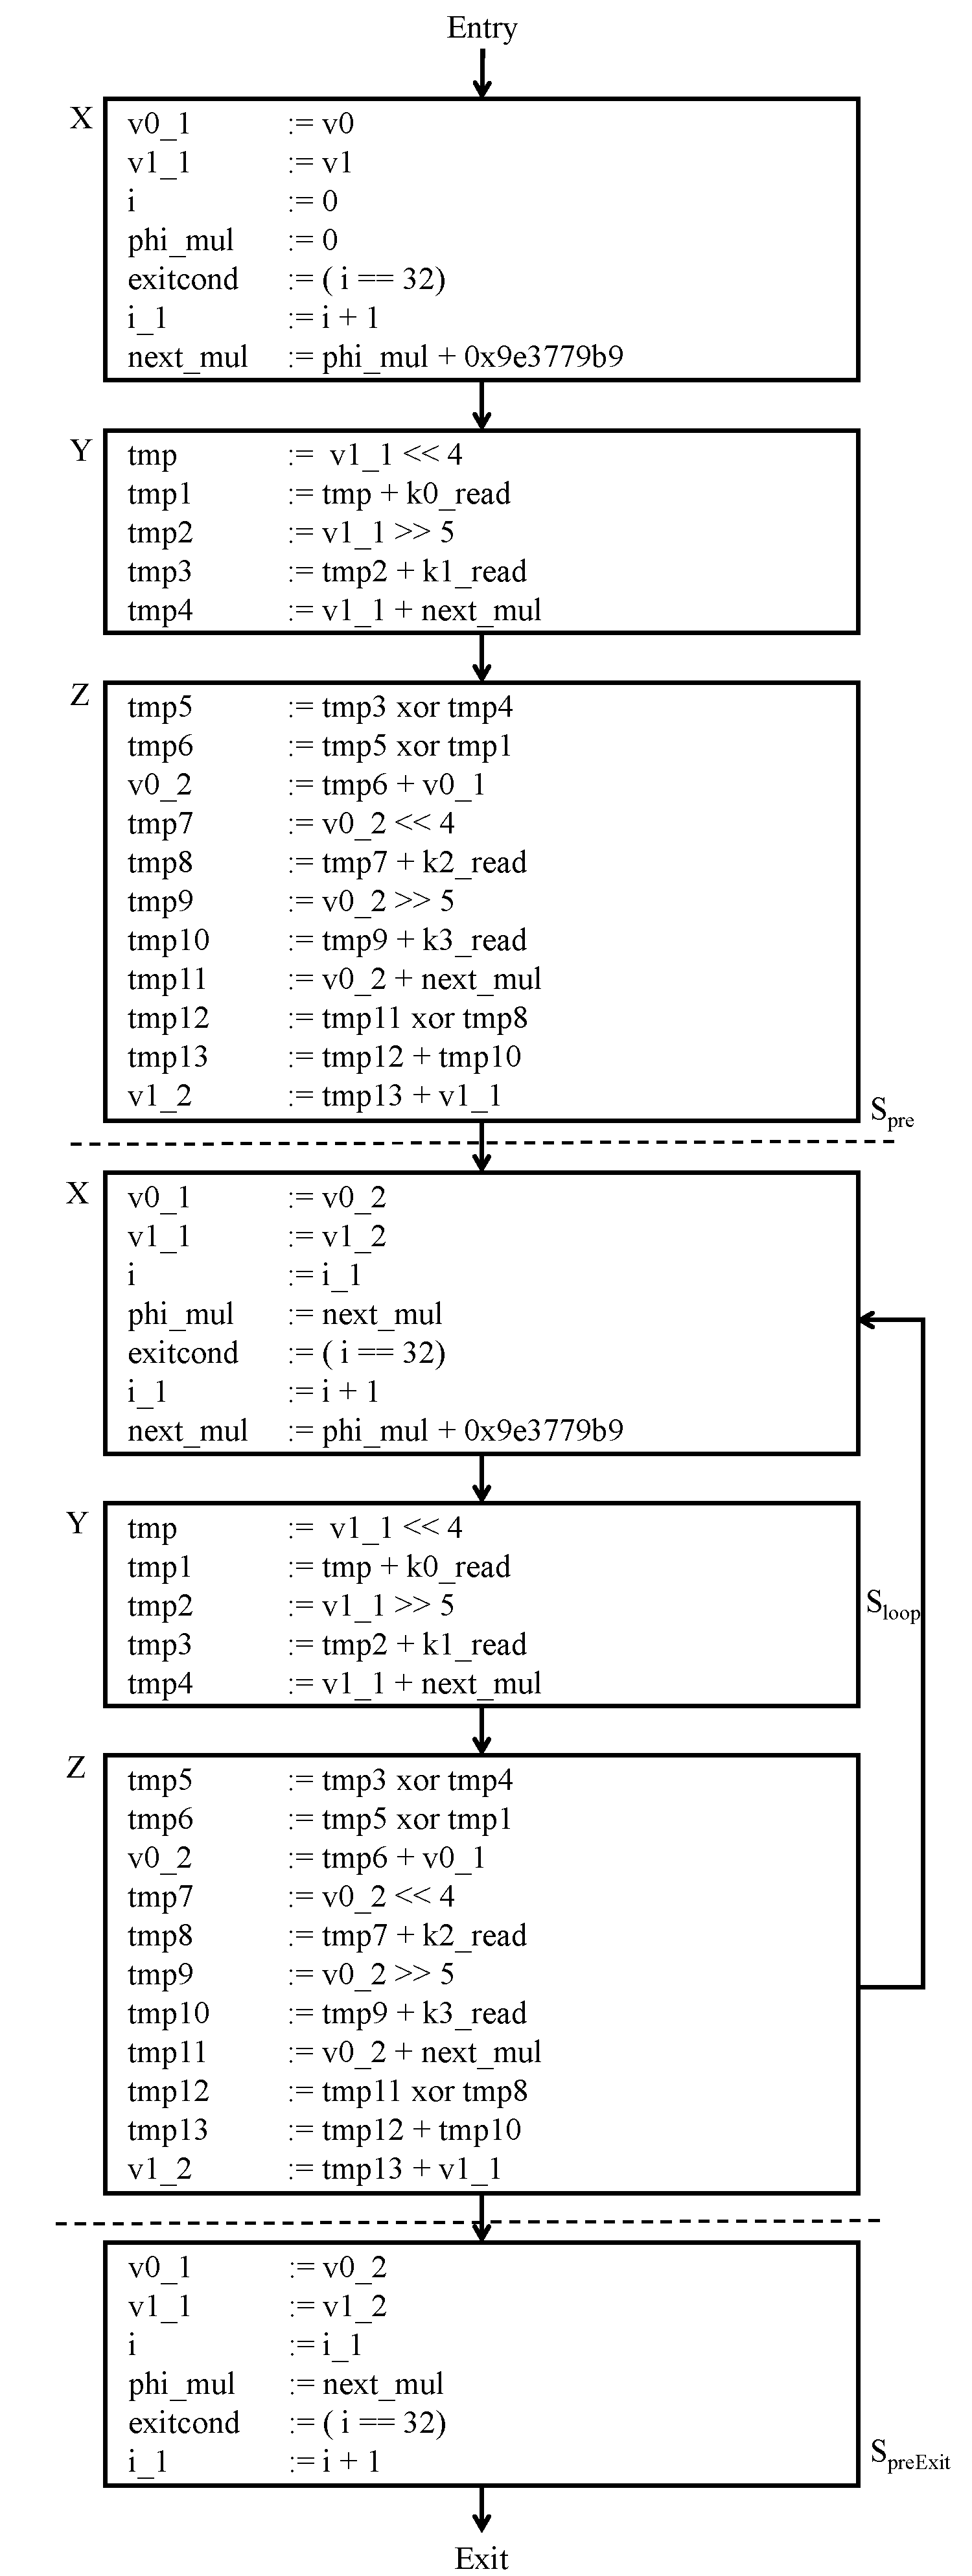
\includegraphics[height=8in]{fig-proposal/tea-after-phi-removal}
\caption{TEA: After $\phi$-removal}
\label{fig:tea-after-phi-removal}
\end{center}
\end{figure}

Now, we have to prepare this CCDFG so that iterations can be overlapped. So, we need to remove the data hazards. We first identify the variables/microsteps which 
cause Write After Read (WAR) hazards. We note that values of v0\_1 and v1\_1 are read in $X$ and written in $Z$ of $S_{loop}$. If we overlap the iterations, then $X$ of second iteration will read the outdated values of these variables before they have had a chance to be updated by the $Z$ of the first iteration, thus causing data hazards. 

To overcome this, recall that we have data propagation step in Chapter 5 as next step of our algorithm. We implement the first step for $v0\_1 := v0\_2$ 
and move it to the beginning of the X block in $S_{loop}$ and $S_{preExit}$ as shown in Figure~\ref{fig:tea-after-data-propagation1}. Since, we are already at the beginning of $S_{loop}$ here, nothing needs to be done. Recall, this step may need multiple applictions of interchange primitive. 

In the second step, we add this microstep to $Z$ of $S_{pre}$ and $Z$ of $S_{loop}$ and remove this mstep from $X$ of $S_{loop}$ and $X$ of $S_{preExit}$ as shown in Figure~\ref{fig:tea-after-data-propagation2}. The motivation is to move the microstep to the previous iteration such that the value of any variable is overwritten only when the previous value has already been correctly read. The justification of this step is as explained in Chapter 6 using smart restructing of CCDFG to ease the complexity and application of multiple interchange primitives. 

We apply both the steps of data propagation primitive for the second mstep as well, as shown $v1\_1 := v1\_2$ in Figures~\ref{fig:tea-after-data-propagation3} and~\ref{fig:tea-after-data-propagation4}.

\begin{figure}[H]
\begin{center}
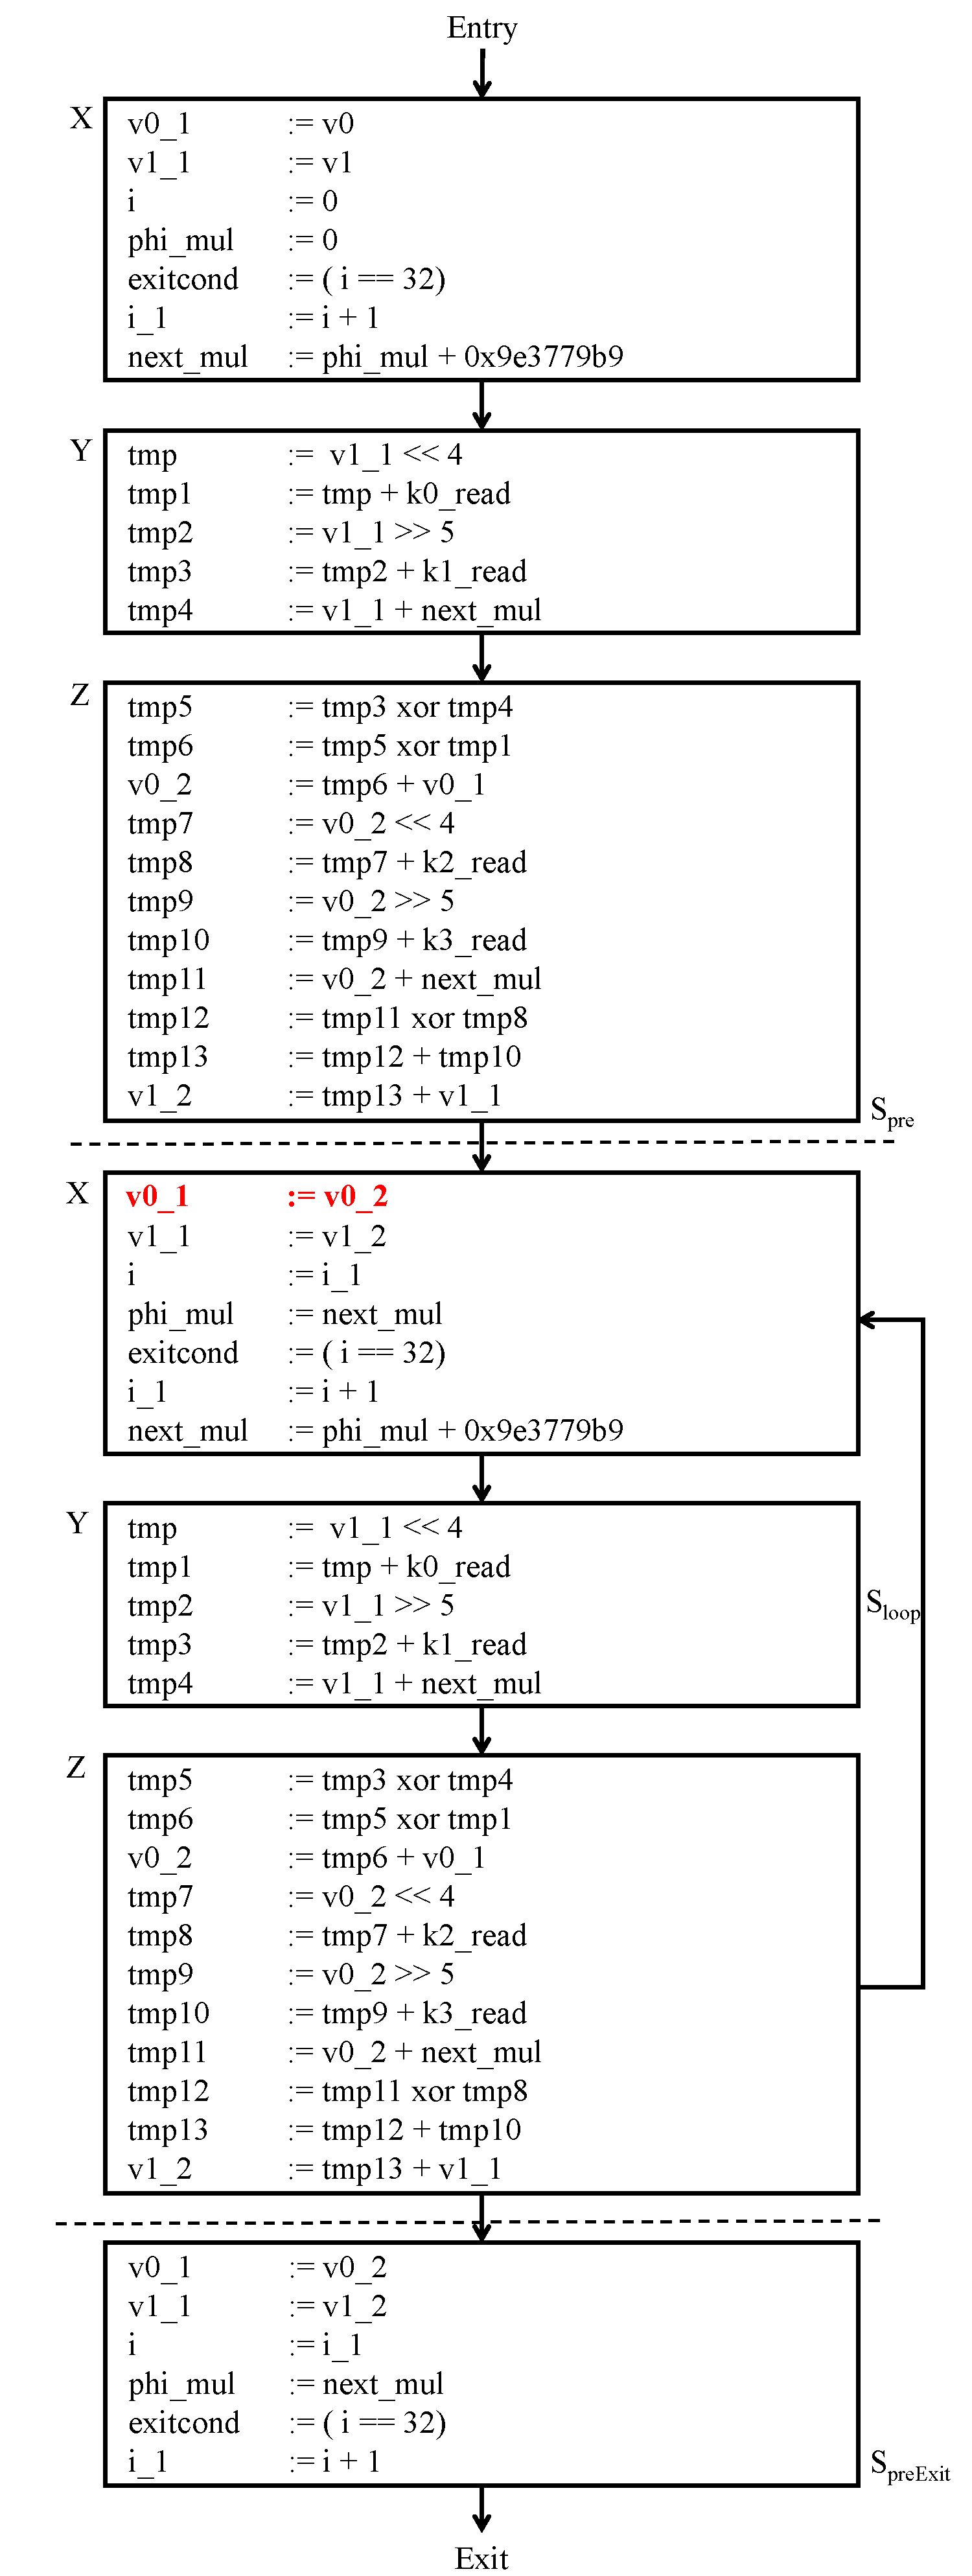
\includegraphics[height=8in]{fig-proposal/tea-after-data-propagation1}
\caption{TEA: After data propagation first step for $v0\_1 := v0\_2$}
\label{fig:tea-after-data-propagation1}
\end{center}
\end{figure}

\begin{figure}[H]
\begin{center}
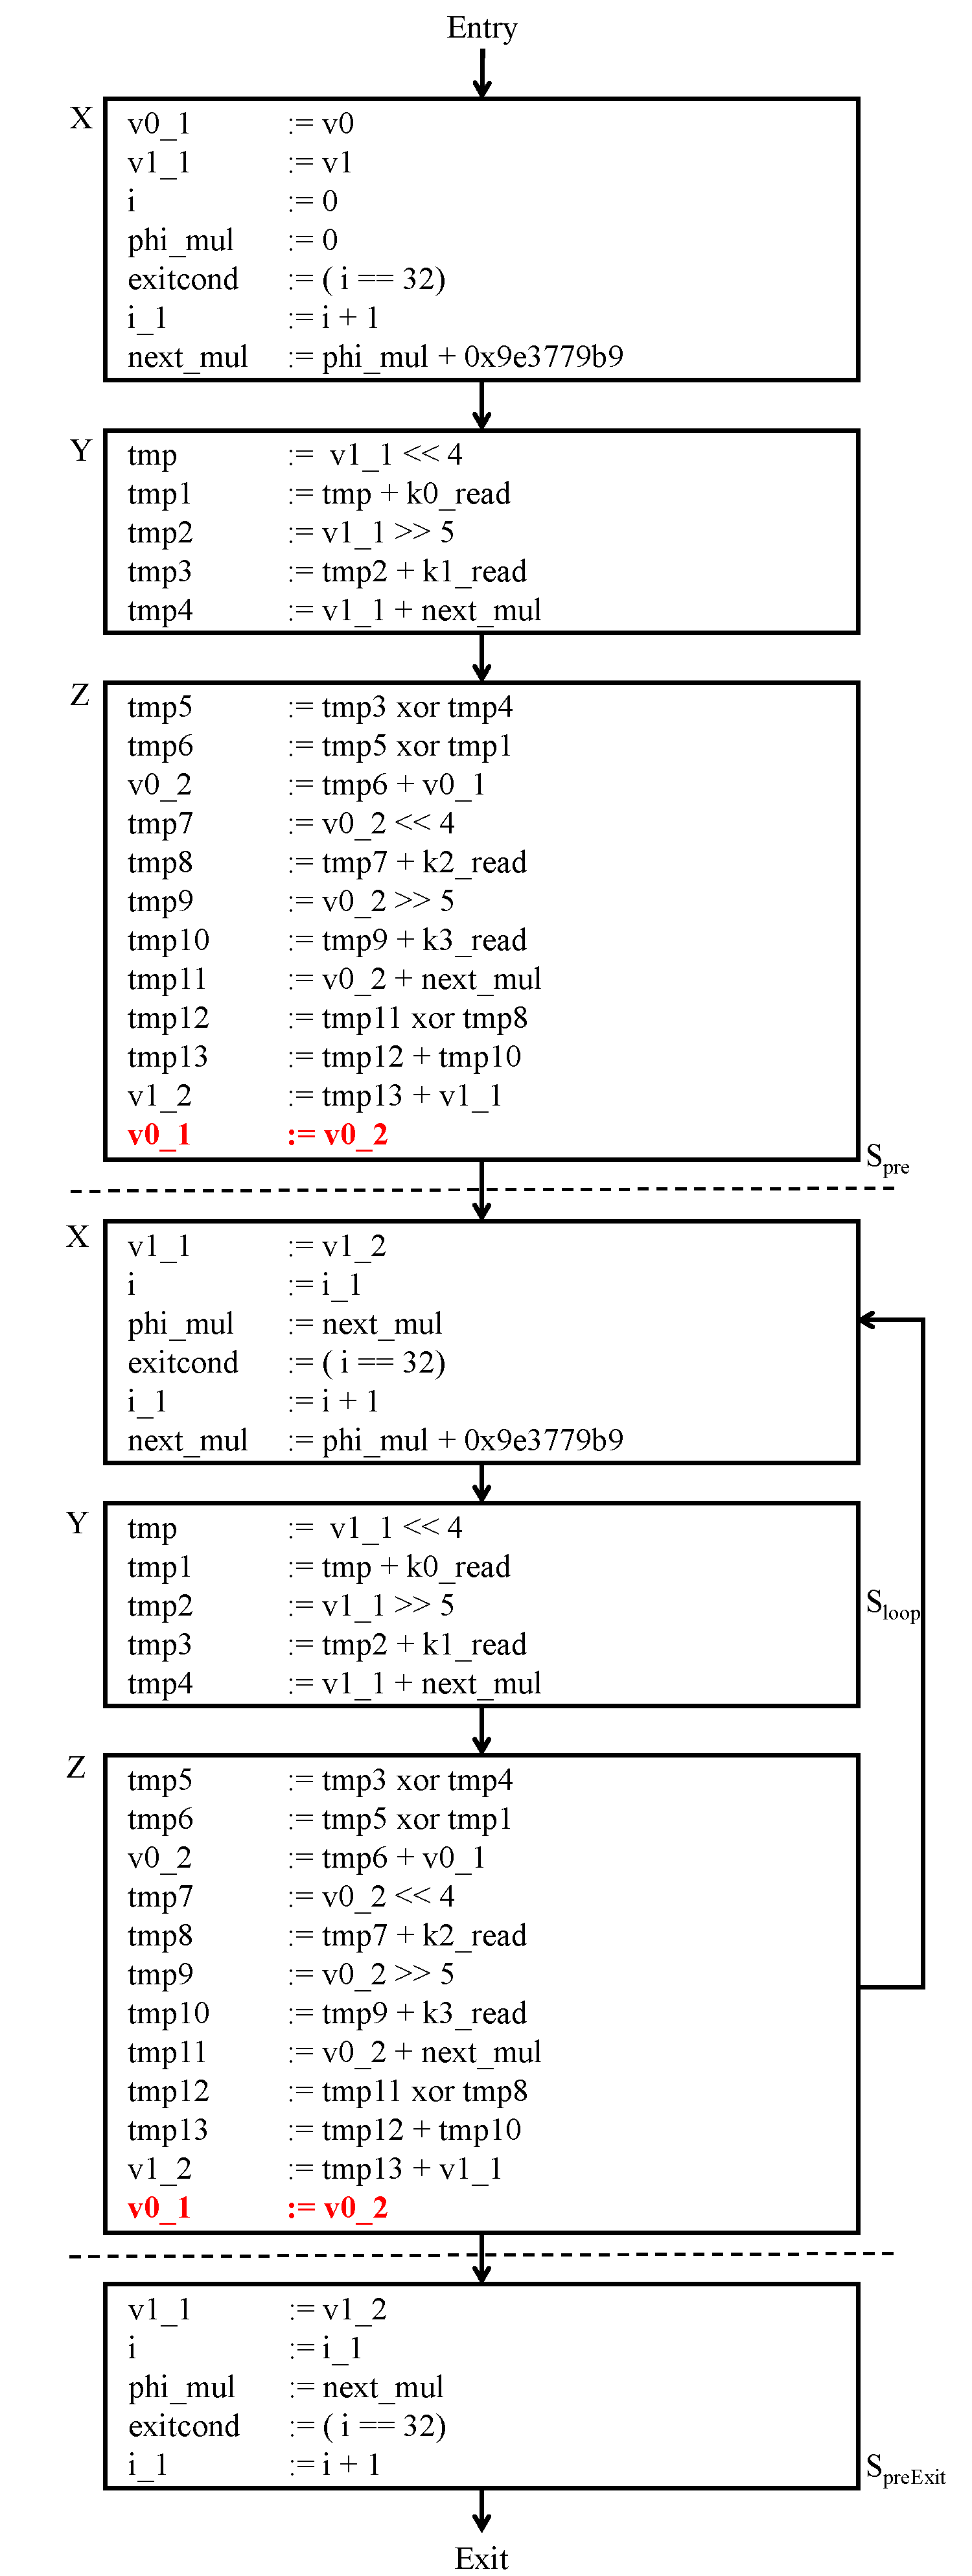
\includegraphics[height=8in]{fig-proposal/tea-after-data-propagation2}
\caption{TEA: After data propagation second step for $v0\_1 := v0\_2$}
\label{fig:tea-after-data-propagation2}
\end{center}
\end{figure}

\begin{figure}[H]
\begin{center}
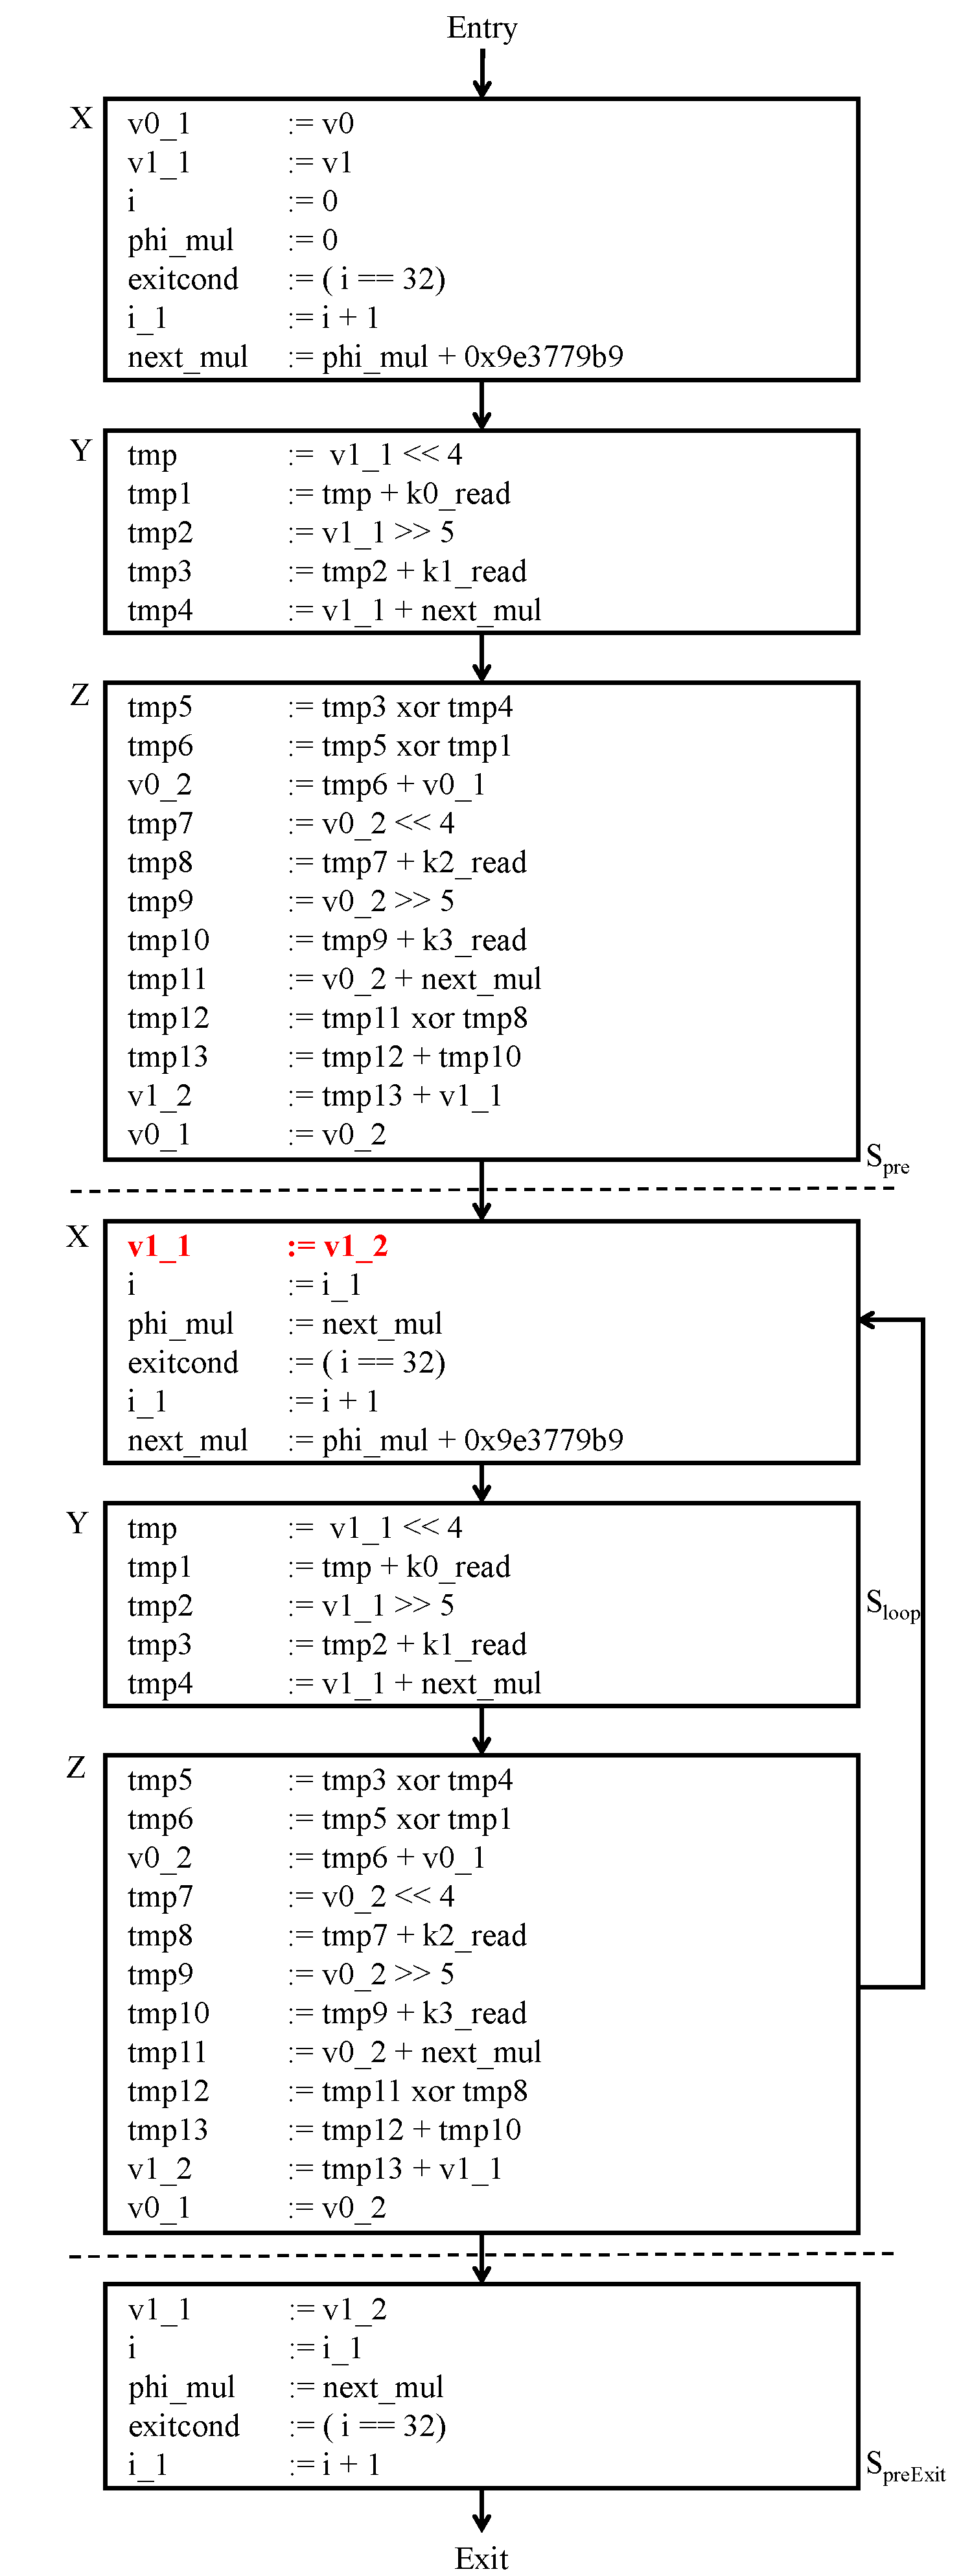
\includegraphics[height=8in]{fig-proposal/tea-after-data-propagation3}
\caption{TEA: After data propagation first step for $v1\_1 := v1\_2$}
\label{fig:tea-after-data-propagation3}
\end{center}
\end{figure}

\begin{figure}[H]
\begin{center}
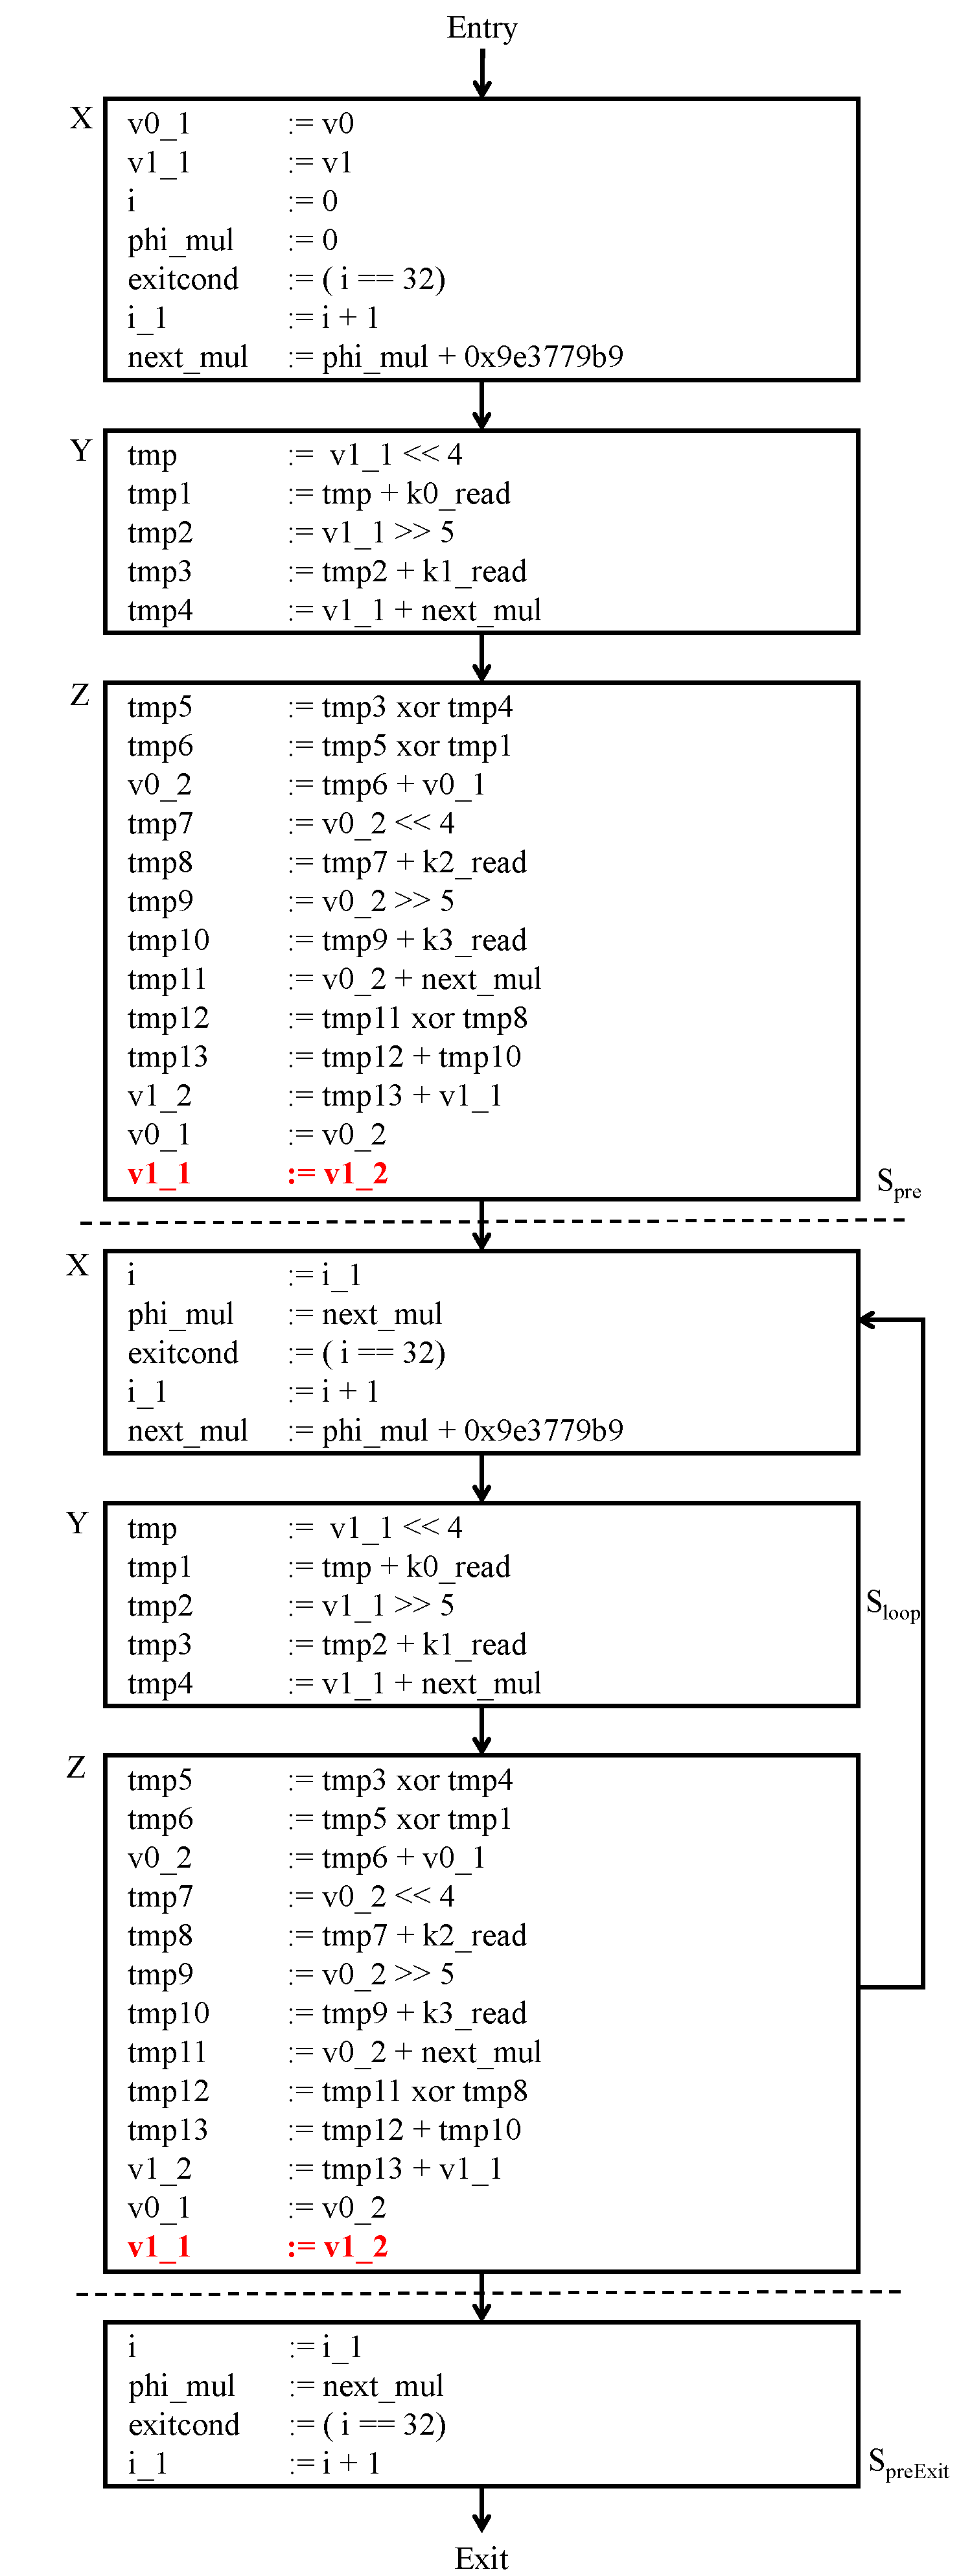
\includegraphics[height=8in]{fig-proposal/tea-after-data-propagation4}
\caption{TEA: After data propagation second step for $v1\_1 := v1\_2$}
\label{fig:tea-after-data-propagation4}
\end{center}
\end{figure}

After we have removed the potential WAR hazards which can stall the pipeline, we need to remove the RAW hazards as well.
We check the variables which can cause data hazards by measuring the read and write distance between variables 
and compare it to pipeline interval. For example, in Figure~\ref{fig:tea-after-data-propagation4}, we write $next\_mul$ 
in $X$ while we read $next\_mul$ in both $Y$ and $Z$. 
If we overlap the iterations as it is, then the $X$ of second iteration occurs before $Z$ of first iteration and we overwrite the value in 
$X$ before $Z$ has a chance to read it. Note that we know this as our algorithm calculates the longest read and write distance of every variable 
in an iteration. Here the distance for $next\_mul$ is 2 scheduling steps, while the pipeline interval is 1. So, we know that this
variable will cause a hazard when we pipeline. For all other variables, the distance is either 1 or 0 which is less than the pipeline interval so we know that they are
safe. 

We store the value of the variable in temporary variables called shadow registers, here we store the value in next\_reg, for second scheduling
step, we store in next\_reg2 and we read from these shadow registers so that the original value is unaffected and can be read as required. The new CCDFG with 
temporary variables is shown in Figure~\ref{fig:tea-after-shadow-register}.

Now, we can overlap the iterations as shown in Figure~\ref{fig:tea-after-superstep-construction}. We call this step - superstep construction. 

Now, we need to add the branches back which is the final step of our algorithm. We first interchange the $S\_{preExit}$ with $P\_{post}$. Since we have already removed the potential data hazards, we know that we can apply interchange primitives to achieve this step as shown in Figure ~\ref{fig:tea-after-interchange-post-exit}. Then, we apply the branch primitive and put the branch back to get the final pipelined structure as shown in Figure~\ref{fig:tea-after-adding-branches}.
 

\begin{figure}[H]
\begin{center}
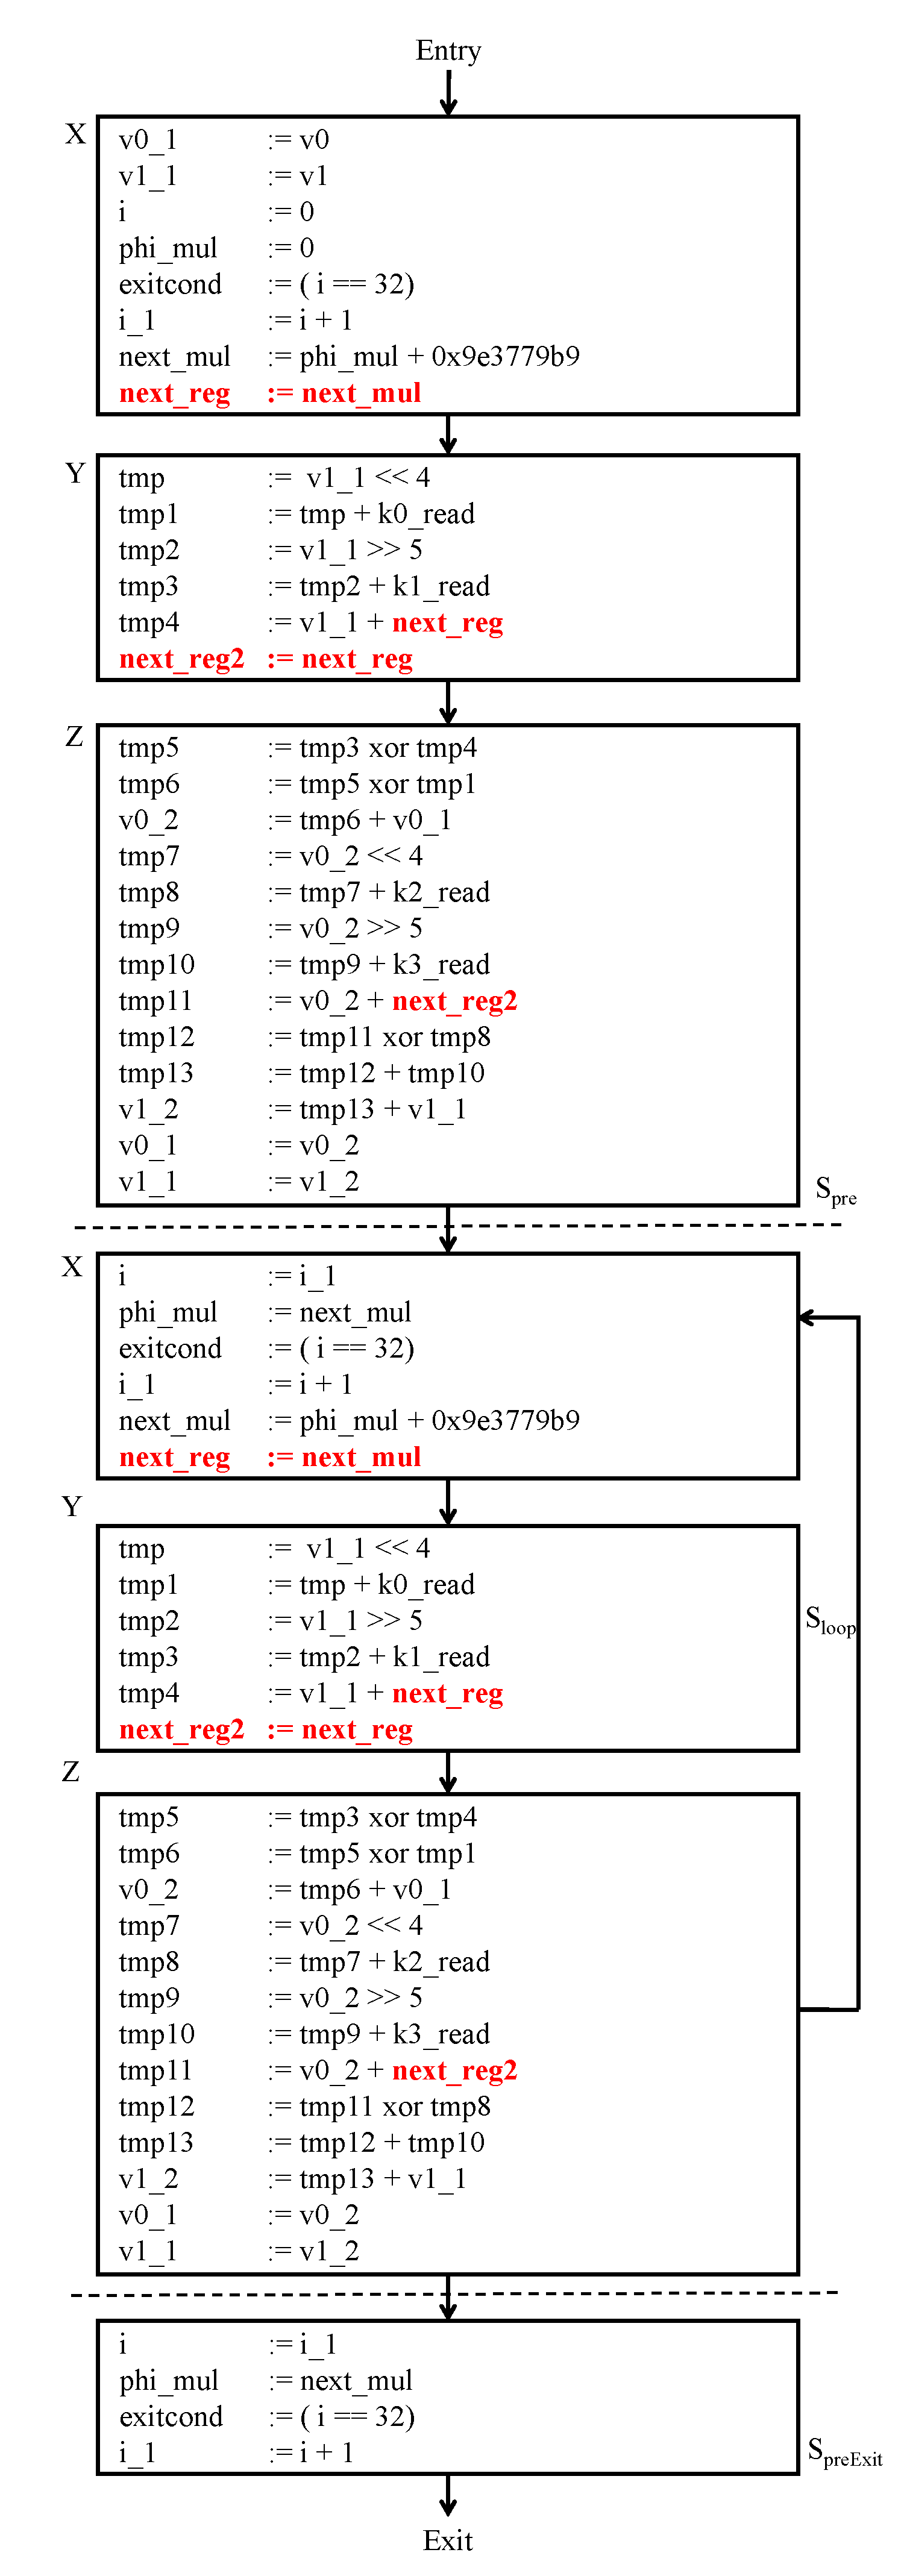
\includegraphics[height=8in]{fig-proposal/tea-after-shadow-reg}
\caption{TEA: After adding shadow registers}
\label{fig:tea-after-shadow-register}
\end{center}
\end{figure}



\begin{figure}[H]
\begin{center}
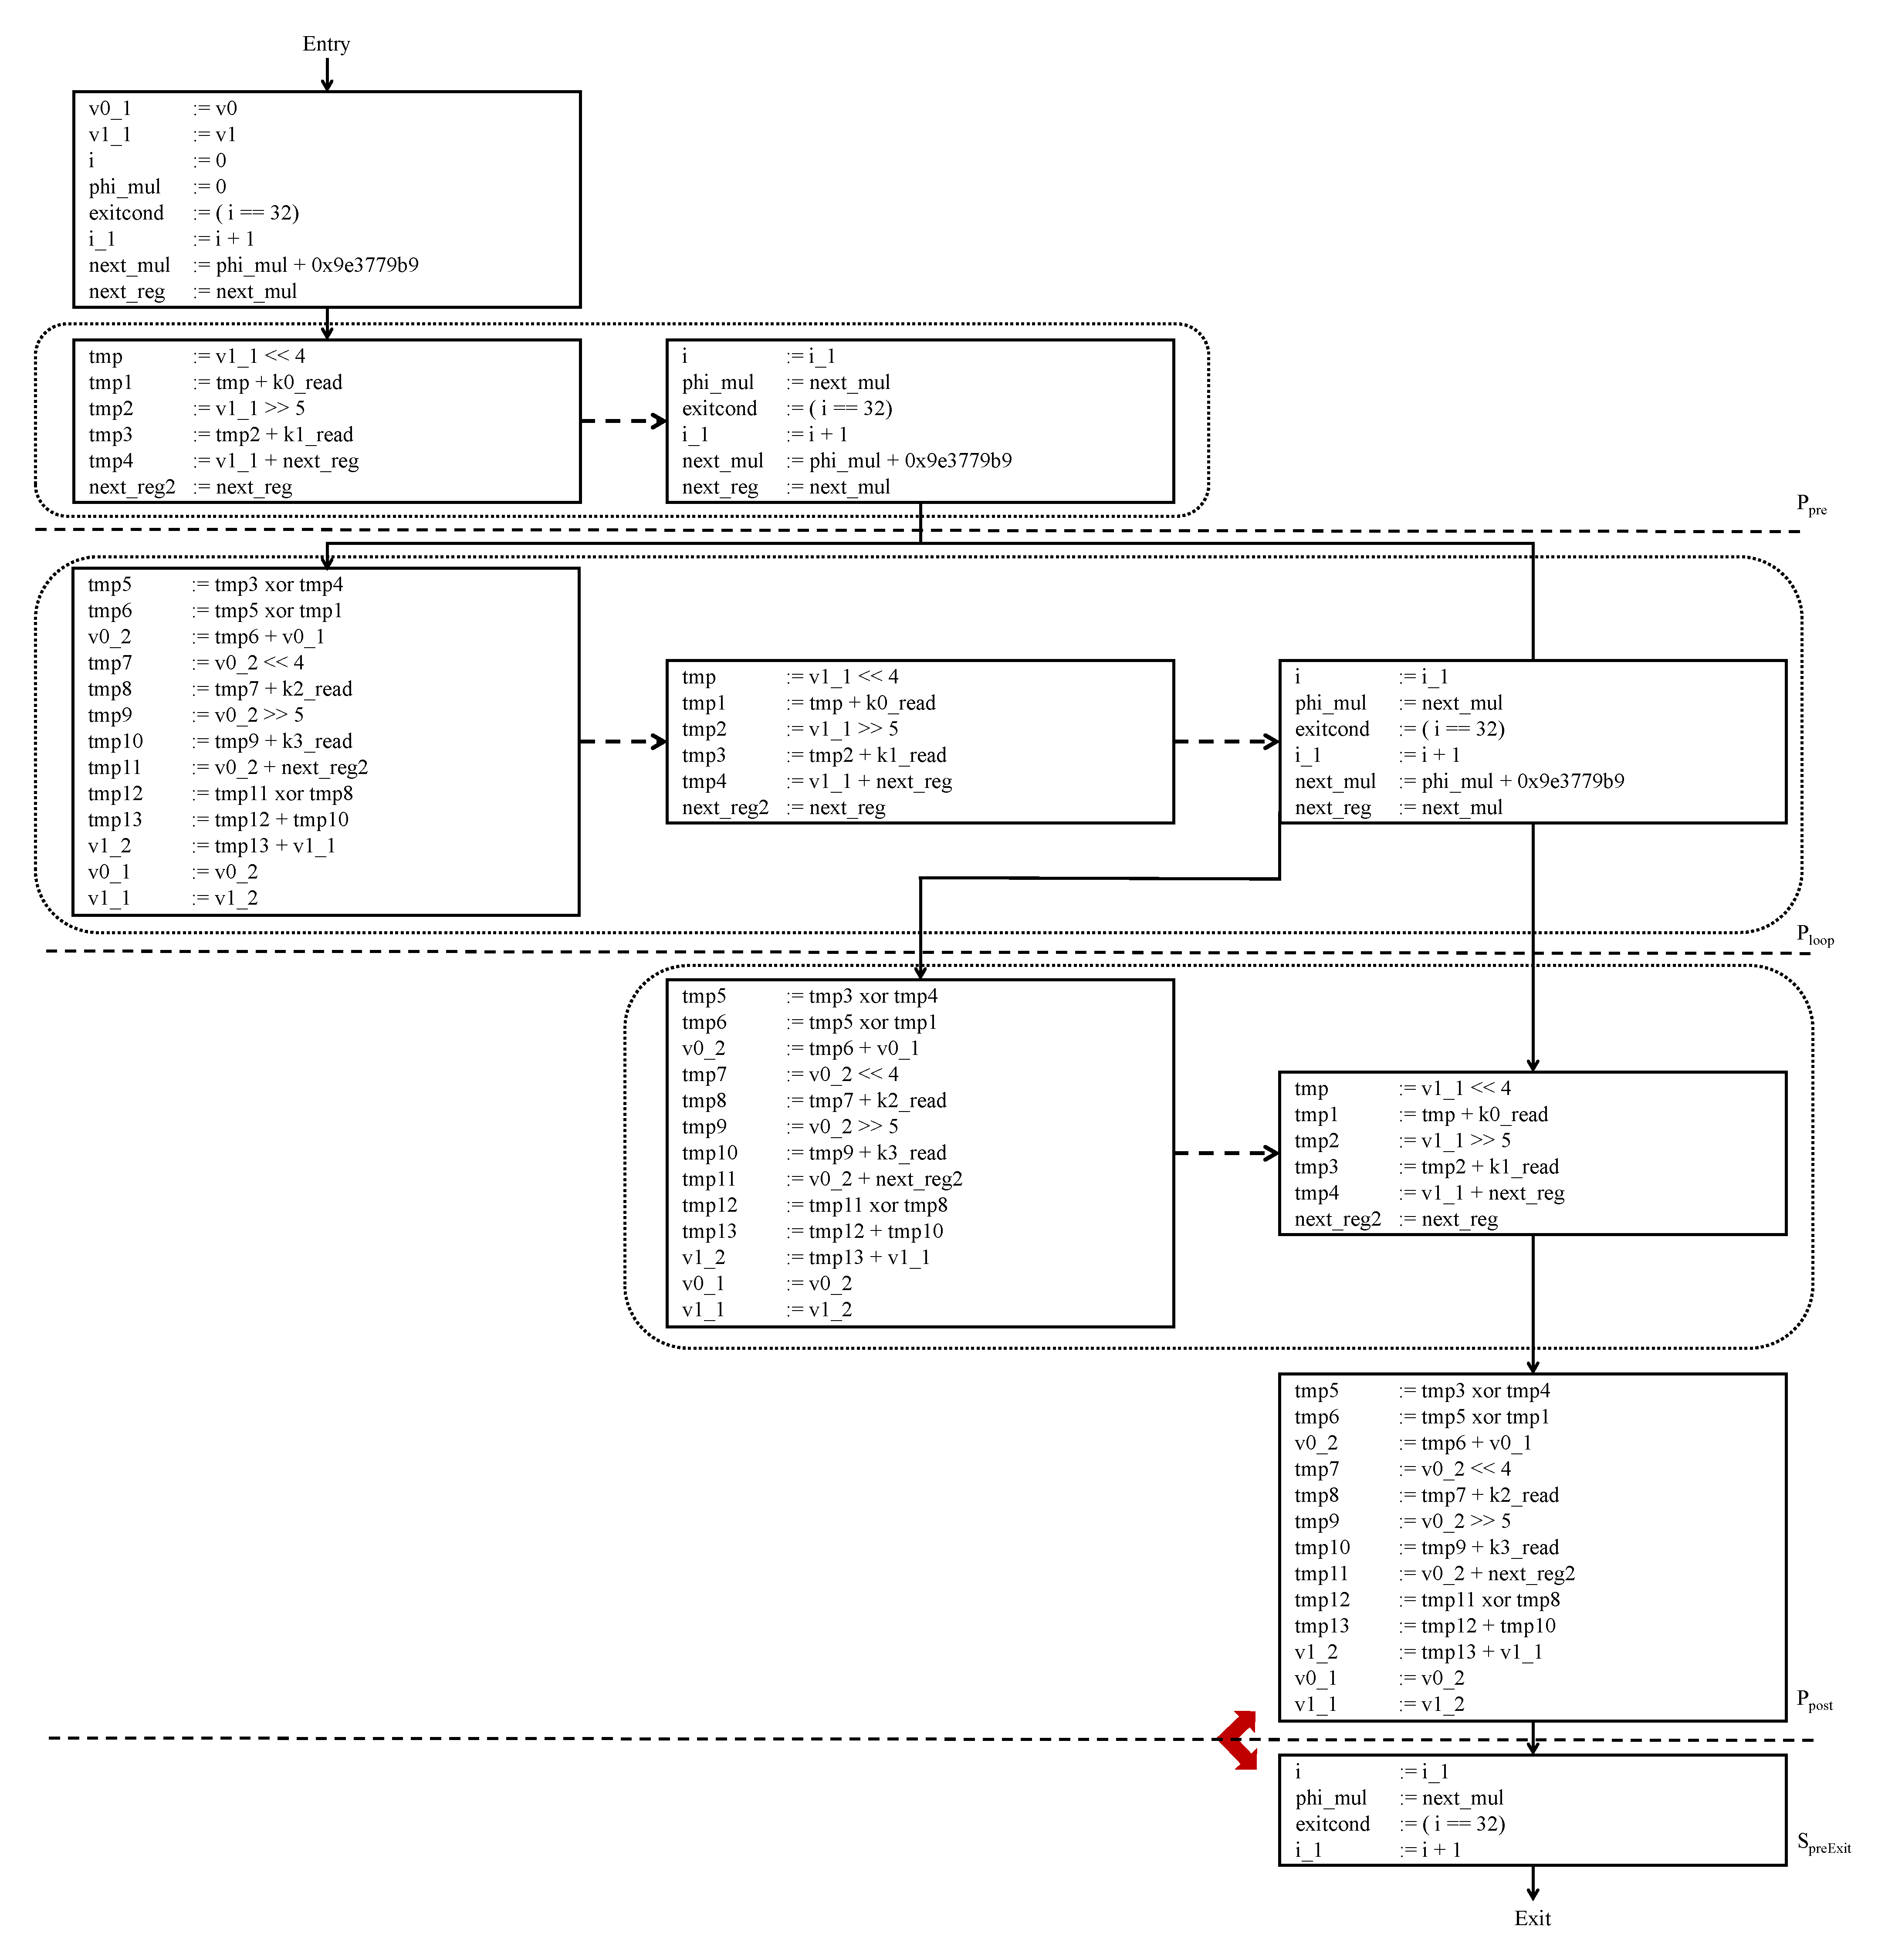
\includegraphics[width=5.5in]{fig-proposal/tea-after-superstep-construction}
\caption{TEA: After superstep construction}
\label{fig:tea-after-superstep-construction}
\end{center}
\end{figure}

\begin{figure}[H]
\begin{center}
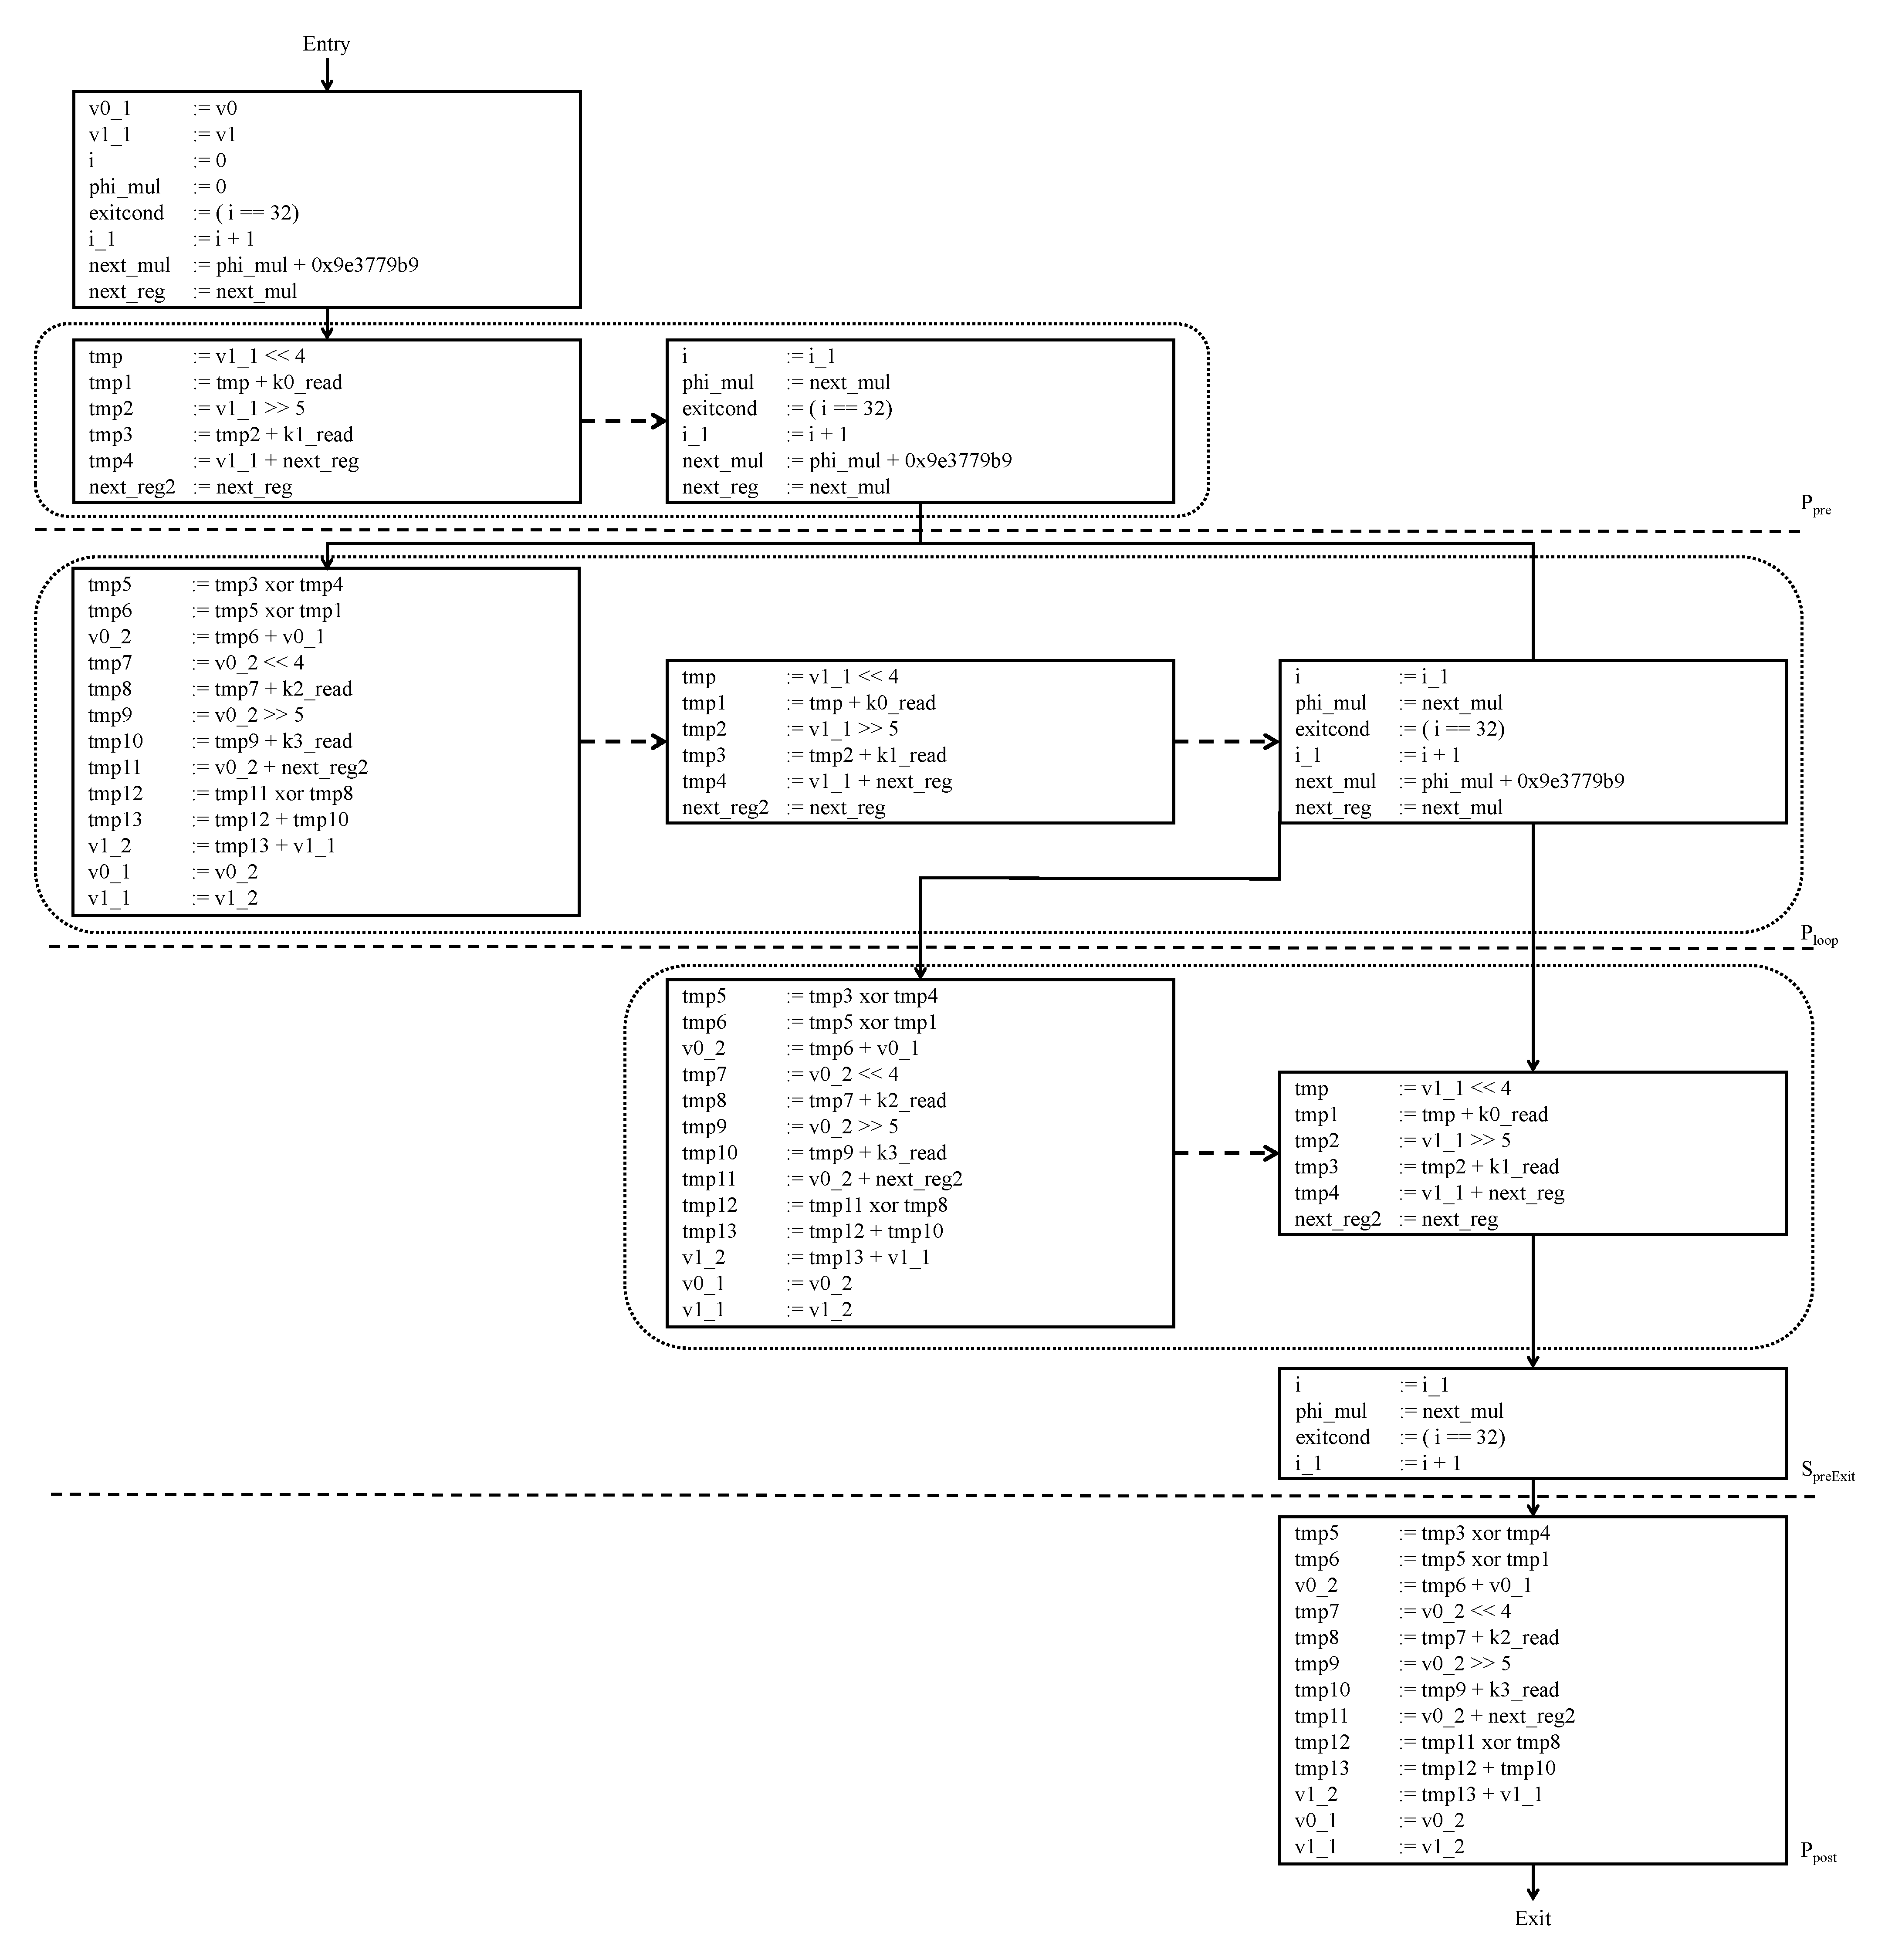
\includegraphics[width=5.5in]{fig-proposal/tea-after-interchange-pre-post}
\caption{TEA: After interchanging post with pre-exit}
\label{fig:tea-after-interchange-post-exit}
\end{center}
\end{figure}

\clearpage
\begin{sidewaysfigure}[t!]
\begin{center}
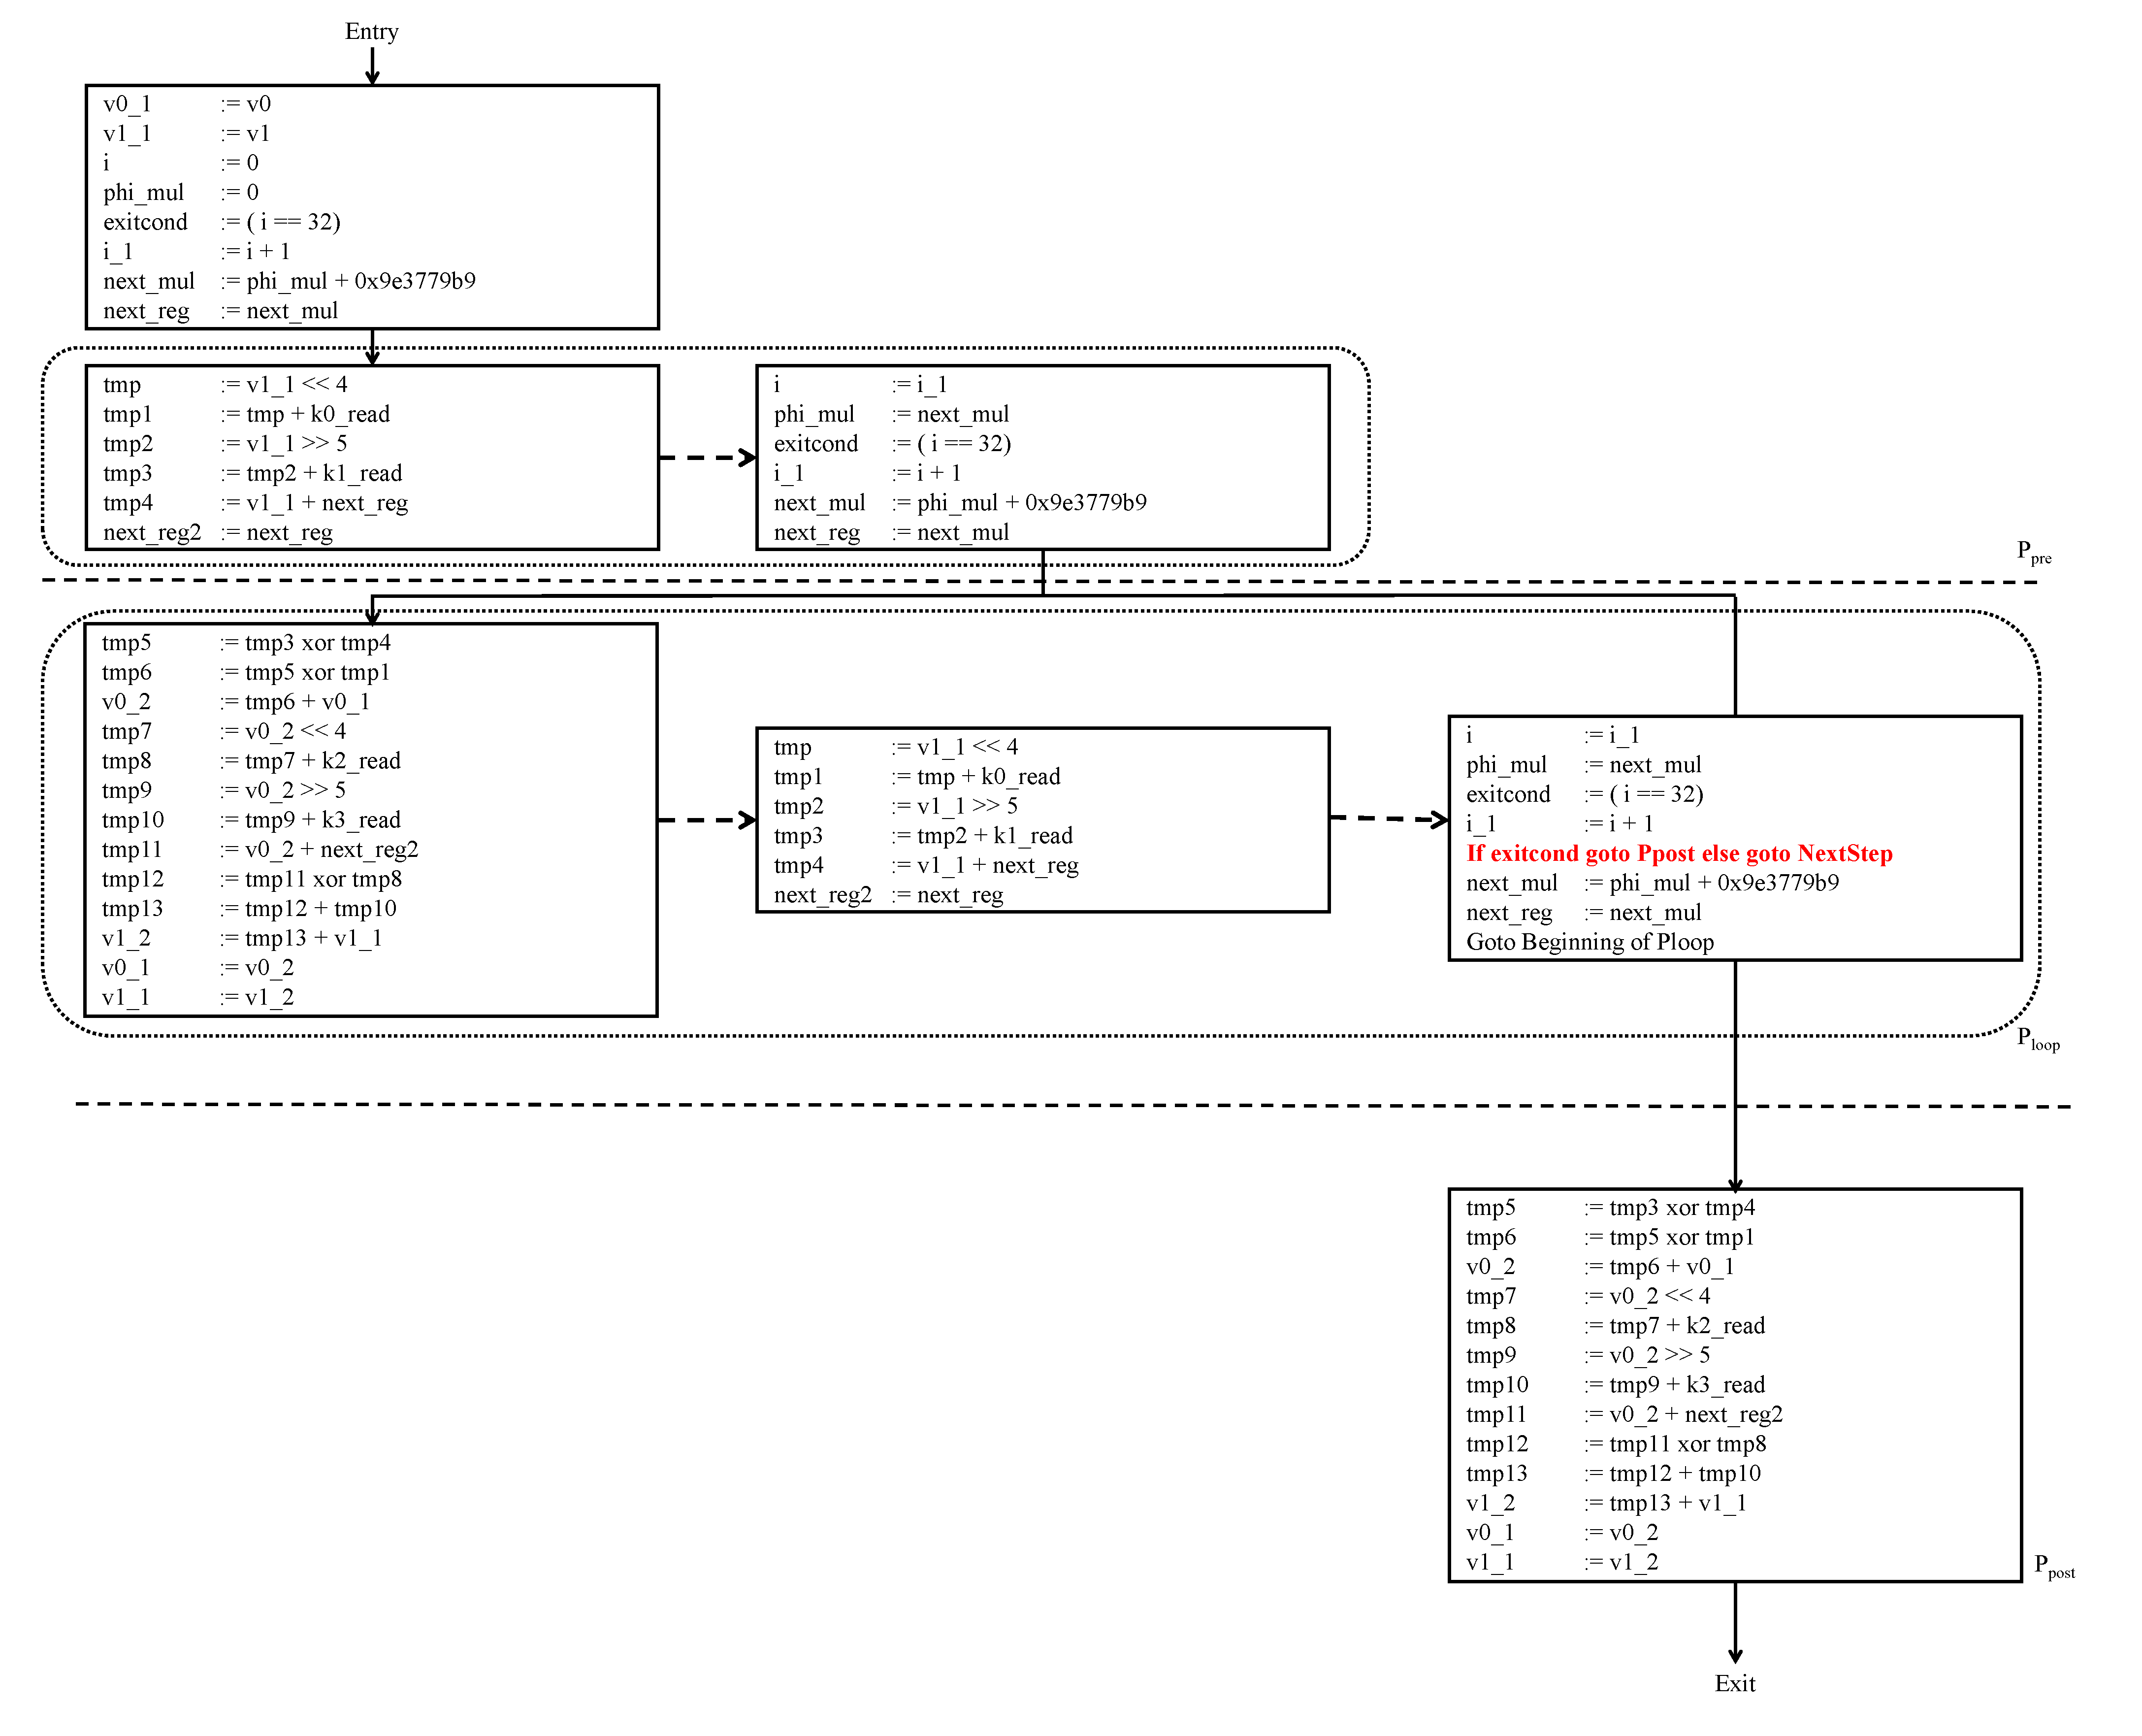
\includegraphics[height=5.5in]{fig-proposal/tea-after-adding-branches}
\end{center}
\caption{TEA: Pipelined CCDFG after adding branches back}
\label{fig:tea-after-adding-branches}
\end{sidewaysfigure}
\clearpage

As is evident from this example, we have a methodical way of dealing with data hazards and ensuring that we can get a smooth pipeline structure. 
We have shown that our approach works by testing it on industrial strength designs. The systematic approach to creating a pipelined structure has enabled 
us to succintly decompose our algorithm into certified primitives and thus certify the overall algorithm.






    \ifoddchapterpage
    \newoddpage
    \fi
    
            %%-------------------------------------------------------------------------
    \chapter{Conslusion and Future Work}
\label{sec:research-plan}

\section{Summary}
Our dissertation is on developing a framework of certified pipelining primitives for building certified pipelining algorithms. We build a loop pipelining algorithm using this framework and certify it using ACL2 theorem prover. We have formalized the syntax and semantics of our intermediate representation (CCDFG) in ACL2. We have successfully identified and formalized a framework of succinct and provable primitives essential for loop pipelining algorithms. These primitives include $\phi$-elimination, shadow-register, interchange, branch and superstep-construction primitive. We have formalize a key invariant, unlike used before for any microprocessor pipeline verification, required for the correspondence between the sequential loop with the backedge and the pipelined loop with the backedge. We have proved that the corresponding relation is true for our algorithm and we have proved the implication chain from this relation to the correctness statement for our algorithm. Using these certified primitives as building blocks and our key invariant, we have formalized and certified a loop pipelining algorithm.
We have proved that each component of our algorithm described in Chapter~\ref{sec:pipelining-algorithm} maintains the invariant that the execution of CCDFGs before and after that component is same. Even though each component essentially decomposes into proving that our primitive is correct, we still have to prove that every application of our primitives maintains certain assumptions and does not disrupt the certification flow. Also, we have proved by induction that applying a primitive in the context of a CCDFG is correct.

%Initially, we proposed a proof sketch certifying that an unrolled sequential loop is equivalent to its unrolled pipelined counterpart. We had planned to extend the unrolled loop to include loops with backedges. However, we realized that there is no direct link between the backedges of the two CCDFGs. While the backedge in the sequential CCDFG involves scheduling steps of a particular iteration in order, the backedge of the pipelined CCDFG includes scheduling steps across different iterations. This led us to identify and formalize our key invariant required for the correspondence between the sequential loop with the backedge and the pipelined loop with the backedge. As of this writing, we have proved that the corresponding relation is true for our algorithm and we have proved the implication chain from this relation to the correctness statement for our algorithm.

Our current ACL2 script has $296$ definitions and $1012$ lemmas, including many lemmas about structural properties of CCDFGs (but not counting those from the false starts). 

Since, we have a certified loop pipelining algorithm, we can confidently say that there are no data hazards and executing a sequential loop is same as executing a pipelined loop created using our algorithm. We have tested the pipeline reference model created using our algorithm on a variety of designs across different application domains. This shows that our algorithm is practical and can be used for industrial strength designs with tens of thousands of RTL. 

With this dissertation, we have made the following major contributions:
\begin{enumerate}[--]
\item {\em Developed a framework of succinct certified primitives essential to build pipelining algorithms} : Our primitives are essential for developing certified loop pipelining algorithm in behavioral synthesis. This framework can also be extended to certify other pipelining algorithms such as function pipelines.
\item {\em Designed and certified a reference loop pipelining algorithm} : We utilize our framework of certified primitives as backbone to build our certified loop pipelining algorithm. Since a primitive can only be applied under certain conditions, when certifying the algorithm, we prove that every application of our primitive is under correct conditions and certain assumptions are maintained after the application of a primitive. We also formalize and certify a key invariant for the correspondence between the sequential and pipelined CCDFGs and propose an algorithm for handling branch conditions in pipelines.
\item {\em Evaluated our algorithm on industrial-strength designs} : We test our algorithm on a variety of designs across different application domains. If our algorithm can generate a pipeline reference model for a design, we can compare it to the pipelined RTL generated by behavioral synthesis tools using SEC. If the SEC passes, we certify the application of loop pipelining transformation is correct. We show that our algorithm can discharge industrial-strength designs.
\end{enumerate} 

\section{Next Steps}
Our dissertation shows that it is possible to develop and certify an industrial-strength loop pipelining algorithm if we can decompose it into succint certifiable primitives. We have already identified and certified these primitives. Our algorithm has components which can identify data hazards based on the given pipeline interval. Then we use our certified primitives to remove those data hazards and create a pipelined implementation.

Function pipelining algorithms also have the same type of data hazards as we have mentioned in loop pipelining algorithms. However, while loop pipelines have a fixed pipeline interval which is known at compile time, function pipelines have a variable pipeline interval for every iteration. So, instead of identifying data hazards at once for every iteration, we would have to call those functions for each iteration. After we have identified the data hazards, we can use our certified primitives to remove those data hazards. We believe that if we can modify the algorithm to identify data hazards, then we can conveniently reuse our certified primitives to certify behaviorally synthesized function pipelines as well.     
    \ifoddchapterpage
    \newoddpage
    \fi

    \bibliographystyle{plain}
    \bibliography{bib}


\end{document}

%%%\begin{document}
%%%
%%%\renewcommand{\textfraction}{0.10}
%%%\renewcommand{\topfraction}{0.90}
%%%\renewcommand{\bottomfraction}{0.70}
%%%\renewcommand{\floatpagefraction}{0.90}
%%%
%%%\input{abstract}
%%%
%%%\setcounter{tocdepth}{2}
%%%\tableofcontents
%%%\newpage
%%%
%%%\input{introduction/introduction}
%%%
%%%\input{background/background}
%%%
%%%\input{sevd/sevd}
%%%
%%%\input{coverage/coverage}
%%%
%%%\input{actg/actg}
%%%
%%%\input{adfi/adfi}
%%%
%%%%\input{plan}
%%%
%%%%\bibliographystyle{splncs}
%%%\bibliographystyle{plain}
%%%\bibliography{dissertation}
%%%
%%%\end{document}
